%%%%%%%%%%%%%%%%%%%%%%%%%%%%%%  IEEEsample.tex
%%%%%%%%%%%%%%%%%%%%%%%%%%%%%%%%%%%%%%%%%
%%%%%%%%%%%%%%%%%%%%%%%    More information: see the header of IEEEtran.sty
%%%%%%%%%%%%%%%%%%%%%%%
%%%%%%%%%%%%%%%%%%%%%%%%%%%%%%%%%%%%%%%%%%%%%%%%%%%%%%%%%%%%%%%%%%%%%%%%%%%%%%%%
%%%%

\documentclass[10pt,twoside,onecolumn]{IEEEtran}
%\documentclass[conference]{IEEEtran}

%%%\IEEEoverridecommandlockouts

\usepackage[ruled,linesnumbered]{algorithm2e}
%%for algorithm2e package, label has to be following caption in the same line!!!
\renewcommand{\algorithmcfname}{ALGORITHM}
\SetAlFnt{\small}
\SetAlCapFnt{\small}
\SetAlCapNameFnt{\small}
\SetAlCapHSkip{0pt}
\IncMargin{-\parindent}

%% \RequirePackage{times}
%% \RequirePackage{algorithmic}
%% \PassOptionsToPackage{boxed}{algorithm}
%% \RequirePackage{algorithm}
%% \RequirePackage{multicol}
%\renewcommand{\algorithmicrequire}{\textbf{Inputs:}}
%\renewcommand{\algorithmicensure}{\textbf{Outputs:}}
%\DeclareMathAlphabet{\mathtsl}{OT1}{ptm}{m}{sl}

%\def\BibTeX{{\rm B\kern-.05em{\sc i\kern-.025em b}\kern-.08em1
%    T\kern-.1667em\lower.7ex\hbox{E}\kern-.125emX}}

%\newtheorem{theorem}{Theorem}
%\newtheorem{lemma}{Lemma}
%\newtheorem{example}{Example}
%\newtheorem{corollary}{Corollary}

\RequirePackage{amssymb, mathptm}
% \usepackage{amsbsy}
% \usepackage{amsthm}
% \usepackage{graphicx}
% \usepackage{helvet}
% \usepackage{enumerate}
% \usepackage{amsmath}
% \usepackage{amsfonts}
% \usepackage{graphicx}
% \usepackage{multirow}
% \usepackage{subfig}
% \usepackage{comment}
% \usepackage{cases}
% \usepackage{leqno}
% \usepackage{subfigure}
\usepackage{amsbsy}
\usepackage{amsthm}
\usepackage{graphicx}
\usepackage{helvet}
\usepackage{enumerate}
\usepackage{amsmath}
\usepackage{amsfonts}
\usepackage{graphicx}
\usepackage{multirow}
\usepackage{subfig}
\usepackage{comment}
\usepackage{cases}
\usepackage{xcolor}
\usepackage{epstopdf}
\usepackage[normalem]{ulem}

%%indent in algorithm


%\setcounter{page}{1}


% New command for the table notes.
\def\tabnote#1{{\small{#1}}}

% New command for the line spacing.
\newcommand{\ls}[1]
    {\dimen0=\fontdimen6\the\font
     \lineskip=#1\dimen0
     \advance\lineskip.5\fontdimen5\the\font
     \advance\lineskip-\dimen0
     \lineskiplimit=.9\lineskip
     \baselineskip=\lineskip
     \advance\baselineskip\dimen0
     \normallineskip\lineskip
     \normallineskiplimit\lineskiplimit
     \normalbaselineskip\baselineskip
     \ignorespaces
    }
%\renewcommand{\algorithmicrequire}{\textbf{Input:}}
%\renewcommand{\algorithmicensure}{\textbf{Output:}}

\newcommand{\beq}{\begin{equation}}
\newcommand{\eeq}{\end{equation}}
\newcommand{\beqarr}{\begin{eqnarray}}
\newcommand{\eeqarr}{\end{eqnarray}}
%\newcommand{\ov}{\overline}
\newcommand{\ov}{\bar}
\newcommand{\xor}{\bigoplus}
\newcommand{\Fm}{{\mathbb{F}}}
\newcommand{\myfontsize}{\fontsize{7}{9}\selectfont}


%the following is for space before and after align or other equation environment.

%%
\newtheorem{Algorithm}{Algorithm}[section]
\newtheorem{Definition}{Definition}[section]
\newtheorem{Example}{Example}[section]
\newtheorem{Proposition}{Proposition}[section]
\newtheorem{Lemma}{Lemma}[section]
\newtheorem{Theorem}{Theorem}[section]
\newtheorem{Corollary}{Corollary}[section]
\newtheorem{Conjecture}{Conjecture}[section]
\newtheorem{Problem}{Problem}[section]
\newtheorem{Notation}{Notation}[section]
\newtheorem{Setup}{Problem Setup}[section]

%%%

%%set spacing between table columns
\setlength{\tabcolsep}{3pt}

\begin{document}

%\thispagestyle{empty}
%\pagestyle{empty}

%\ls{1.5}
% 

\ls{1.1}

\title{\large{\textsc{Sequential Circuit Verification at Word Level Using Algebraic Geometry}}}
\author{Xiaojun Sun\\
A Ph.D Dissertation Proposal\\
Electrical \& Computer Engineering, University of Utah\\
Spring Semester 2015
}
\maketitle

%\markboth{MS Proposal by Tim Pruss}{}
\newcommand{\Fq}{{\mathbb{F}}_{q}}
\newcommand{\Fkk}{{\mathbb{F}}_{2^k}}
\newcommand{\Ftwo}{{\mathbb{F}}_{2}}
\newcommand{\Fkkx}[1][x]{\ensuremath{\mathbb{F}}_{2^k}[#1]\xspace}
\newcommand{\Grobner}{Gr\"{o}bner\xspace}
\newcommand{\B}{{\mathbb{B}}}
\newcommand{\Z}{{\mathbb{Z}}}
\newcommand{\F}{{\mathcal{F}}}
\newcommand{\G}{{\mathcal{G}}}
%%%

\newcommand{\debug}[1]{\textcolor{gray}{[ #1 ]}}


%%%%%%%%%%%%%%%%%%%% Include your files here %%%%%%%%%%%%%%%%%%%%%

% \section{Algebraic Geometry Concepts and Boolean Satisfiability}
\subsection{History}
Boolean satisfiability (SAT) problem is one of most basic problems in computer science.
It is the essential problem for a large number of circuit testing and verification problems.
Fig.\ref{fig:SAT} shows a simple example of SAT problem on circuits verification:
we need to verify whether subcircuit $A$ and subcircuit $B$ has the same function, so
we build a miter circuit for their outputs $X$ and $Y$, and the equivalence checking 
problem is turned into a SAT problem as follows:
\begin{align*}
&Is\ subcircuit\ A\ functionally\ equivalent\ to\ subcircuit\ B?\\
&\Longleftrightarrow
Is\ it\ true\ that\ no\ Boolean\ vector\ assignment\ to\ primary\ inputs\ a,b,c\ such\ that\ Z=1?
\end{align*}

\begin{figure}[hbt]
\centering{
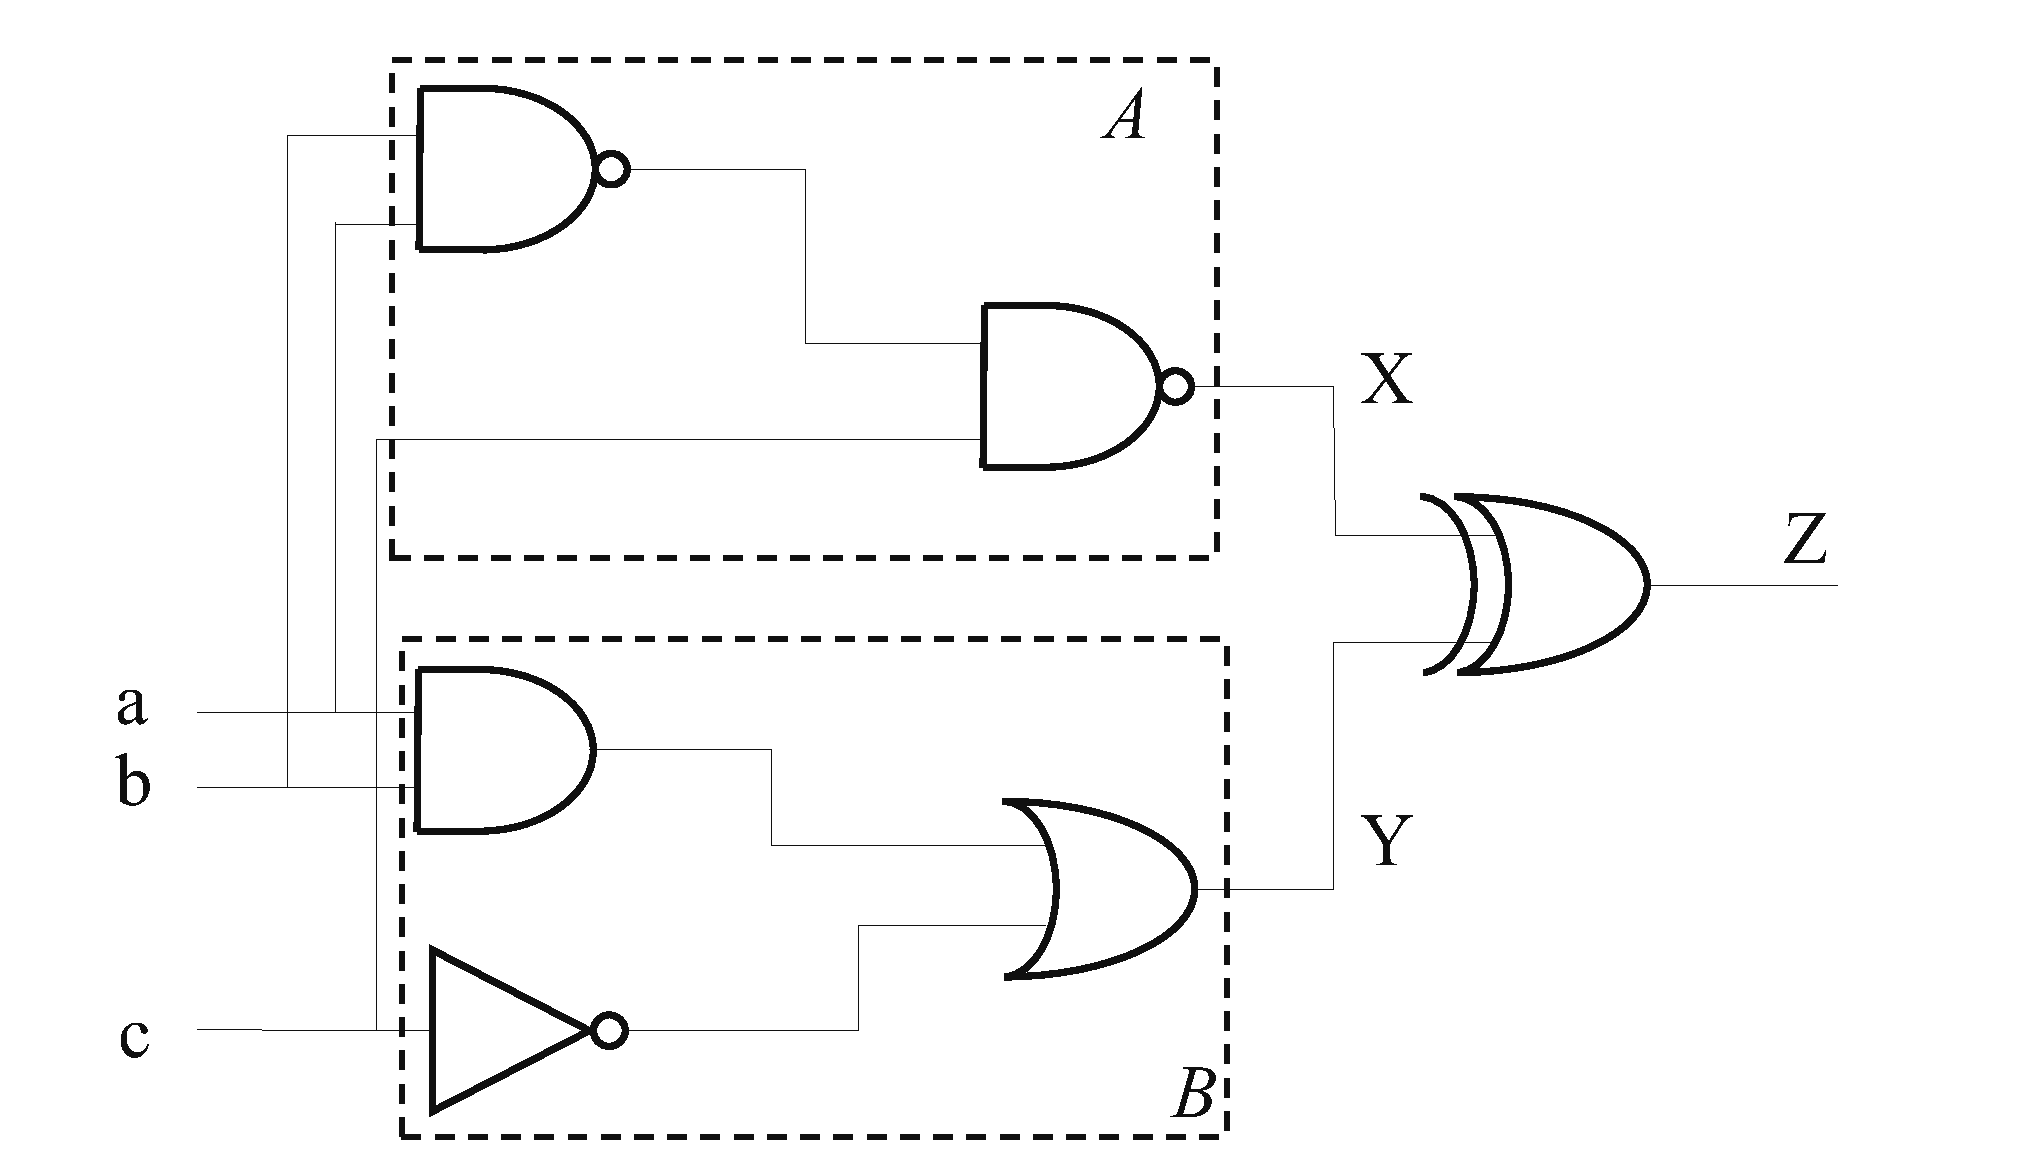
\includegraphics[scale=0.3]{./fig_SAT.eps}
\caption{An example of Boolean satisfiability problem on circuits}
\label{fig:SAT}}
\end{figure}


In most cases, SAT problems are modeled as CNF formulas, and solved by procedures based on 
Davis-Putnam and Davis-Logemann-Loveland (DPLL) algorithm. The main idea of DPLL algorithm
is recursive branching and backtrack searching. To improve the efficiency of DPLL-based
SAT solver, efforts are made on minimizing number of branches, accelerating unit propagation
and modifying backtrack algorithm. Recently state-of-art SAT solvers developed conflict-driven
clause learning (CDCL) technique to prune the search space, which is effective to reduce
result search time.

On the other hand, people are seeking an alternative solution for SAT problem using a totally
different method from ``old-fashioned" DPLL algorithm. One promising option is polynomial calculus (PC),
mapping Boolean variables and connectors in CNF formulas to variables and operators in 
Galois fields. In this way clauses are transformed to monomials/polynomials, thus theorems and concepts in computer
algebra such as Hilbert's Nullstellensatz and Gr\"obner basis can be employed to assist finding
valid assignments or proof of unsatisfiability. Basic concepts about PC will be formally introduced with definitions
from computer algebra.

The inspiration that use PC to solve SAT problems first comes from \cite{ceiSTOC96}.
Using PC and its variations, researchers develop many SAT solvers \cite{STABLE} \cite{BLUEVERI} \cite{PolyBoRi} 
Besides, people borrow concepts from PC, combine them with traditional DPLL and clause learning techniques
to build hybrid SAT solvers. \cite{condratTACAS07} \cite{Zengler2010}
\subsection{Define SAT problem in computer algebra}
\label{sec:mapping}
In this part, we formally define SAT problems in language of computer algebra by mapping CNF formulas to polynomials.
First, Boolean variables are mapped to field/ring elements, so it is necessary to introduce the concept of field
and ring.
\begin{Definition}
A {\bf ring} is a set with binary operators ``$+$" and ``$\cdot$" satisfying:\\
(1.a) ``$+$" is associative and commutative;\\
(1.b) There exist element $0$ as additive identity, and every element has additive inverse;\\
(2.a) ``$\cdot$" is associative;\\
(2.b) There exist element $1$ as multiplicative identity;\\
(3) Multiplication distributes over addition.
\par
A {\bf field} is a ring satisfying:\\
(1) every nonzero element has multiplicative inverse;\\
(2) ``$\cdot$" is commutative.
\par
A field containing finite number of elements is called {\bf finite field}, or {\bf Galois field}.
\end{Definition}
\begin{Example}
Consider the set of all integers $\mathbb Z$ and usual definition of addition ``$+$" and multiplication ``$\cdot$".
Then $\mathbb Z$ is a ring. But it is not a field because some integers do not have multiplicative inverse: 
$\frac{1}{2} \notin \mathbb Z$. The set of all rational numbers $\mathbb Q$ is a field, but not a Galois
field since it has infinite number of elements. An example of Galois field is the set of integers modulo a prime
($\mathbb Z/n\mathbb Z,\ n$ is prime), e.g. Galois filed $\mathbb F_5$ can be interpreted as set of 5 integers
$\{0,1,2,3,4\}$, and addition/multiplication defined as $a+b\pmod 5,\ a\cdot b\pmod 5$.
\end{Example}
In some cases a field $\mathbb F$ can be extended to a ring. If we take indeterminates $x_1,x_2,\dots,x_n$ 
(usually not from field $\mathbb F$), an arbitrary combination of their finite product 
$x_1^{d_1}\cdot x_2^{d_2}\cdots x_n^{d_n}$ is a {\bf monomial}. A {\bf polynomial} $f = c_1 X_1 +
c_2 X_2 + \dots + c_t X_t$ is a finite sum of terms, where $c_1,
\dots, c_t$ are coefficients and $X_1, \dots, X_t$ are monomials.
These polynomials can form a ring, if coefficients come from elements of $\mathbb F$, we call this ring as
a {\bf multivariate polynomial ring} $\mathbb F[x_1,\dots,x_n]$.
\begin{Example}
\label{ex:polyring}
Ring $\mathbb Z[a,b,c]$ contains elements such as $4a^3b+7ab^2c+2c^2$, and ring $\mathbb F_2[a,b,c]$
contains elements such as $a+bc+1$, which can be mapped to a Boolean CNF formula!
\end{Example}
$k$-variable CNF clauses for SAT are defined over Boolean ring $\mathbb B^k$. We can define a unique 
mapping $\mathbb B^k \to \mathbb F_2[x_1,\dots,x_k]$ to transform a CNF formula to polynomial,
including:
\begin{align*}
T &\to 1\\
F &\to 0\\
\land &\to \cdot\\
\oplus &\to +\\
\text{Boolean variables} &\to \text{ field } \mathbb F_2 \text{ elements }
\end{align*}
Namely we can represent Boolean connectors $\neg,\ \bar{\oplus},\ \lor$ as:
\begin{align*}
&\neg a \to 1+a\\
&a \bar{\oplus} b \to 1+a+b\\
&a \lor b \to a+b+a\cdot b
\end{align*}
Using these mappings it is easy to write CNF clauses to polynomials accordingly.
The most straightforward way to solve SAT problem in form of polynomials is to create
equations that each polynomial equals to 1, then solve the system of equations.
Solutions to the system is defined as affine varieties:
\begin{Definition}
Given a set of polynomials $f_1,\dots,f_k$ over ring $\mathbb F_q[x_1,\dots,x_n]$, their 
{\bf affine variety} 
$$V(f_1,\dots,f_k) = \{(a_1,\dots,a_n)\in \mathbb F_{q^n} | f_1(a_1,\dots,a_n) = \cdots = f_k(a_1,\dots,a_n) = 0\}$$
\end{Definition}
Different sets of polynomials may have same variety. There is a method to find out the set of
all polynomials with the same variety, which is 
\begin{Definition}
{\bf Ideal of Polynomials:} Let $f_1,f_2,\dots,f_s\in \mathbb F[x_1,\dots,x_n]$.
Define an ideal
$$J = \langle f_1,f_2,\dots,f_s\rangle = \{f_1\cdot h_1 + f_2\cdot h_2 +\cdots + f_s\cdot h_s : h_1,\dots,h_s\in \mathbb F[x_1,\dots,x_n]\}$$
We call $J = \langle f_1,f_2,\dots,f_s\rangle$ an ideal generated by $f_1,\dots,f_s$ and these polynomials 
the {\bf generators} of ideal $J$.
\end{Definition}
On the other hand, if given another polynomial $f$, we need to judge whether it belongs to $J$.
\begin{Definition}
{\bf Ideal membership:} Let $f_1,f_2,\dots,f_s\in \mathbb F[x_1,\dots,x_n]$, and $J = \langle f_1,f_2,\dots,f_s\rangle$
be an ideal over ring $\mathbb F[x_1,\dots,x_n]$. If 
$$f = f_1h_1 + f_2h_2 + \cdots + f_sh_s$$
then $f\in J$.
\end{Definition}
We can easily deduce varieties of $J$ will also vanish on polynomial $f$, i.e. if 
$f_1({\bf a}) = f_2({\bf a}) = \cdots = f_s({\bf a}) = 0$, then $f({\bf a}) = 0$.
\subsection{The structure of affine variety and algebraic Geometry}
The structure of affine variety is straightforward when analyzing from geometry view. Consider
ring $\mathbb F[x_1,\dots,x_n]$, it can be interpreted as a $n$-dimension space, and
coordinates are elements from field $\mathbb F$. Affine varieties on this ring are
sets of dots in the space.
\begin{Example}
(Fig.\ref{fig:variety}) Consider ring $\mathbb R[x,y]$, it is a plane with Cartesian coordinates $(x,y)$. Variety of a single-generator 
ideal $J = \langle x^2+y^2-1\rangle$ is all points on center $(0,0)$ radius $1$ circle.
$$V_{\mathbb R}(\langle x^2+y^2-1\rangle) = \{(x,y)|x^2+y^2=1,\ x,y\in \mathbb R\}$$
Meanwhile variety depends on the ring where ideal locates, e.g. for ring $\mathbb R[x]$
$$V_{\mathbb R}(\langle x^2+1\rangle) = \emptyset$$
while for ring allowing complex numbers $\mathbb C[x]$
$$V_{\mathbb C}(\langle x^2+1\rangle) = \{\pm i\}$$
\end{Example}

\begin{figure}[hbt]
\centering{
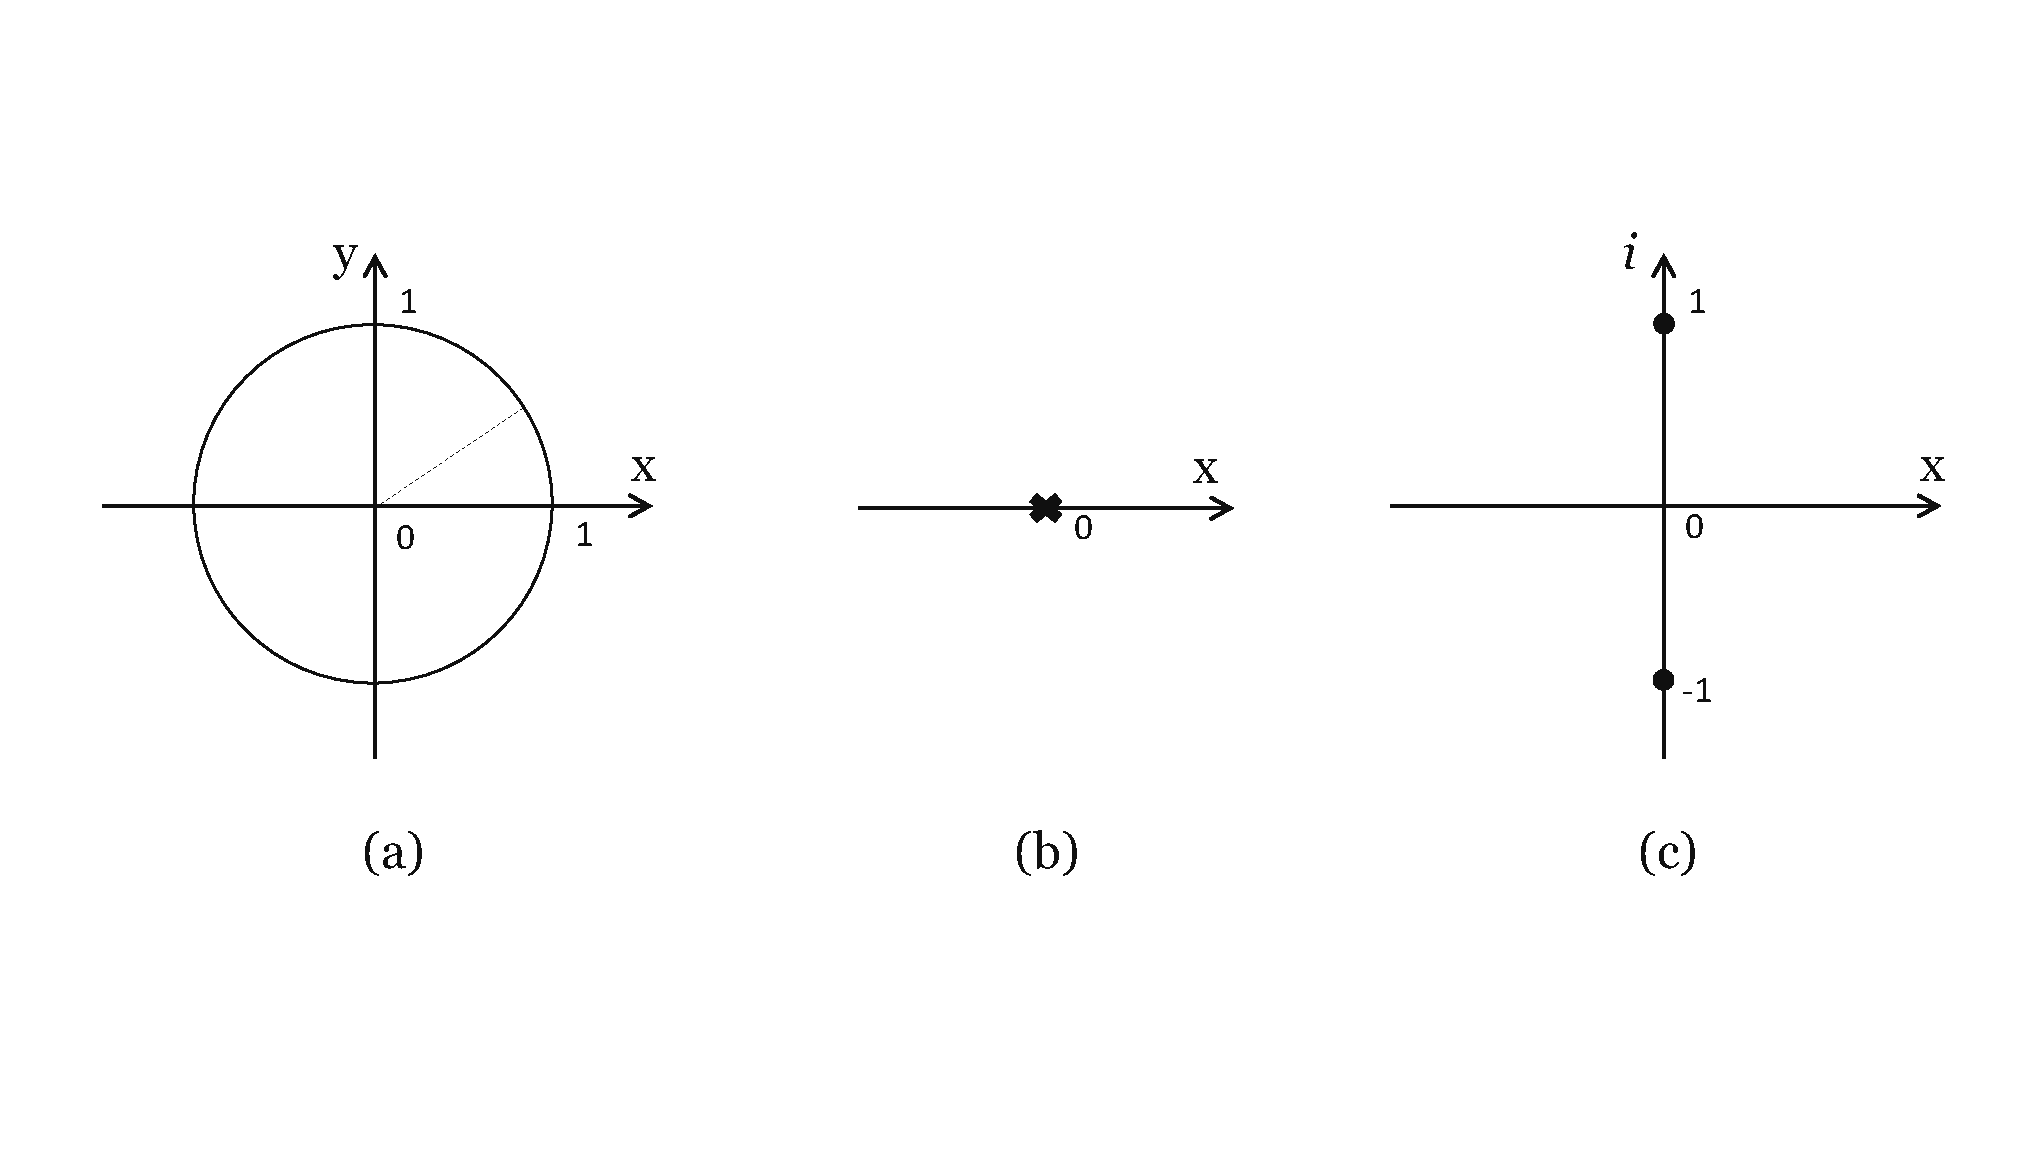
\includegraphics[scale=0.5]{./fig_variety.eps}
\caption{Examples of affine varieties in affine space}
\label{fig:variety}}
\end{figure}
Applying set manipulations such as {\bf union}, {\bf intersection} and {\bf complement} to varieties 
and ideals is an important topic to explore. First, we introduce following concepts from algebraic geometry:
\begin{Definition}
\label{def:sum}
({\bf Sum of Ideals}) If $I$ and $J$ are ideals in $\mathbb F[x_1, \dots, x_n]$, then the 
{\bf sum} of $I$ and $J$, denoted by $I + J$, is the set
  \begin{equation}
  I + J = \{f + g\ |\ f \in I \ and\  g \in J\}.
  \end{equation}
Furthermore, if $I = \langle f_1, \dots, f_r\rangle$ and 
$J = \langle g_1, \dots, g_s\rangle$, then 
$I + J = \langle f_1, \dots, f_r, g_1, \dots, g_s\rangle$.
\end{Definition}
\begin{Definition}
\label{def:prod}
({\bf Product of Ideals}) If $I$ and $J$ are ideals in $\mathbb F[x_1, \dots, x_n]$, then the
{\bf product} of $I$ and $J$, denoted by $I \cdot J$, is defined to be the ideal generated 
by all polynomials $f \cdot g$ where $f \in I$ and $g \in J$. Furthermore, let
$I = \langle f_1, \dots, f_r\rangle$ and $J = \langle g_1, \dots, g_s\rangle$, then
  \begin{equation}
  I \cdot J = \langle f_ig_j\ |\ 1 \leq i \leq r, 1 \leq j \leq s\rangle .
  \end{equation}
\end{Definition}
\begin{Definition}
({\bf Quotient of Ideals}) If $I$ and $J$ are ideals in $\mathbb F[x_1, \dots, x_n]$, then $I:J$
is the set
  \begin{equation}
  \{f \in \mathbb F[x_1, \dots, x_n]\ |\ f\cdot g \in I, \forall g \in J\}
  \end{equation}
and is called the {\bf ideal quotient} of $I$ by $J$.
\end{Definition}
These concepts can lead the way to solution by adopting following theorems:
\begin{Theorem}
\label{thm:unionintersect}
If $I$ and $J$ are ideals in $\mathbb F[x_1, \dots, x_n]$, then ${\bf V}(I + J) = {\bf V}(I)
\bigcap {\bf V}(J)$ and ${\bf V}(I \cdot J) = {\bf V}(I) \bigcup {\bf V}(J)$.
\end{Theorem}
However, complement of variety cannot be easily dealt by simple arithmetic on polynomial generators.
For non-trivial cases we can only prove that 
\begin{Theorem}
Let $I, J$ be ideals in $\mathbb F[x_1,\dots,x_n]$, then 
$${\bf V}(I:J) \supset {\bf V}({\bf I}({\bf V}(I) - {\bf V}(J)))$$
\end{Theorem}

Fortunately for most hardware verification cases, the form of polynomial generators are restricted.
A proposition has been proved by \cite{jinpeng} that after adding {\bf vanishing polynomials ideal}
the new composed ideal is {\bf radical}, which implies following corollary can be employed:
\begin{Corollary}
\label{thm:quotient}
Let $I, J$ be radical ideals in $\mathbb F[x_1,\dots,x_n]$, then 
$${\bf V}(I:J) = {\bf V}(I) - {\bf V}(J)$$.
\end{Corollary}
The variety of vanishing polynomial ideal contains all possible evaluations of variables, so it
is the {\bf universal set}. Subsequently, the {\bf absolute complement} can be written as
$$\overline{{\bf V}(J)} = {\bf V}(J_0:J)$$

\subsection{Gr\"obner basis and UNSAT}
Different generators may generate the same ideal, which means we can equivalently transform one set of generators
to another for computational or theoretical convenience.
Some generators are "optimal" representation of the ideal, such as {\bf Gr\"obner basis}.

Gr\"obner basis contains generators whose leading monomials can divide the leading monomials of all polynomials 
in the ideal:
\begin{Definition}
A set of polynomials $G = \{g_1,\dots,g_t\}$ is the Gr\"obner basis (GB) of ideal $J$ if and only if
$$\forall f\in J, \exists g_i,\ s.t.\ LM(g_i)\mid LM(f)$$
\end{Definition}
The advantage of representing an ideal with GB is that it can serve as decision procedure for ideal membership
test when dividing polynomial by GB, i.e.
$$G = GB(J) \Longleftrightarrow \forall f\in J, f\xrightarrow{g_1,g_2,\dots,g_t}_{+} 0$$
Gr\"obner basis can be reduced by eliminating redundant elements. A reduced GB is a canonical representation of 
the ideal under some monomial orderings.

When an ideal has empty variety, its reduce GB has a very special form:
\begin{Theorem}
{\bf Weak Nullstellensatz:} Given ideal $J\subset \mathbb F[x_1,\dots,x_n]$, its variety over algebraic closure
of field $\mathbb F$ is null if and only if its reduced Gr\"obner basis contains only one generator ``1".
$${\bf V}_{\overline{\mathbb F}}(J) = \emptyset \Longleftrightarrow reducedGB(J) = \{1\}$$
\end{Theorem}

It is well learned that using Buchberger's algorithm and its variations to compute a GB has a very high
time complexity and is usually not practicable. One reason is that the size of GB may explode even the term
ordering is carefully chosen. However if the reduced GB is 1, which means every term in original polynomials
will be canceled, the degree of newly added GB will be limited. Thus the size of GB is less possible to grow 
too fast. Instead of applying polynomial calculus to SAT solving, it may be more efficient to try UNSAT
problems.

One of most important research topics about UNSAT problem is to find out UNSAT core efficiently.
\begin{Definition}
Assume a set of polynomials $F$ and its subset $F_s\subset F$. If ${\bf V}(\langle F\rangle) = {\bf V}
(\langle F_s\rangle) = \emptyset$, we call $F_s$ an {\bf UNSAT core} of $F$. Additionally, if
$F_s$ has no UNSAT core of itself, we call it a {\bf minimal} UNSAT core.
\end{Definition}

We propose a conjecture based on observation of Buchberger's algorithm's execution.
\begin{Conjecture}
By tracking s-polynomial computations and multivariate divisions that lead to remainder (newly added GB)
1, we can obtain an UNSAT core; we can figure out a minimal UNSAT core at high probability with limited
iterations of execution of Buchberger's algorithm.
\end{Conjecture}
\begin{Example}
A SAT problem is described with 8 CNF clauses:
\begin{align*}
&\bar{a}\lor\bar{b}\\
&a\lor\bar{b}\\
&\bar{a}\lor b\\
&a\lor b\\
&x\lor y\\
&y\lor z\\
&b\lor \neg y\\
&a\lor x\lor \neg z
\end{align*}
Using mappings mentioned in section \ref{sec:mapping}, we can transform them to
polynomials over ring $\mathbb F_2[a,b,x,y,z]$:
\begin{align*}
&f_1:ab\\
&f_2:ab+a\\
&f_3:ab+b\\
&f_4:ab+a+b+1\\
&f_5:xy+y+x+1\\
&f_6:yz+y+z+1\\
&f_7:by+y\\
&f_8:axz+az+xz+z
\end{align*}
We compute its GB using Buchberger's algorithm with lexicographic term ordering $a>b>x>y>z$.
Since this problem is UNSAT, we will stop when ``1" is added to GB.
First we compute $Spoly(f_1,f_2)\xrightarrow{\ }_{+} r_1$, remainder $r_1$ equals to $a$;
Next we compute $Spoly(f_1,f_3)\xrightarrow{\ }_{+} r_2$, remainder $r_2$ equals to $b$;
Then we compute $Spoly(f_1,f_4) = a+b+1$, obviously $a+b+1$ can be reduced (multivariate divided) by
$r_1$ and $r_2$, and they can be backtracked to $f_1,f_2,f_3$. The remainder is ``1", so we
conclude that $f_1,f_2,f_3,f_4$ is an UNSAT core for this problem.
\end{Example}
If we start with other term orderings, we may get a larger UNSAT core. By dynamically adjust
term ordering and re-calculate GB, we can get new UNSAT core with smaller size, until
we find minimal UNSAT core or expire runtime limit. (Need more experiments)
% \section{Combine algebraic geometry with abstraction techniques}
\subsection{History of abstraction on sequential circuits}
Traditional method to analyze a sequential circuit is based on explicit state variable encoding
and full states enumerating from initial state and explicit transition function.
With the size of modern sequential circuits increasing, it is infeasible to apply old methods
any longer. Abstraction is a technique to minimize the state space by combining states with certain 
similarities. Sometimes it can effectively lower down the number of states by orders of magnitude,
without affecting the properties we need to verify.

At first abstraction is done manually by designers. In 2000 E. Clarke \cite{clarke2000counterexample}
proposed an automated abstraction: first,
initial abstraction is set up by dividing variables to different clusters based on transition conditions;
then, an ordinary model checking is operated on this abstraction. If a counterexample is given, 
it is further checked to be concrete or not. For a false abstract state or a spurious path 
, the initial abstraction is refined by further splitting the false abstract state. 
A heuristic algorithm keeps refining the abstraction until a real counterexample is found or 
property verified. This technique is based on binary decision diagrams (BDDs), which means
potential risk of memory explosion; meanwhile it still requires an initial abstraction to start with.
So in 2004 L. Zhang and M. Hsiao \cite{zhang2005design} proposed another abstraction method based on CNF-SAT.
This paper uses simplest latch abstraction -- by removing "irrelevant" latches and change them to primary inputs. 
The key idea is to pick those ``irrelevant" latches (variables in $k$-bounded model checking, $k$-BMC) 
according to SAT/UNSAT analysis from $k$-BMC. It improves the $k$-BMC procedure\cite{biere1999symbolic}: 
LTL properties to check for a $k$-bounded machine can be translated to a big CNF and fed to SAT solver. 
If SAT, a concrete counterexample is found. 
If UNSAT, the original method will just increase bound k. In Zhang's paper, the clauses for UNSAT 
(UNSAT cores) are checked for variables do not appear, they are referring to "irrelevant" latches 
at least for first $k$ iterations. 
Thus an abstracted model is obtained and checked with original property. If the abstracted model checking fails, 
then bound $k$ will increase. This method still has disadvantages: it is counterexample-independent,
which means it cannot utilize information from invariants.

Abstraction usually means over-approximation, i.e. properties are true on abstracted machine
are also valid for original states. Craig's interpolation is a sort of abstraction which could be both
over-approximation and under-approximation. In 2003 K. McMillan used Craig's interpolation to improve 
$k$-BMC \cite{mcmillan2003interpolation}. Initially a $k$-length path to failure state $F$ is picked and transformed to 
CNF formula, then split at first transition into prefix and suffix. Then an interpolation $P$ is computed
between prefix and suffix. $P$ over-approximates 1-step reachable states, and under-approximates states 
that cannot reach $F$ in $k$ steps. If no counterexample exposed, path will be split again at second
transition; in this way a precise abstraction can be found for all reachable states.

$k$-BMC with interpolation is a purely incremental model checking approach, and interpolation procedure relies
on UNSAT core analysis. To overcome these weaknesses, a hybrid model checker named as IC3 is developed 
\cite{bradley2011sat} \cite{bradley2011incremental}. (Not related to abstraction really..)
\subsection{Word-level abstraction: Naive abstraction for arithmetic circuits}
Our approach is an abstraction based on word operand definition of datapaths in arithmetic circuits,
and it can be expanded to generic FSM by bundling a set of bit-level variables to one or several word-level variables.
The abstraction polynomial is obtained through computing GB of an elimination ideal using a special term order.

The authors of \cite{pruss:dac14} showed that for any combinational
logic block, a canonical word-level polynomial representation can be
derived through \Grobner bases computed with elimination
orders. Our approach is based on their result, which we reproduce
here:
\begin{Lemma}
(From \cite{pruss:dac14}) Given a combinational circuit $C$ with $k$-bit
  input $A = (a_0, \dots, a_{k-1})$ and $k$-bit output $R = (r_0, \dots,
  r_{k-1})$. Denote by $x_1, \dots, x_d$ all the bit-level
  variables of   $C$. Let $J = \langle f_1, \dots, f_s \rangle \subset
  \Fkk[x_1, \dots, x_d, R, A]$ denote all the polynomials corresponding to the
  logic gates of the circuit. Let $J_0 = \langle x_1^2 - x_1, \dots,
  x_d^2 - x_d, R^q - R, A^q - A \rangle$ be the vanishing ideal, so
  that $J + J_0 = \langle f_1, \dots, f_s, ~~ x_1^2 - x_1, \dots,
  x_d^2 - x_d, R^q - R, A^q - A \rangle$. Compute \Grobner basis $G =
  GB(J + J_0)$ w.r.t. lex term order with $x_1 > x_2 > \dots > x_d > R
  > A$. Then $G_d = G \cap \Fkk[R, A]$ eliminates the internal
  variables $x_1, \dots, x_d$ of the circuit. $G_d$ also contains the
  word-level polynomial $R = \F(A)$ which canonically represents the
  function of the circuit.  
\end{Lemma}

The authors referred to the elimination (lex) order with
$\{\textit{internal variables} \ x_1 > \dots > x_d\} > \{\textit{word-level
  output} \ R\} > \{\textit{word-level input} \ A\}$ as the {\it abstraction
  term order (ATO)}. 
  
One-step transition can also be implemented on word level using ATO. We represent present state (PS) 
with a univariate polynomial about word-level state variable $f(S)$, its variety intersecting with variety of
circuit ideal $J+J_0$ results to polynomial about word-level next state (NS) $g(T)$. Recall theorem \ref{thm:unionintersect},
$$NS = {\bf V}(\langle g\rangle) = {\bf V}(\langle f\rangle + J+J_0) = GB\ with\ ATO(\langle f\rangle + J+J_0)$$
Note that ideal corresponding to next state is an ideal with single univariate polynomial generator.

Reachability analysis is a useful tool when checking sequential equivalence as well as other invariants.
With word-level state variables, we can do implicit state enumeration to provide a picture of 
reachable states. Following algorithm is breadth-first search style state enumeration \cite{KallaPartialScan}:
\begin{algorithm}[hbt]
\SetAlgoNoLine
 \KwIn{Transition functions $\Delta$, initial state $S^0$}

  $from^0 = reached = S^0$\;
  \Repeat{$new^i == 0$}
  {
  	$i \gets i + 1$\;
	$to^i \gets$Img$(\Delta, from^{i-1})$\;
	$new^i \gets to^i \cap \overline{reached}$\;
  	$reached \gets reached \cup new^i$\;
	$from^i \gets new^i$\;
  }
\Return{$reached$}
\caption {Breadth-first Traversal Algorithm}\label{alg:BFS}
\end{algorithm}
\begin{figure}[hbt]
\centering{
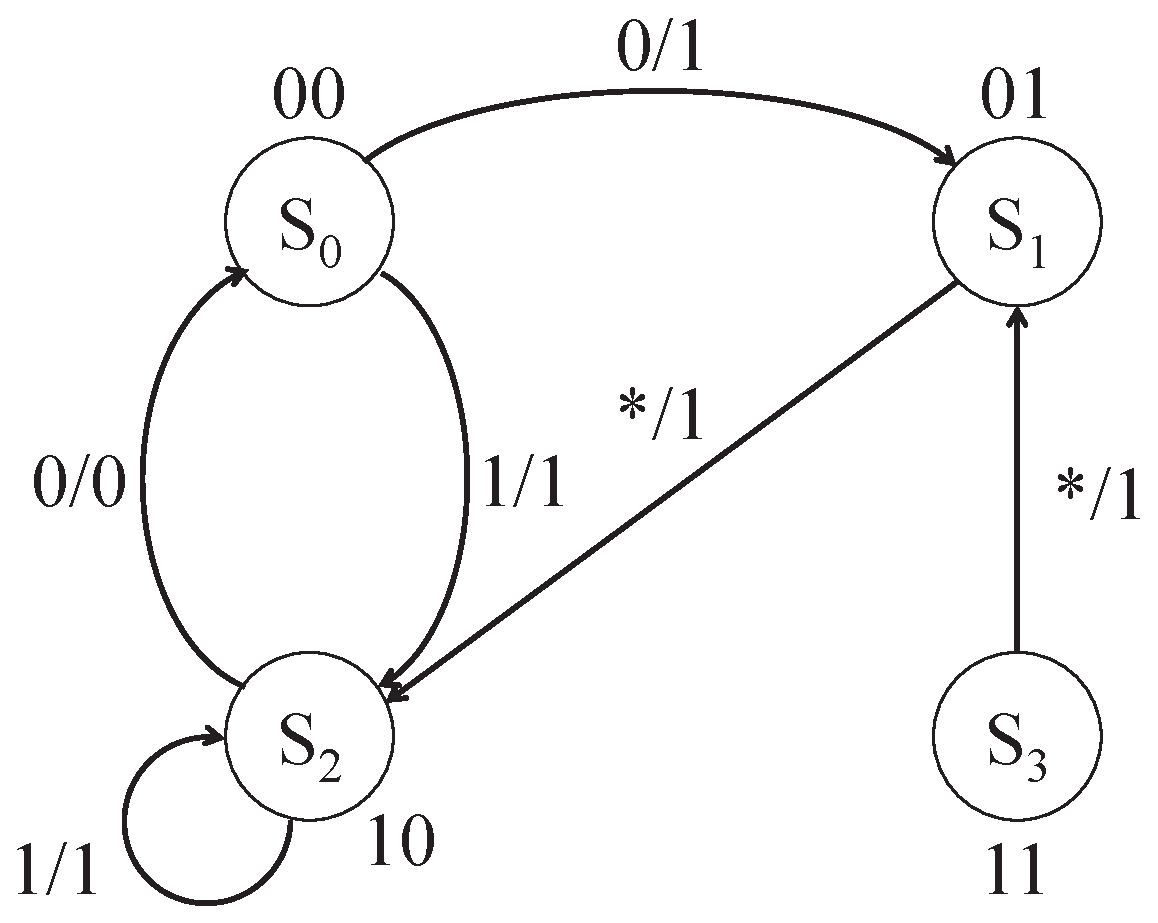
\includegraphics[scale=0.3]{./stg_fig.eps}
\caption{State transition graph of sample FSM}
\label{fig:stg}}
\end{figure}

\begin{figure}[hbt]
\centering{
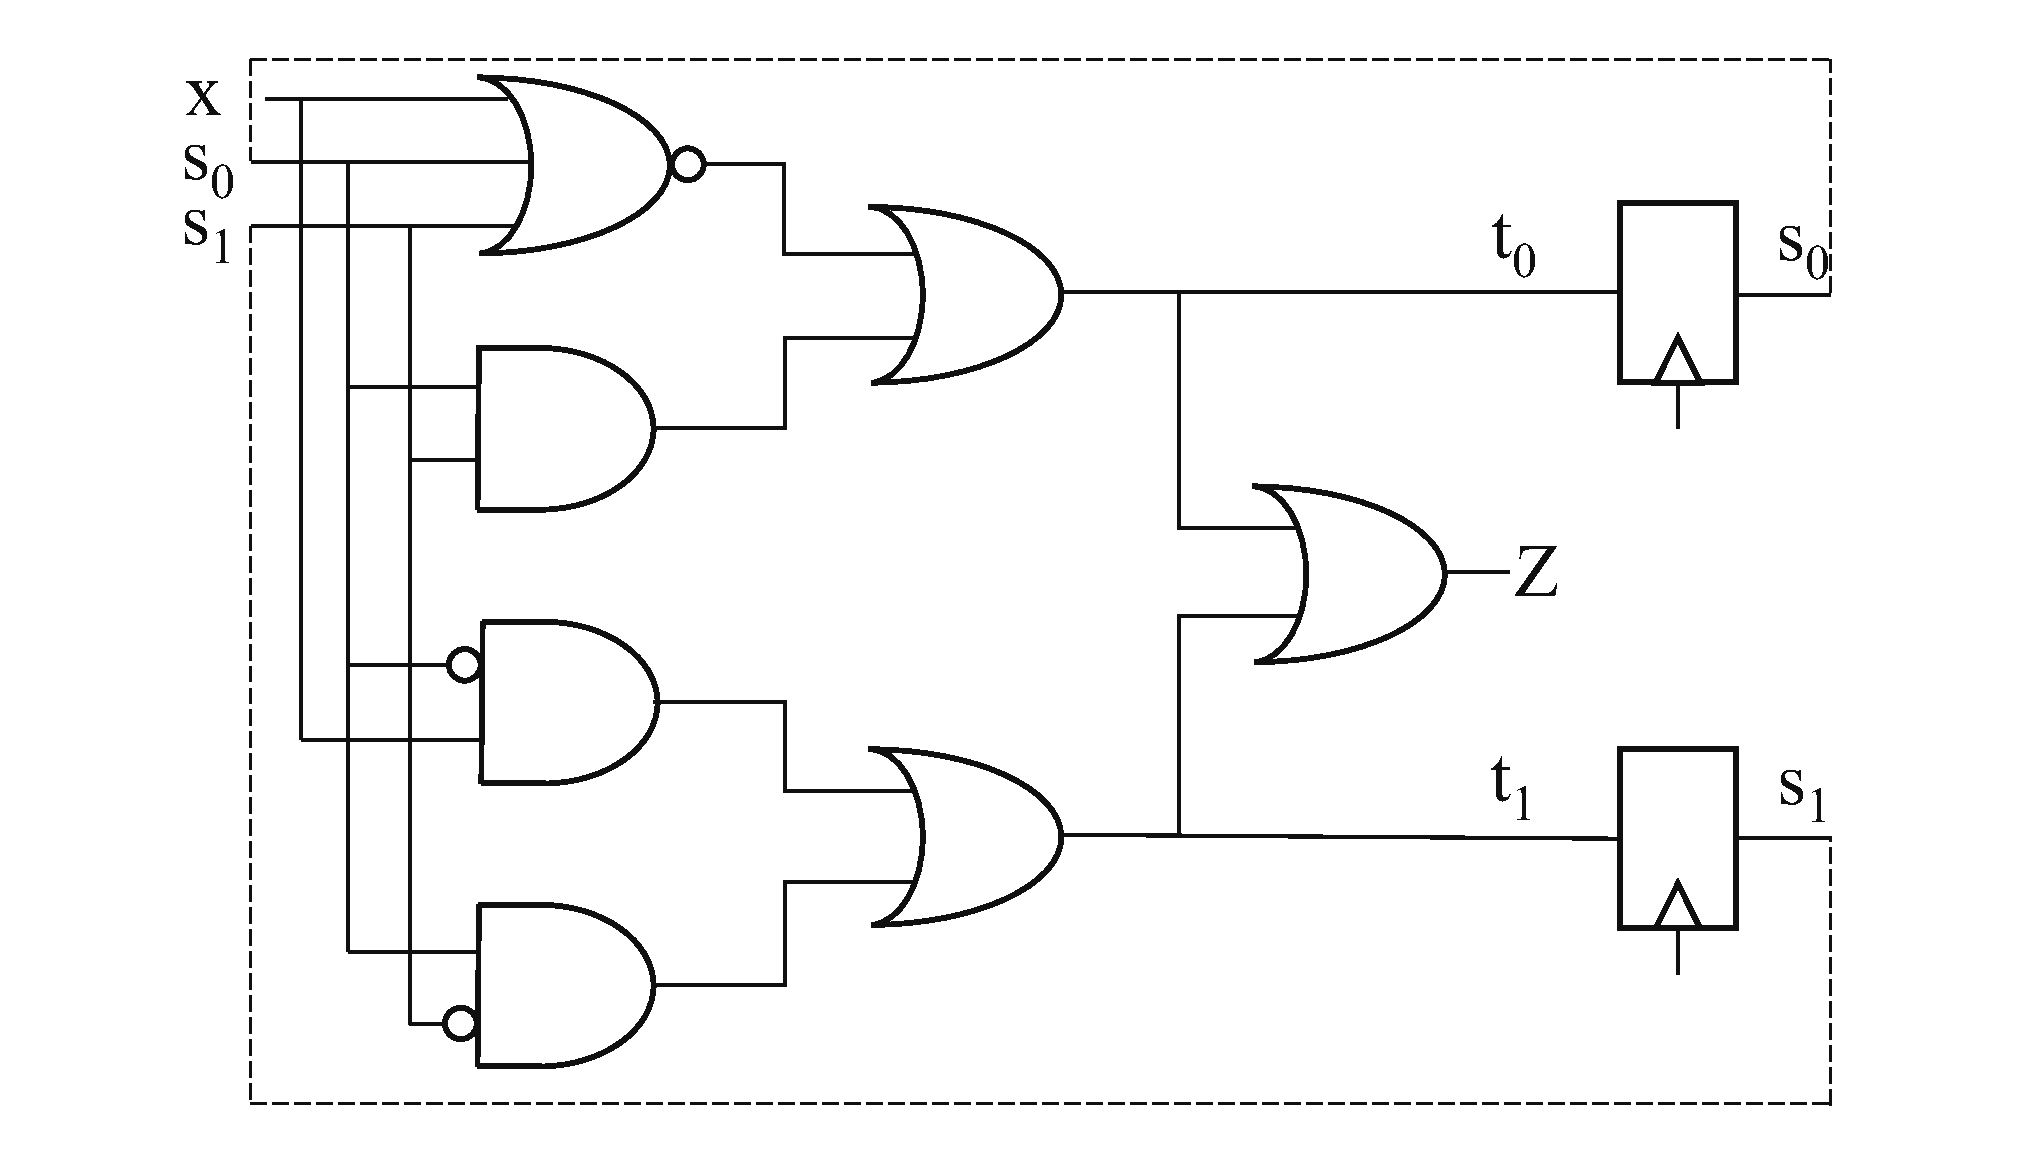
\includegraphics[width=3.5in]{./fsm_fig.eps}
\caption{Gate-level circuit of combinational logic block of sample FSM}
\label{fig:fsm}}
\end{figure}
Here we put a 2-bit Mealy machine as an example showing how to use univariate polynomial ideal
and elimination ideal with ATO to implement this algorithm.
\begin{Example}
\label{ex:2bit}

We are given a mealy Finite State Machine (FSM). Gate-level circuits of combinational logic
is figure \ref{fig:fsm}, $x$ is primary input (one bit),
$\{s_0, s_1\}$ are state inputs, $Z$ is primary output and $\{t_0, t_1\}$ are state outputs.
Word-level state input is $S = s_0 + s_1\cdot\alpha$, output is $T = t_0 + t_1\cdot\alpha$. In Galois field
$\mathbb{F}_{2^2}$, bit-level variables $x, s_0, s_1, Z, t_0, t_1$ can take values from $\{0, 1\}$, while
word-level variables $S, T$ may take values from $\{0, 1, \alpha, 1 + \alpha\}$. State Transition Graph (STG)
showed in figure \ref{fig:stg} uses 2-bit Boolean vector to represent 4 states $\{S_0, S_1, S_2, S_3\}$, which
could be mapped to elements in $\mathbb{F}_{2^2}$.

For example in Line 1 of BFS algorithm, assume initial state is $S_0$ in figure \ref{fig:stg}, then corresponding
polynomial $f = \mathcal{F}(S^0) = S^0 - 0$. Consider an ideal $I$ with only one generator $f$, its variety
$V(I) = \{\gamma\ |\ \gamma \in \mathbb{F}_{2^2}, \gamma = 0\}$, which equals to $\{0\}$, the only
valid value $S^0$ can take.

If an ideal contains multiple polynomial specifications, it is necessary to compute Gr\"obner basis with elimination term
order to get one polynomial only on desired variable. In first iteration of Line 4, $to^i$ has multiple specifications,
some of them are transition functions on bit-level:
\begin{displaymath}
\begin{array}{ll}
f_1:& t_0 - (\overline{x}\ \land\ \overline{s_0}\ \land\ \overline{s_1})\ \lor\ (s_0\ \land\ s_1) \\
f_2:& t_1 - (\overline{s_0}\ \land\ x)\ \lor\ (s_0\ \land\ \overline{s_1})\
\end{array}
\end{displaymath}
And some are bits-to-word definitions using polynomial representation of elements in $\mathbb{F}_{2^2}$:
\begin{displaymath}
\begin{array}{ll}
f_3:& S - s_0 - s_1\alpha \\
f_4:& T - t_0 - t_1\alpha
\end{array}
\end{displaymath}
And an polynomial about initial state as mentioned above:
\begin{displaymath}
f_5:\  S
\end{displaymath}
And the rests are vanishing polynomials for every variable, bit-level and word level:
$f_6: x^2 - x; f_7: t_0^2 - t_0; f_8: t_1^2 - t_1; f_9: S^4 - S; f_{10}: s_0^2 - s_0;
f_{11}: s_1^2 - s_1; f_{12}: T^4 - T$

Note that there is no specification on initial primary input $x$, in Gr\"obner basis approach this means $x$ is smoothed by
reversely using Shannon's expansion.

Employing elimination term order: $intermediate\ bit$-$level\ signals\ >\ bit$-$level\ primary\ inputs/outputs\ >\ S\ >\ T$, compute Gr\"obner basis for ideal
$J = \langle f_1, f_2, \dots, f_{12}\rangle $, the result will include one polynomial $f_T$ contains only variable $T$. In this example,
$f_T = T^2+(\alpha+1)T+\alpha$. This polynomial equals to $T^2-(\alpha+1)T+\alpha$ since coefficients of polynomial representation in $\mathbb{F}_{2^2}$ are
limited within $\mathbb{F}_{2}$, where $x \equiv -x\ (mod\ 2)$ for any element $x$ in the field. Solution to $f_T = 0$ is $T = 1\ or \ T = \alpha$, which shows that next
state the machine just reached is $\{S_1(01), S_2(10)\}$.

Continue to run this traversal algorithm, it will terminates with final reachable states $f_T = T^3+(\alpha+1)T^2+\alpha T$, its solution is $T=0\ or\ T=1\ or\ T=\alpha$,
which shows within total 4 states, state $S_3$ is unreachable from initial state $S_0$.

When executing Line 5 and Line 6, use \textbf{union}, \textbf{intersection} and \textbf{complement} of varieties over $\mathbb{F}_{2^k}$. Since
state set variables $from^i, to^i, reached$ all have single polynomial generator, consider an ideal $I$ with single generator $I = \langle f\rangle $.
For example, assume $I = \langle f\rangle  = \langle T^2 + (1+\alpha)\cdot T+\alpha\rangle $, its variety $V(I) = \{a\ |\ a \in \mathbb{F}_{2^2}\ and\ f(a) = 0\} = \{1, \alpha\}$.

For varieties intersection $\{1\}\bigcap\{1, \alpha\}$, calculate ideal sum $\langle T+1, T^2 + (1+\alpha)\cdot T+\alpha\rangle  = \langle T+1\rangle $,
its variety is $\{1\}$; for varieties union $\{1,\alpha\}\bigcup\{1+\alpha\}$, calculate
ideal product $\langle (T+1+\alpha)\cdot(T^2 + (1+\alpha)\cdot T+\alpha)\rangle  = \langle T^3 + 1\rangle $, its variety
is $\{1, \alpha, 1+\alpha\}$; for complement set of variety $\{1, \alpha\}$, the universal set is
the variety of ideal of vanishing polynomial $V(\langle T^4-T\rangle ) = \{0,1,\alpha,1+\alpha\}$,
so $\overline{V(\langle T^2 + (1+\alpha)\cdot T+\alpha\rangle )} = V(\langle T^4-T\rangle ) - V(\langle T^2 + (1+\alpha)\cdot T+\alpha\rangle )$,
which equals to $V(\langle T^4-T\rangle :\langle T^2 + (1+\alpha)\cdot T+\alpha\rangle ) = V(\langle T^2+(1+\alpha)\cdot T\rangle )$,
the result is $\{0,1+\alpha\}$.

From discussion above, the BFS traversal is completely implemented in Galois field.
If the initial input is $S_3$: $S + 1 + \alpha$, the final return value will be set of
reachable states: $T^4 + T$, i.e. the universal set, $\{S_0, S_1, S_2, S_3\}$. Modified algorithm could be
written in following interpretation:

\begin{algorithm}[hbt]
\SetAlgoNoLine
 \KwIn{Input-output circuit characteristic polynomial ideal $I_{ckt}$, initial state polynomial $\F(S)$}

  $from^0 = reached = \F(S)$\;
  \Repeat{$new^i == 1$}
  {
  	$i \gets i + 1$\;
	$to^i \gets$GB w/ elimination term order$\langle I_{ckt}, from^{i-1}\rangle$\;
	$new^i \gets $generator of $\langle to^i\rangle + (\langle T^4-T\rangle:\langle reached\rangle)$\;
  	$reached \gets $generator of $\langle reached\rangle \cdot \langle new^i\rangle$\;
	$from^i \gets new^i(S\setminus T)$\;
  }
\Return{$reached$}
\caption {Algebraic Geometry based Traversal Algorithm}\label{alg:univa}
\end{algorithm}

Here $from^i, to^i, new^i$ are all univariate polynomials about $S$ or $T$.
\end{Example}

\subsection{Obviate GB computation}
% Introduce: RATO
% Get word-level output -- bit-level inputs function
% Use bit variable substitution to finish word-level abstraction
Elimination ideal with ATO technique requires a GB computation, which is usually infeasible on large designs.
To obviate GB computation, we introduce a refinement on ATO as well as bit-word substitution method.

To overcome high computational complexity of GB calculation, \cite{pruss:dac14} proposed a
\underline{r}efinement of ATO (called RATO), and simplified the
\Grobner basis computation. They exploited Buchberger's product
criteria \cite{productc:1979}, which states that: {\it If the leading  
monomials of $f_i, f_j$ are relatively prime, then $Spoly(f_i, f_j)$
reduces to zero modulo the generating set, i.e. $Spoly(f_i, f_j)
\xrightarrow{F} _+ 0$.} This concept was exploited in RATO as follows: 

Perform a reverse topological sorting of the nodes in the
combinational logic, and define a {\it lex} term order by the
following relation $>_{r}$: {\it bit-level circuit variables ordered
  reverse topologically} $>$  {\it word-level output variables} $>$
{\it word-level input   variables}. Representing the polynomial ideal
$J$ in RATO has the effect that there exists {\it one and only one
  pair of polynomials} in $J$ that do not have relatively prime
leading terms (see  Section 5 in \cite{pruss:dac14} for details). All
other polynomial pairs will have leading terms that are 
relatively prime, so these polynomial pairs are not considered in
Buchberger's algorithm.  The authors of \cite{pruss:dac14} exploited
this concept and showed how the \Grobner basis of $(J + J_0)$ can be
computed by a {\it subset} of polynomials, which  improves the
scalability of their approach. Their approach, however, cannot
circumvent the \Grobner basis computation altogether. Consequently, 
their approach fails to derive a canonical polynomial abstraction when
the representation is dense, and contains monomials of high-degrees
(e.g. in case of buggy designs). 

It turns out that RATO can be applied to sequential circuits in much
the same way: {\it \{bit-level circuit variables ordered
  reverse topologically} $x_1 > \dots x_d\}$ $>$  {\it \{word-level NS
  variables} $R'> A'> B'\}$ $>$ {\it \{word-level PS variables}
$R>A>B\}$. Importantly, {\it we show that using RATO, the polynomial
abstraction can be derived without resorting to a \Grobner basis
computation.} Perform the following operations: 

\begin{enumerate}
\item Represent the polynomials of the sequential circuit $S$ using RATO.
\item Due to RATO, only one pair of polynomials ($f_i, f_j$) will have
  leading terms that will not be relatively prime.
\item Reduce $Spoly(f_i, f_j) \xrightarrow{F}_+ h$.
\end{enumerate}
As described in \cite{pruss:dac14}, remainder $h$ will contain:
  i) the word-level variables, and ii) bit-level inputs to the
  combinational logic, i.e. bit-level present-state variables. All
  other internal circuit variables will not appear in $h$, as they
  will be canceled by division due to RATO. 

However with only RATO, the final remainder $h$ contains both bit-level variables and
word-level {\it state variables}. We desire
a polynomial in only word 
level variables without computing a
\Grobner basis. This can be achieved if we  represent the
bit-level state variables in terms of their word-level
variables. We exploit 
the following property of finite fields:

\begin{Lemma}
\label{lemma:square}
For $\alpha_1, \dots, \alpha_t \in \Fkk$, $(\alpha_1 + \alpha_2 +
\dots + \alpha_t)^{2^i} = \alpha_1^{2^i} + \alpha_2^{2^i} + \dots +
\alpha_t^{2^i}$, for $i = 1, 2, \ldots$. 
\end{Lemma}

Consider the polynomials that define the relationship between the
word-level and bit-level variables. Let 
$ A = a_0 \beta + a_1\beta^2 + \dots + a_{k-1}\beta^{2^{k-1}}$.
Due to Lemma \ref{lemma:square}, we have $A^2 = a_0 \beta^{2}+ a_1
\beta^{4} + \dots + a_{k-1} \beta^{2\cdot 2^{k-1}}$ (as
$a_i^2 = a_i$). By repeated squaring:
\begin{eqnarray}
A & = & a_0 \beta + a_1\beta^2 + \dots + a_{k-1}\beta^{2^{k-1}}\nonumber\\
A^2 & = & a_0 \beta^{2}+ a_1 \beta^{4} + \dots + a_{k-1}
\beta^{2\cdot 2^{k-1}} \nonumber\\
\vdots & \vdots& \vdots \nonumber\\
A^{2^{k-1}} & = & a_0 \beta^{2^{k-1}}  +  a_1 \beta^{2^{k-1}\cdot 2} +
\dots + a_{k-1}\beta^{2^{2(k-1)}} \nonumber
\end{eqnarray}
% \alert{Some concern that we do not show that this system of equations is always
% uniquely solvable.}
Consider the above as $k$ {\it linear equations} with $a_0, \dots, a_{k-1}$
as $k$-unknowns, with $\beta$ and its powers as coefficients, and 
$A, A^2, ... \dots, A^{2^{k-1}}$ as $k$ constants. Then, we can solve
for the unknowns $a_0, \dots, a_{k-1}$ and obtain expressions for them
in terms of $A$ and $\beta$. The problem can be setup in
matrix form:

\begin{displaymath}
\begin{pmatrix}
\beta & \beta^2 & \cdots & \beta^{2^{k-1}} \\
\beta^2 & \beta^4 & \cdots & \beta^{2^{k-1}\cdot 2} \\
\vdots & \vdots & \ddots & \vdots \\
\beta^{2^{k-1}} & \beta^{2^{k-1}\cdot 2} & \cdots & \beta^{2^{2(k-1)}}
\end{pmatrix}
\begin{pmatrix}
a_0\\
a_1\\
\vdots\\
a_{k-1}
\end{pmatrix}
=
\begin{pmatrix}
A\\
A^2\\
\vdots\\
A^{2^{k-1}}
\end{pmatrix}
\end{displaymath}

Gaussian elimination on this system of equations can be 
applied, and each bit-level variable $a_i$ can be represented as a
function of the word-level variables: $a_i = g_i(A)$. These bit-level
variables can be easily substituted in the remainder $h$ obtained by
reduction due to RATO. What we will obtain is a word-level polynomial
 which canonically represents the function of the circuit.  


Using RATO to get word-level transition function may result in multivariate polynomial generators
instead of single univariate generator. To compute NS, we intersects variety of transition ideal 
with PS (output word's function about input words, plus
evaluations of input words), then result NS may have multiple multivariate generators. 
Complement also requires multivariate ideal quotient.

\begin{Example}
Consider 2-bit FSM traversal (Ex:\ref{ex:2bit}) using RATO and multivariate polynomial generators.
Following algorithm is a modified breath-first search (BFS) traversal algorithm based on ideals with multivariate 
generators.
\begin{algorithm}[hbt]
\SetAlgoNoLine
 \KwIn{Transition polynomial $f_t = T + \mathcal F (S,x)$, 
	initial state ideal $from^0 = \langle S+\mathcal G(x), x^{q_1} - x\rangle$}

  $reached = from^0(T\setminus S)$\;
  \Repeat{$GB(new^i) == 1$}
  {
  	$i \gets i + 1$\;
	$to^i \gets$GB$(\langle f_t, from^{i-1}\rangle) \setminus \mathcal H(S)$\;
	$\overline{reached} = \langle T^{q_2}-T, x^{q_1} - x \rangle : reached$\;
	$new^i \gets $GB$(to^i + \overline{reached})$\;
  	$reached \gets $GB$( reached \cdot new^i)$\;
	$from^i \gets new^i(S\setminus T)$\;
  }
\Return{$reached$}
\caption {Algebraic Geometry based Traversal Algorithm (multivariate-generator ideals)}\label{alg:multi}
\end{algorithm}

Inputs of this algorithm are: a transition polynomial, which is the result of word-level abstraction; initial 
states description ideal, contains 2 generators defining PI could be any inputs and state inputs $S$ is a specific
value. (Ex: $\langle S+1+\alpha, x^2+x\rangle$ means initial state$=\{11\}$,
$\langle S+x\cdot\alpha, x^2+x\rangle$ means initial states$=\{00,10\}$).

Transition polynomial calculation exploits our improved RATO approach. After building
an elimination ideal, use RATO such that \emph{reverse\ topo\ order\ circuit\ variables }$> T > S > x$, the reduction
remainder has the form $T+\mathcal F(s_0,s_1,x)$. From word definition $S+s_0+s_1\alpha$ we get
$$s_0 = \alpha S^2+ (1+\alpha)S, s_1 = S^2+S$$
Do substitution, the transition polynomial of example circuit is 
$$f_T = T+S^3\cdot x+\alpha S^3+(1+\alpha)S^2\cdot x+S^2+S\cdot x+(1+\alpha)x+1$$

Assume we start from state $\{11\}$. First iteration, it will reach state $\{01\}$. Line 4 is to compose an
ideal with 2 generators from $from^0$ and transition polynomial $f_T$, compute its Gr\"obner basis. Note this ideal
has the form
\begin{equation}
I_{tran} = \left\{
             \begin{array}{c}
             T+\mathcal F(S,x) \\
             S + \mathcal G(x) \\
             v_x
             \end{array}  
        \right.
\end {equation}
$v_x$ is a polynomial containing only $x$, initially it should be vanishing polynomial $x^{q_1}-x$, with the program executing
it may be factorized.

Consider Buchberger's algorithm, all generators' leading terms are relatively prime, so it is a GB itself. 
Then we need to reduce this GB, we will find out $S + \mathcal G(x)$ could (possibly) be reduced by $v_x$,
and $T+\mathcal F(S,x)$ will definitely reduced by $S + \mathcal G(x)$. So, at last we will get a polynomial
$T + \mathcal F'(x)$ in reduce GB. We can include this polynomial and $v_x$, exclude the polynomial containing
$S$ (i.e. $\mathcal H(S)$ in algorithm), to compose an ideal representing \emph{next states} $to^i$. In iteration 1, result is $to^1 = \langle T+1, x^2+x\rangle$

Line 5 is the ideal quotient of universal set and reached states. In the first iteration, 
$reached$ is the initial state $\langle T+1+\alpha, x^2+x \rangle$. Result of ideal quotient
is $\langle T^3+(1+\alpha)T^2+\alpha T, x^2+x\rangle$ represents $\{00,01,10\}$.

Line 6 is ideals' sum (intersection of their varieties), it is done by combining all generators
from 2 ideals and compute GB. For first iteration result is $GB(\langle T+1,T^3+(1+\alpha)T^2+\alpha T, x^2+x\rangle) = \langle T+1, x^2+x\rangle$ representing $\{01\}$.

Line 7 is ideals' product (union of their varieties), it is done by multiplying all pairs of
generators from both ideal. For first iteration result is $GB(\langle (T+1)(T+1+\alpha),
(T+1)(x^2+x), (T+1+\alpha)(x^2+x), (x^4+x)\rangle) = \langle T^2+\alpha T+(1+\alpha), x^2+x\rangle$ representing $\{01,11\}$.

The traversal will run for 3 iterations and terminate at 4th iteration. We list all intermediate 
results below:
\begin{itemize}
\item Iteration 1: $from^0 = \langle S+1+\alpha, x^2+x\rangle, to^1 = \langle T+1, x^2+x\rangle,
 reached = \langle T^2+\alpha T+(1+\alpha), x^2+x\rangle$
\item Iteration 2: $from^1 = \langle S+1, x^2+x\rangle, to^2= \langle T+\alpha, x^2+x\rangle,
reached = \langle T^3+1, x^2+x\rangle$
\item Iteration 3: $from^2 = \langle S+\alpha, x^2+x\rangle, to^3 = \langle T+\alpha x, x^2+x
\rangle, reached = \langle T^3\cdot x+x, T^4+T, x^2+x\rangle$
\item Iteration 4: $from^3 = \langle S, x\rangle, to^4 = \langle T+1, x\rangle, new = \langle1\rangle$
\end{itemize}
The final reachable states are represented by ideal $\langle T^3\cdot x+x, T^4+T, x^2+x\rangle$,
which means $\{00,01,10,11\}$.
\end{Example}

\subsection{A simplified traversal on multivariate polynomial generators: SMPO}
% 1. How to design SMPO
% 2. Improved algorithm: why this can verify arithmetic function
% 3. Example of 3-bit SMPO
Sequential GF multiplier has no primary input, so it can be regarded as Moore FSM. 
The states are encoded by evaluations of state variables, which can be implicitly verified 
by checking output-input function ($R = A\cdot B \pmod P(\alpha)$). Additionally
the inner structure of GF multiplier is XOR-rich such that we can test our approach on very large
(>100 bits datapath) circuits.

Let us briefly describe the fundamentals behind the design of normal
basis sequential GF multipliers, so as to put in perspective the type
of designs that have been verified in this paper. Let $R =
\sum_{i=0}^{k-1} r_i \beta^{2^{i}}, ~A = \sum_{i=0}^{k-1} a_i
\beta^{2^{i}}, ~B = \sum_{i=0}^{k-1} b_i \beta^{2^{i}}$, then 
\[
R = A\cdot B = (\sum_{i=0}^{k-1} a_i \beta^{2^{i}}) (\sum_{j=0}^{k-1}
b_j \beta^{2^{j}})  =
\sum_{i=0}^{k-1}\sum_{j=0}^{k-1}a_ib_j\beta^{2^i}\beta^{2^j}\nonumber 
\]

The expressions $\beta^{2^i}\beta^{2^j}$ are called cross-product
terms and they can also be represented in normal basis: 
\begin{displaymath}
\beta^{2^i}\beta^{2^j} =
\sum_{n=0}^{k-1}\lambda_{ij}^{(n)}\beta^{2^n}, \ \ \lambda_{ij}^{(n)}
\in \Ftwo. 
\end{displaymath}

From the above two equations, one can see that the expression for the
$n^{th}$ digit of product $R = (r_0, \dots, r_n, \dots r_{k-1})$ is:
\[
r_n = \sum_{i=0}^{k-1}\sum_{j=0}^{k-1}\lambda_{ij}^{(n)}a_ib_j = A
\cdot M_n \cdot B^T, ~~0 \leq n \leq k-1
\]

where $M_n = (\lambda_{ij}^{(n)})$ is a binary $k \times k$ matrix over
$\Ftwo$, and it is called the $\lambda$-matrix. 
%The collection of all
%$\{M_n\}$  $\lambda$-matrices is called the multiplication
%table. 
Moreover, let $r_n = A \cdot M_n \cdot B^T$.
Then $r_{n-1} = A \cdot M_{n-1} \cdot B^T = rotate(A) \cdot M_n
\cdot rotate(B)^T$. This implies that $M_n$ is generated by right
and down cyclic shifting $M_{n-1}$. Therefore, the hardware design
of sequential GF multipliers is based on mappings of $A\cdot M_n
\cdot B^T$ into AND-XOR gates and cyclic shift operations. 

This paper verifies the implementation of two distinct 
architectures of {\it sequential multipliers with parallel output
  (SMPO)}, namely: i) the Agnew-SMPO  \cite{agnew1991implementation}
by G. B. Agnew, which is a straight-forward implementation of the
$\lambda$-matrix; and ii) the more recent, more complicated, yet very
efficient RH-SMPO \cite{RHmulti}, by Reyhani-Masoleh and Hasan,
depicted in Fig. \ref{fig:RHmulti}.  

\begin{figure}[hbt]
\centering{
%\begin{minipage}{12cm}
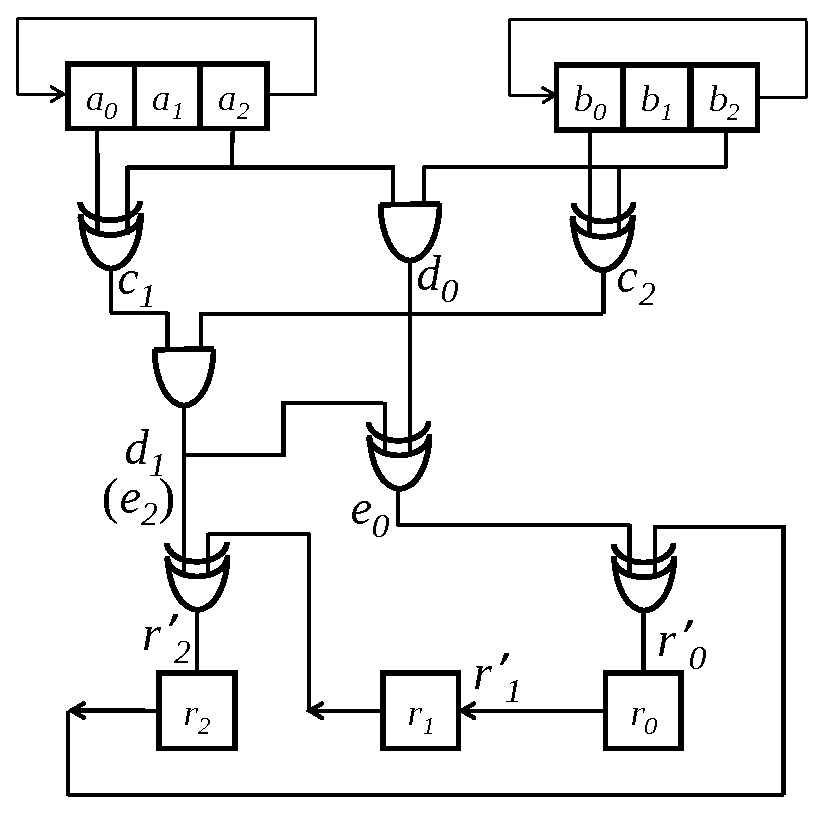
\includegraphics[width=2.25in]{./RH3.eps}
% \vspace{-0.2in}
\caption{A 3-bit RH-SMPO}
%\end{minipage}
\label{fig:RHmulti}}
\end{figure}

We follow  the typical sequential GF circuit model with word-level variables $A, B, R$
denoting {\it present states (PS)} and $A', B', R'$ denoting {\it next
  states (NS)} of the machine; where $A = \sum_{i=0}^{k-1} a_i \beta^{2^i}$
for the PS variables and $A' = \sum_{i=0}^{k-1} a_i'
\beta^{2^i}$ for NS variables, and so on.  Variables $R\ (R')$ correspond to those that 
store the result, and $A, B\ (A', B')$ store input operands. {\it E.g.,}
for a GF multiplier, $A_{init}, B_{init}$ (and $R_{init} =
0$) are the initial values (operands) loaded into the registers,  and
$R = \F(A_{init}, B_{init}) = A_{init} \times B_{init}$ is the final
result after $k$-cycles. Our approach aims to find this polynomial
representation for $R$.  

Each gate in the combinational logic is represented by a Boolean
polynomial. To 
this set of Boolean polynomials, we append the polynomials that define
the word-level to bit-level relations for PS and NS variables ($A =
\sum_{i=0}^{k-1} a_i \beta^{2^i}$). We denote this set of polynomials
as ideal $J = \langle 
f_1, \dots, f_s \rangle \subset \Fkk[x_1, \dots, x_d, R, R', A, A', B,
  B']$, where $x_1, \dots, x_d$ denote the bit-level (Boolean) variables
  of the circuit. The ideal of vanishing polynomials $J_0$ is also included, and
then the implicit FSM unrolling problem is setup for abstraction. 

The configurations of the flip-flops are the states of the
machine. {\it Since the set of states is a finite set of points, we
can consider it as the variety of an ideal related to the circuit
}. Moreover, since we are interested in
the {\it function encoded} by the state variables (over $k$-time
frames), we can {\it project this variety} on the word-level state
variables, starting from the initial state $A_{init}, B_{init}$.
Projection of varieties (geometry) corresponds to elimination ideals
(algebra), and can be analyzed via \Grobner bases. Therefore, we
employ a \Grobner basis computation with ATO: we use a {\it lex term
  order} with {\it bit-level variables} 
$>$ {\it word-level NS outputs} $>$ {\it word-level PS inputs}. This
allows to eliminate all the bit-level variables 
%(corresponding to the combinational logic and the state variables),
%so as to 
and derives a representation only in terms of words. 
Consequently, $k$-successive \Grobner basis computations implicitly
unroll the machine, and provide word-level algebraic $k$-cycle
abstraction for $R'$ as $R' = \F(A_{init}, B_{init})$. 

Algorithm
\ref{alg:modified} describes our approach.  In the algorithm, $from_i$
and $to_i$ are polynomial ideals whose varieties are the valuations of
word-level variables $R, A, B$ and $R',A',B'$ in the $i$-th iteration;
and the notation ``$\setminus$'' signifies that the $NS$ in iteration
$(i)$ becomes the $PS$ in iteration $(i+1)$. Line 5 computes the Gr\"obner 
basis with the abstraction term order.  Line 6 computes the elimination 
ideal, eliminating the bit-level variables and representing the set of 
reachable states up to iteration $i$ in terms of the elimination ideal. 
These computations are analogous to those of image computations performed in FSM reachability. 
%The forward image
%$to^{i}$ is computed using \Grobner bases with ATO.

\vspace{-0.1in}
\IncMargin{1em}
\begin{algorithm}[hbt]
\SetAlgoNoLine
\LinesNumbered
 \KwIn{Circuit polynomial ideal $J$, vanishing ideal $J_0$, initial
   state ideal $R (=0), \mathcal{G}(A_{init}), \mathcal{H}(B_{init})$} 

  $from_0(R,A,B) = \langle R, \mathcal{G}(A_{init}), \mathcal{H}(B_{init})\rangle$\;
  $i = 0$\;
  \Repeat{$i == k$}
  {
  	$i \gets i + 1$\;
%	$to^i(R',A',B') \gets$  $GB( \langle J_{ckt}, J_0,
%    from^{i-1}(R,A,B)\rangle )$ with abstraction term order\;
	$G \gets$GB$( \langle J + J_0+ from_{i-1}(R,A,B) \rangle
    )$ with ATO\;
	$to_i(R',A',B')\gets G\cap \mathbb F_{2^k}[R',A',B',R,A,B]$\;
	$from_i \gets to_i(\{R,A,B\}\setminus \{R',A',B'\})$\;
  }
\Return{$from_k(R_{final})$}
\caption {Abstraction via implicit unrolling for Sequential GF circuit
  verification}
\label{alg:modified}
\end{algorithm}
\DecMargin{1em}
\vspace{-0.1in}
\begin{Example}
\label{ex:RHSMPO}

We demonstrate our approach to verify the 3-bit RH-SMPO circuit of
Fig.\ref{fig:RHmulti}. The normal element $\beta$ in
$\mathbb{F}_{2^3}$ is known to be $\beta = \alpha^3$, where $\alpha$
is the primitive element. The circuit can be described with an ideal by translating
AND and XOR gates accordingly. For the first iteration:
\begin{align*}
J = &d_0+b_2\cdot a_2,
c_1+a_0+a_2,
c_2+b_0+b_2,
d_1+c_1\cdot c_2,\\
&e_0+d_0+d_1,
e_2+d_1,
r_0'+r_2+e_0,
r_1'+r_0,
r_2'+r_1+e_2,\\
&A+a_0\alpha^3+a_1\alpha^6+a_2\alpha^{12},
B+b_0\alpha^3+b_1\alpha^6+b_2\alpha^{12},\\
&R+r_0\alpha^3+r_1\alpha^6+r_2\alpha^{12},
R'+r_0'\alpha^3+r_1'\alpha^6+r_2'\alpha^{12};
\end{align*}
The last 4 polynomials are translated from the definition of word-level variables.
This represents ideal ``$J$" from line 5 in Algorithm
\ref{alg:modified}. ``$J_0$" is the ideal of vanishing polynomials in all bit-level
variables (e.g. $a_0^2-a_0$) and word-level variables (e.g. $A^8-A$). ``$from_{i-1}$"
% contains evaluation of PS word-level output in form of
% $R+\mathcal F(A,B)$. Since the definition of $A$ and $B$ changes after every iteration
% ($A',B'$ are different from $A, B$) and the multiplier's function only concerns about 
% initial value of $A,B$, we include the definition of $A_{init}, B_{init}$ into $from_i$:
represents the set of current states for iteration $i$.
In the first iteration, $from_0 = \{R, A_{init}+a_0\alpha^3+a_1\alpha^6+a_2\alpha^{12},
B_{init}+b_0\alpha^3+b_1\alpha^6+b_2\alpha^{12}\}$.

After the GB computation is performed with ATO, as line 6 in Algorithm \ref{alg:modified},
we find a polynomial in variables $R', A_{init}, B_{init}$ in $to_1 : 
R'+(\alpha^2) A_{init}^4 B_{init}^4+(\alpha^2+\alpha) A_{init}^4 B_{init}^2+(\alpha^2+\alpha) A_{init}^4 B_{init}+(\alpha^2+\alpha) A_{init}^2 B_{init}^4+(\alpha^2+\alpha+1) A_{init}^2 B_{init}^2+(\alpha^2) A_{init}^2 B_{init}+(\alpha^2+\alpha) A_{init} B_{init}^4+(\alpha^2) A_{init} B_{init}^2
$.

Line 7 in Algorithm \ref{alg:modified} simply replaces NS output $R'$ with PS output
$R$ in this example; so in second iteration $from_1 = \{
R'+(\alpha^2) A_{init}^4 B_{init}^4+(\alpha^2+\alpha) A_{init}^4 B_{init}^2+(\alpha^2+\alpha) A_{init}^4 B_{init}+(\alpha^2+\alpha) A_{init}^2 B_{init}^4+(\alpha^2+\alpha+1) A_{init}^2 B_{init}^2+(\alpha^2) A_{init}^2 B_{init}+(\alpha^2+\alpha) A_{init} B_{init}^4+(\alpha^2) A_{init} B_{init}^2
, A_{init}+a_2\alpha^3+a_0\alpha^6+a_1\alpha^{12},
B_{init}+b_2\alpha^3+b_0\alpha^6+b_1\alpha^{12}\}$. 

% By continue executing the loop,
Finally, after 3 iterations we obtain: $to_3 = \{ \mathbf{R'+A_{init}B_{init},}
~A_{init}+a_0'\alpha^3+a_1'\alpha^6+a_2'\alpha^{12},
~B_{init}+b_0'\alpha^3+b_1'\alpha^6+b_2'\alpha^{12}\}$
as the image. The final result is $from_3(R_{final}) = R_{final}+A_{init}\cdot
B_{init}$, which verifies the multiplier. 
\end{Example}

\subsection{Limitations: complexity of reduction (multivariate division)}
Although we gain success on verifying sequential GF multipliers, there are still problems when
doing implicit state enumerating on generic FSM. For example, when we tried to apply our approach
on ISCAS'89 benchmark s953 with 29 DFFs and 311 gates, RATO spent too much time on reducing
Spoly with ideal generators. By analyzing the process of polynomial reduction, we conjecture that
\begin{Conjecture}
Long chains of AND/OR gates will make polynomial reduction infeasible.
\end{Conjecture}

\begin{figure}[hbt]
\centering{
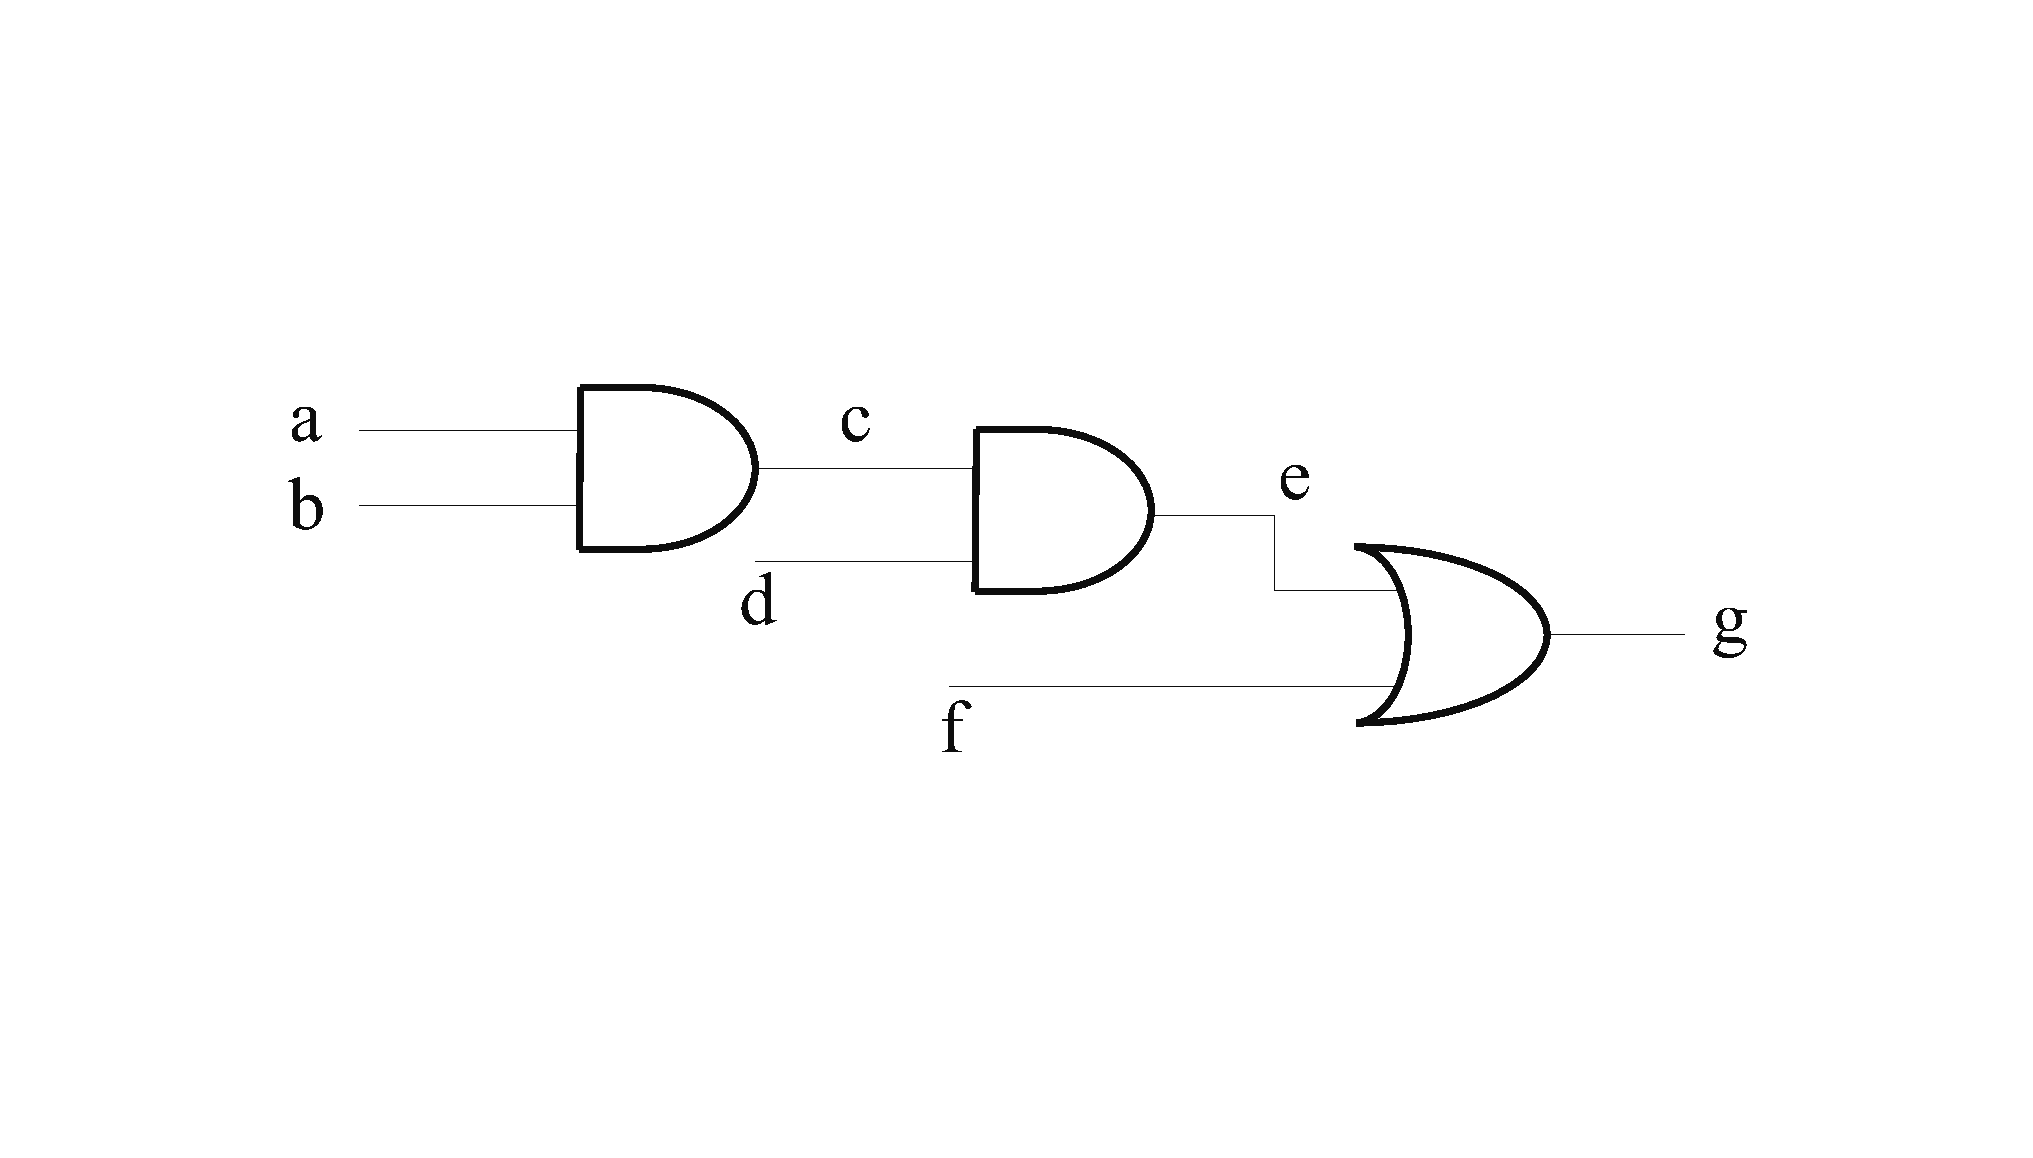
\includegraphics[scale=0.3]{./fig_chain.eps}
\caption{An example of AND-OR-gate chain}
\label{fig:chain}}
\end{figure}

\begin{Example}
Consider a chain (Fig.\ref{fig:chain}) of 3 gates: 2 AND gates and 1 OR gate. Write them in polynomials:
\begin{align*}
&h_1:g+ef+e+f\\
&h_2:e+cd\\
&h_3:c+ab
\end{align*}
Impose RATO: $g>e>c>\{a,b,d,f\}$. Reduce a simple polynomial $g$ with this set of polynomials:
$$g\xrightarrow{h_1}_{+} ef+e+f$$
$$g\xrightarrow{h_2}_{+} cdf+cd+f$$
$$g\xrightarrow{h_3}_{+} abdf+abd+f$$
We can conclude that:
\begin{itemize}
\item When divided by polynomial from XOR gate, the length of remainder will increase by 1 term;\\
\item When divided by polynomial from AND gate, the degree of remainder will increase by 1;\\
\item When divided by polynomial from OR gate, the length and degree of remainder will increase by 1.
\end{itemize}
Since all gate polynomials have leading term with degree 1, so increase of remainder degree means
iterations of division will at least increase by 1 (while there is still possibility to cancel multiple terms
at one time). Consider the querying time, a chain with AND/OR gates will blow up computational complexity of
reduction.

Sequential GF multiplier has only limited levels of gate chains (4 for RH-multiplier). Although the size of 
datapath is large, actual complexity for reduction is relatively low.
\end{Example}

To lower down the complexity of reduction, we can introduce a matrix-based technique named as "F-4 style reduction" \cite{F4reduce}. 
It can speed up the procedure dividing a low-degree polynomial with term-sparse polynomial ideal. 

Another option is to cut back the cost of each univariate division. Horner's expansion diagram (HED)\cite{alizadeh2010modular}
is a graphical method to turn operations such as uniting like terms to lower complexity DAG manipulations.

\begin{abstract}
This PhD dissertation proposal addresses the problem of sequential circuit verification at the word-level and is based on concepts derived from algebraic geometry. Analyzing the sequential circuits at word level is an efficient way
of {\it abstraction}, which may  lower the complexity of verification by efficient representation of the state-space. We propose to model the verification properties and the gate-level sequential circuit implementations over Galois fields of the type ${\mathbb{F}}_{2^k}$ by means of polynomial ideals and their canonical representations --- Gr\"obner bases --- at the level of $k$-bit words. Subsequently, techniques from algebraic geometry can be used to reason about the state-space by analyzing varieties of these ideals. 

We propose to apply these techniques to traverse a finite state machine (FSM) for reachability analysis at the word-level, and also to 
implicitly unroll sequential arithmetic circuits to verify their function. Moreover, as unsatisfiable (UNSAT) cores play an important role in modern abstraction-refinement techniques for verification, we propose to investigate a word-level analogue of the UNSAT core problem using the  Gr\"obner basis algorithm. The proposal will not only derive new algorithms and techniques, but will also consider efficient CAD implementations to target sequential equivalence and model checking problems. 
\end{abstract}

\chapter{Introduction} \label{ch:intro}
There is an ever-increasing need for secure communication within information 
technology. Security of sensitive information relies more and more heavily 
on encryption methodologies implemented in hardware by cryptographic 
circuits. One of the most prominent of these methodologies is Elliptical 
Curve Cryptography (\emph{ECC}), which provides more strength per encryption bit 
than other encryption methodologies.
The main building blocks of ECC hardware implementations 
are fast, \emph{custom-built Galois field arithmetic circuits}.
These circuits are notoriously hard to verify, yet their correctness is 
vitally important in critical applications. In \cite{crypto:bug_attacks}, 
for example, it is shown that a bug in the hardware could lead to the full 
leakage of the secret cryptographic key, which could compromise the entire
system. Thus, formal verification is imperative in Electronic Design 
Automation (\emph{EDA}) when dealing with cryptographic circuits.

To facilitate this verification, it is highly desirable to obtain a {\it word-level 
representation of the datapath of the ECC arithmetic block} from its 
bit-level implementation. Ideally, this abstraction should be {\it canonical},
as this allows the it to be directly applicable to equivalence checking. 
Such a canonical, word-level abstraction of the 
Galois field arithmetic block would not only make it easier to verify and 
reason 
about the cryptographic system as a whole, but also enable the use of 
higher level abstraction and synthesis tools. 
As arithmetic circuits are custom-designed, often modularly, using Galois field arithmetic blocks, 
the abstraction should also exploit the hierarchical nature of the circuitry.
Due to the modular circuit structure, abstraction of each arithmetic block
becomes the key in verification of the full circuit. 
Practical 
applications of ECC dictate a datapath of a minimum of $163$-bits, up to 
$571$-bits, as 
designated by the National Institute for Standards and Technology (NIST).
However abstraction of 
Galois field arithmetic circuits has been infeasible for data-paths beyond 
$16$ bits. 

This dissertation proposes an algebraic geometry based approach to abstract canonical, 
word-level representations of bit-level Galois field arithmetic circuits.
The approach is able to abstract representations
for circuits up to 571 bits in size, which is the largest NIST
standard for datapath size in ECC. 
Verification of circuits for which this abstraction has been computed is shown to 
be trivial; thus, the focus is on deriving the abstraction quickly and efficiently.
%Furthermore, we show how we can use these abstract representations to 
%perform improved formal verification of these circuits.

\section{Hardware Design and Verification Overview}
The typical design flow of a hardware system, 
as shown in Fig. \ref{fig:cadflow}, starts with a hardware system 
specification, which describes the necessary functions and parameters that 
the system must perform and adhere to. The specification is typically
modelled using a transaction-level model (\emph{TLM}), which describes 
communication details between large circuit modules. 
The TLM is then translated 
into a register-transfer-level (\emph{RTL}) description, which is composed of abstracted, 
interconnected circuit blocks that compose the entire system. RTL is 
typically implemented 
in hardware description languages (\emph{HDL}) such as Verilog and VHDL, 
which are the most popular choices in the industry.
Next, the RTL is optimized and converted into a \emph{netlist}, i.e. a large 
collection of small physical blocks (MOSFET, Boolean logic gates, etc.) and 
the inter-connections (wires) between them. 
Lastly, the netlist is further optimized and then mapped onto a physical space 
on a chip, which is then sent off for fabrication. This entire design flow
is automated by Computer-Aided Design (\emph{CAD}) tools. 

{
\begin{figure}[h]
\centerline{
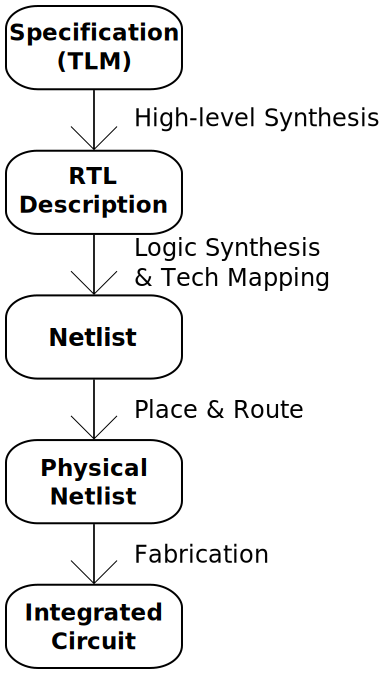
\includegraphics[width=0.5\textwidth]{./figures/designFlow}
}
\caption{Typical hardware design flow.}
\label{fig:cadflow}
\end{figure}
}

%\subsection{The Hardware Verification Imperative}
When moving from one abstraction level of the hardware design process to the 
next, an important issue arises: how can one ensure that the functionality of 
the optimized design matches original spec? 
Bugs in hardware design which are 
not caught early can have costly effects later, such as the need for a 
redesign. Bugs in arithmetic circuits can be especially catastrophic.
One infamous example is the 1994 floating point division (FDIV)
bug that affected the Intel Pentium chip \cite{nicely:FDIV}, 
and subsequently cost the company \$475 million because it was  
discovered after the chip's release. In another more fatal case, during the
Gulf war, an American Patriot Missile battery failed to intercept an incoming
enemy missile due to an arithmetic error \cite{arnold:patriot}.
Since hardware bugs can have significant consequences, 
there has been extensive work in field of hardware verification to find and
eliminate bugs prior to fabrication.

The two main methodologies used in hardware verification are simulation and 
formal verification. \emph{Simulation} checks correctness by applying exhaustive 
assignments to the circuit inputs and verifying correctness of the output. 
This ensures that the circuit performs as designed under all possible 
inputs. Such exhaustive testing is quite effective for smaller circuits. 
However, as the size of the circuit increases, it becomes 
computationally infeasible to simulate all possible test vectors. This is the 
case with Galois field arithmetic circuits, which are commonly very large in 
real-world applications. Often for such large circuits, simulations of a smaller and more 
manageable subset of test vectors are employed to catch bugs. While these tests
can increase confidence in the correctness of the design,  
{\it they do not guarantee correctness} since every data-flow of the design hasn't
been analyzed.
%Such is the case with large Galois field arithmetic circuits, so we instead 
%focus on formal verification. 

\section{Formal Verification}
Instead of simulating input vectors, \emph{formal verification} utilizes 
mathematical theory to reason about the correctness of hardware designs.
%which overcomes some limitations of simulation. 
Formal verification has two main forms: property checking and equivalence 
checking. 

{\it Property checking} (or property verification) verifies
that a design satisfies certain given properties. Property checking is done mainly 
in the form of theorem proving, model checking, or approaches which 
combine the two.
\begin{enumerate}
\item \emph{Theorem proving} \cite{theoremproving:91} requires the existence of
mathematical descriptors of the specification and implementation of the 
circuit. Theorem provers apply mathematical rules to these descriptors to
derive new properties of the specification. In this way, the tool can reduce
a proof goal to simpler sub-goals, which can be automatically verified.
However, generating the initial proof-goal requires extensive guidance from
the user, so there is an overall lack of automation in theorem 
proving.
\item \emph{Model checking} \cite{modelcheck:99} is an approach
to verifying finite-state systems where specification 
properties are modeled as a system of 
logic formulas. The design is then traversed to check if the 
properties hold. If the design is found to violate a
particular property, a counter-example is generated which exercises the
incorrect behavior in the design. Such counter-examples allow the designer
to trace the behavior and find where the error in the design lies.
Modern model checking techniques use the result to automatically refine
the system and perform further checking.
These tools are typically automated, and thus have found widespread 
use in CAD tool suites.
\end{enumerate}

{\it Equivalence Checking} verifies that two different representations of
a circuit design have equivalent functionality. An example of equivalence
checking as it applies to the hardware design flow is shown in
Fig. \ref{fig:equivflow}.

{
\begin{figure}[h]
\centerline{
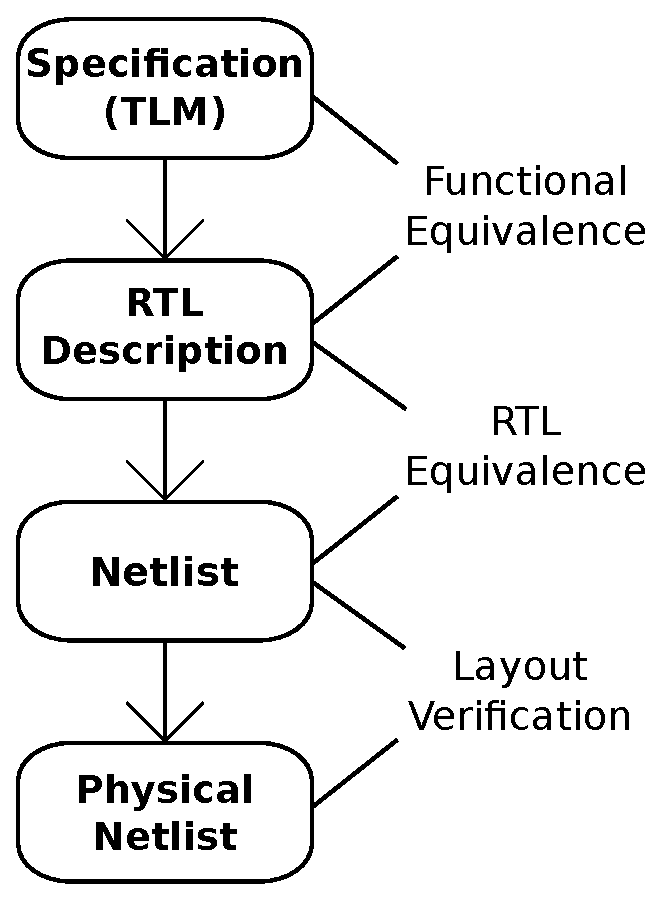
\includegraphics[width=0.5\textwidth]{./figures/designVerification}
}
\caption{Equivalence checking as applied to the hardware design flow.}
\label{fig:equivflow}
\end{figure}
}

There are two major
equivalence checking techniques: graph-based
and satisfiability-based.
\begin{enumerate}
\item \emph{Graph-based} techniques construct a canonical graph 
representation, such as a Binary Decision Diagram (\emph{BDD}) or one of
its many variants, of each circuit. A linear comparison is then conducted to 
determine whether the two graphs are isomorphic. Since the graph 
representation is canonical, the graphs of the two circuits will be 
equivalent if and only if the circuits perform the same function.
\item \emph{Satisfiability} techniques construct a miter of the two circuits,
typically in a graph such as an And-Inverter graph (\emph{AIG}). A
\emph{miter} is a combination of the two circuits with one bit-level output, which 
is only in a "1" state when the outputs of the circuits differ given 
the same given 
input, as shown in Fig. \ref{fig:miter}. 
A satisfiability (\emph{SAT}) tool \cite{csat} 
is then employed to simplify the graph and find a solution to the miter, 
i.e. find an input for which the 
miter output is "1". If a solution is found, this solution acts as a 
counter-example of when the circuit outputs differ; otherwise the circuits
are functionally equivalent.
\end{enumerate}


{
\begin{figure}[h]
\centerline{
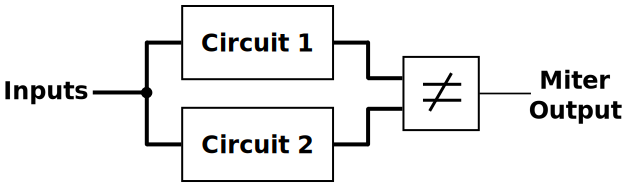
\includegraphics[width=0.8\textwidth]{./figures/betterMiter}
}
\caption{A miter of two circuits.}
\label{fig:miter}
\end{figure}
}

%\subsection{Computer-Algebra Based Formal Verification}
Certain formal verification methods use \emph{computer-algebra} and \emph{algebraic
geometry} techniques based on mathematical theories.
Unlike SAT-based verification, modern algebraic geometry 
techniques do not explicitly solve the constraints to find a solution; 
rather, they reason about the presence or absence of solutions, or explore
the geometry of the solutions.
These methods \cite{Avrunin:CAV} \cite{condrat-tacas07} \cite{gbverify:2007} 
transform the circuit design into a polynomial system. Typically, this system
of polynomials is then used to compute a Gr\"obner basis \cite{gb_book}. 
Computation of Gr\"obner bases allows for 
the easy deduction of important properties of a polynomial system, 
such as the presence or absence of 
solutions. These properties are then leveraged to perform 
verification. Unfortunately, such a computation 
has been shown to be doubly 
exponential in the worst case, and thus these methods have not been 
practical for real-world applications. However, recent
breakthroughs in computer-algebra hardware verification have shown
that it is possible to overcome the complexity of this computation while
still utilizing the beneficial properties of a Gr\"obner bases
\cite{lv:phd}.

\section{Importance of Word-level Abstraction}
Most formal verification techniques can benefit from word-level abstractions 
of the circuits they verify.
Abstraction is defined as state-space reduction, i.e{\text . }abstraction
reduces state-space by mapping the set of states of a system to a smaller 
set of states. Because the new representation contains fewer states, it
is easier to comprehend and thus easier to use. 
Word-level abstraction focuses specifically on abstracting a word-level
representation of a circuit out of a bit-level representation. For example,
a bit-level representation of an integer multiplier is represented by a
collection of Boolean inputs and outputs, whereas a word-level
abstraction hides the underlying logic and represents the circuit as two 
integer inputs and one integer output, e.g. $Z=A\cdot B$. As the bit-size of the
multiplier increases, the logical implementation of the multiplier grows (typically
exponentially) while the word-level abstraction stays the same.

Word-level abstractions have a wide variety applications in formal 
verification. Theorem proving techniques can leverage abstraction as an 
automatic decision procedure or as a canonical reduction 
engine. For example, since RTL is composed of circuit blocks that represent 
the underlying circuit, RTL verification methods can exploit 
abstractions of these blocks.
This is seen in the following RTL verification methods:
\begin{itemize}  
\item Model checking \cite{kroening:model}, 
where an approximation abstraction of RTL blocks is generated and then 
refined.
\item Graph-based equivalence 
checking \cite{WLS} \cite{arditi:bmd}, where abstraction methods are used
to generate a canonical word-level graph representation of the circuit.
\item Satisfiability-based equivalence checking \cite{lpsat}, where 
abstractions are used identify symmetrics and similarities in order to 
minimize the amount of logic that is sent to the 
SAT tool. 
\end{itemize}

Other equivalence checking techniques that employ abstractions 
include satisfiability modulo theory ({\it SMT}) techniques \cite{boolector} \cite{bryant:tacas07}, 
which are similar to SAT except they operate on higher-level data
structures (integers, reals, bit vectors, etc.), as well as 
constraint solving techniques \cite {ms:research} \cite{tew:iccad08}.
In general, RTL equivalence checking approaches would ideally maintain a 
high-level of abstraction while still retaining sufficient lower-level 
functional details  (such as bit-vector size, precision, etc) 
\cite{gupta_survey}.

Word-level hardware abstractions also have applications in RTL and datapath 
synthesis \cite{demicheli:iccad_98} \cite{demicheli:dac_99}
\cite{demicheli:tcad_03}. 
Abstractions of circuits allow for design reuse, which allows for tool-automated 
synthesis of larger circuit blocks.
Since hardware design specifications tend to be word-level, synthesis tools 
can use these larger circuit blocks to generate and optimize the
datapaths and create the RTL of the system. Thus, in order for a circuit to 
be used by these automated synthesis tools, its word-level abstraction must
be known.

Finally, abstractions can also be applied to detect malicious 
modifications to a circuit, potentially inserted as a hardware trojan horse.
Hardware trojans, a relatively new security concern in the hardware 
industry, use certain techniques to add incorrect behavior to a 
design. 
This behavior is only activated under certain rare circumstances that only 
the mal-intent designer has knowledge of.
The behavior is purposely hidden and is very difficult to encounter during 
simulation of the design. A manufactured chip with a subsystem 
that contains a hardware trojan could compromise the entire system in which 
it is used.
In some hardware trojan cases, formal verification techniques may be applied 
to catch a bug in a design and provide a counter-example which exercises it. 
However, it can be difficult to tell whether the bug in the design was 
introduced intentionally of not. On the other hand, word-level abstractions 
of bit-level circuits {\it effectively reverse-engineer the true function 
implemented by the circuit}, which could be used to determine the designer's 
true intention.

\section{Dissertation Objective, Motivation, and Contributions}
This dissertation focuses on abstracting a canonical, 
word-level representation of hardware (bit-level) implementations of 
combinational circuits. The proposed technique is a full abstraction solution which can be 
applied to any arbitrary acyclic combinational circuit. 
It is particularly efficient when applied to Galois field arithmetic circuits.
Using this technique, if the abstraction of the circuit's implementation and its
specification are found, they can be easily compared to determine equivalence.
Implementation of a custom software tool, developed to compute the abstractions, is
also described.

\subsection{Motivating Application}
The motivation for this work comes from applications of Galois field 
arithmetic circuits in elliptical curve cryptography ({\it ECC}) hardware systems.
The main operations of encryption, decryption, and 
authentication in ECC rely on operations performed on elliptic curves, which 
are implemented in hardware as polynomial functions over Galois fields. 
To be applicable in real-world situations, ECC data-paths
should be a minimum of $163$-bits wide, which is the minimum NIST standard, 
up to a recommended size of $571$-bit operand widths. Many non-ECC cryptosystems
have datapaths on the order of $1000$-bits.

A Galois field arithmetic circuit with a datapath size of $k$ 
is built as a Boolean function: $\mathbb{B}^k \rightarrow \mathbb{B}^k$. 
This function is mapped to an operation 
$f:\mathbb{F}_{2^k} \rightarrow \mathbb{F}_{2^k}$ 
over the Galois field $\mathbb{F}_{2^k}$. 
These circuits are custom-built, modular
systems which cannot be synthesized due to their complex nature. Thus, 
formal verification is needed to ensure they operate correctly.

Recent computer-algebra based formal verification techniques have been
able to perform verification of Galois field arithmetic circuits with
a datapath size up to $163$-bits \cite{lv:phd}. Word-level abstractions 
of Galois
field arithmetic circuits could be used to further improve these formal 
verification techniques to allow for verification of larger circuits, as
well as provide the other benefits of word-level abstraction.
However, there is currently no technique for computing word-level 
abstractions of Galois field circuits of any practical size.

{
\begin{figure}[h]
\centerline{
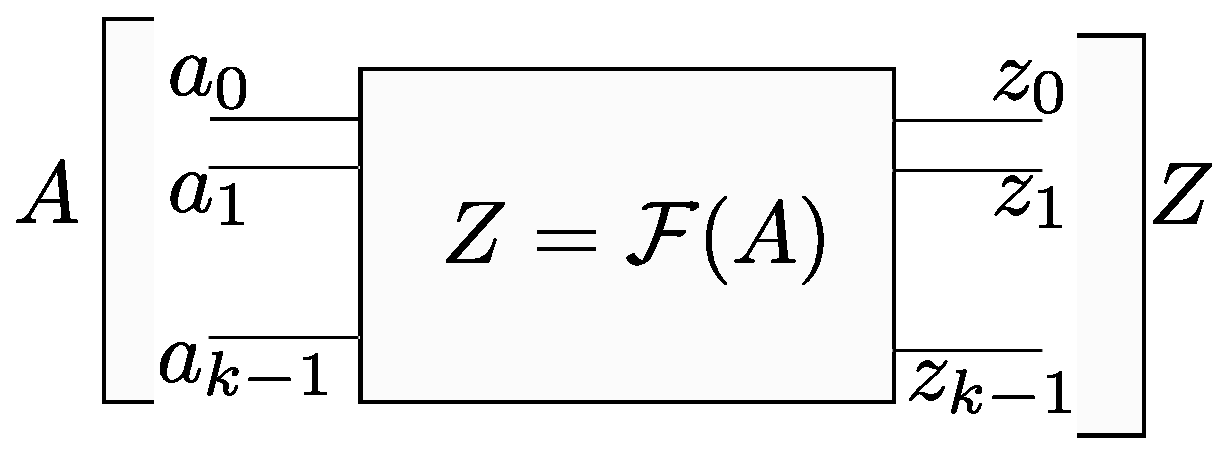
\includegraphics[width=0.5\textwidth]{./figures/interpolate}
}
\caption{Circuit with $k$-bit input $A$ and $k$-bit output $Z$. 
Abstraction to be derived as $Z=\Func(A)$.}
\label{fig:abstractA_Z}
\end{figure}
}

While the motivation comes from the need to verify Galois field arithmetic
circuits, the presented approach can be generalized to be applicable to any
combinational acyclic circuit.
Any such circuit with a $k$-bit input $A$ and a $k$-bit output $Z$, such
as the one shown in Fig. \ref{fig:abstractA_Z}, computes 
$f: \mathbb{B}^k \rightarrow \mathbb{B}^k$ and can thus be analyzed as the
function $f: \Fkk \rightarrow \Fkk$. Over $\Fkk$ this function can be 
represented as the polynomial $Z=\Func(A)$. This is trivially generalized
when there are multiple $k$-bit inputs $A_1,A_2,\dots,A_i$, i.e. $Z=\Func(A_1,\dots,A_i)$.
Now assume the word-size of the input differs from the output, that is the circuit
computes $f: \mathbb{B}^m \rightarrow \mathbb{B}^n$ for $m \neq n$. This can 
be represented as a function over Galois fields as $f: \F_{2^m} \rightarrow \F_{2^n}$.
This function can be analyzed over the field $\Fkk$ such that $\Fkk \supset \F_{2^m}$ 
and $\Fkk \supset \F_{2^m}$, where $k=LCM(m,n)$.

\subsection{Dissertation Contributions}
To solve the problem of word-level abstraction, this dissertation proposes 
a full solution consisting of three main contributions.

\begin{enumerate}
\item A theory for finding the word-level abstraction from a bit-level circuit over Galois fields is created.
The given bit-level circuit implementation is modelled as a system of
polynomials over the field.
This theory is derived using techniques from computer-algebra, notably the theory of
\Grobner basis \cite{pruss:iwls13}.
\item Using this theory, new algorithms based on symbolic computation are developed to 
derive the word-level abstraction. The algorithms are designed to be applicable to 
industry-size arithmetic circuits over Galois fields \cite{pruss:dac14}\cite{sun:date15}.
A complexity analysis of the algorithmic approach is also presented. Furthermore, the
approach is also generalized to make it applicable to arbitrary combinational circuits.
Finally, we show how the approach can be used to exploit the hierarchical structure of
large Galois field multipliers designed over composite fields.
\item A custom software tool implementation of the algorithmic approach is described, including
an analysis of efficient data structures designed for this purpose \cite{pruss:tcad15}.
\end{enumerate}

Experiments show that the proposed solution can abstract canonical, word-level, 
polynomial representations of Galois field arithmetic circuits up to $1024$-bits in
size, while other contemporary approaches are infeasible beyond a $32$-bit designs.


%an 
%approach based on computer-algebra, algebraic geometry - notably the theory of
%{\it Gr\"obner bases} \cite{gb_book} \cite{buchberger_thesis}.
%and {\it elimination ideals} \cite{ideals:book}, as our approach for 
%abstracting canonical word-level representations from bit-level Galois 
%field arithmetic circuits. 
%Computer-algebra techniques easily integrate with 
%Galois field theory and allow for polynomial abstraction of the circuit over 
%the field itself. Thus, if the circuit computes a function over some field $
%\mathbb{F}_{2^k}$, the resulting abstraction is a word-level polynomial 
%function over the same field $\mathbb{F}_{2^k}$. 

%The given bit-level circuit implementation is first modeled as a system of
%polynomials over the field. Using the theory of elimination ideals, we 
%derive an elimination term ordering and prove that by using this ordering we 
%can obtain a canonical word-level representation of a circuit by 
%computing a Gr\"obner basis of the polynomials. However, complexity 
%of the computation of a Gr\"obner basis proves to be prohibitive for circuits
%of practical size. Therefore, we employ a select sub-set of computations 
%from the Gr\"obner basis theory to overcome this complexity and obtain the
%abstraction. We prove that this simpler computation can be 
%performed via a polynomial reduction process, and engineer a custom 
%verification tool for this purpose. Using this approach, we are able to 
%successfully 
%abstract word-level representations of Galois field arithmetic circuits up 
%to $571$-bits, which is the {\it largest recommended NIST standard} for ECC.


\section{Dissertation Organization}
The rest of this dissertation is organized as follows. Chapter
\ref{ch:prev} reviews previous applicable work and highlights their
drawbacks with respect to the canonical, word-level abstraction problem. 
Chapter \ref{ch:prelim} describes the properties of Galois fields, 
$\mathbb{F}_{2^k}$, and explains the process of constructing them.
It also describes how to design arithmetic circuits over such fields, their 
complexities, and the role of these circuits in Elliptic Curve Cryptography.
Chapter \ref{ch:ideals} provides a theoretical background of 
computer-algebra and Gr\"obner bases and explains their application
to Galois fields. 
Chapter \ref{ch:abstract} describes an approach to abstract 
word-level polynomial representations of combinational circuits using a 
Gr\"obner basis computation.
Chapter \ref{ch:improv} improves on this word-level abstraction approach to 
make it applicable to much larger circuits.
Chapter \ref{ch:generalize} generalizes the abstraction approach to make
it applicable to circuits with varying operand word-lengths. It also describes how the 
approach can take advantage of the hierarchy of arithmetic circuits designed over
composite fields.
Chapter \ref{ch:implement} describes the implementation details of a 
custom abstraction tool and gives experimental results of
abstracting large Galois field multiplier circuits.
Chapter \ref{ch:concl} concludes the dissertation and outlines potential future 
research for continuation of this work. 

%\input{myformulae.tex}


\section{Preliminaries}

\subsection{FSM model for sequential circuits}
A finite state machine (FSM) is a mathematical model of computation for designing and analyzing sequential logic 
circuits. If a FSM's primary outputs depend on primary inputs and present state inputs, it is named as a \textit{Mealy machine};
the formal definition is as follows:
\begin{Definition}
A Mealy machine is an $n$-tuple $\mathcal M = (\Sigma,O,S,S^0,\Delta,\Lambda)$ where
\begin{itemize}
\item $\Sigma$ is the input label, $O$ is the output label;
\item $S$ is the set of states, $S^0\subseteq S$ is the set of initial states;
\item $\Delta:\ S\times\Sigma\to S$ is the next state transition function;
\item $\Lambda:\ S\times\Sigma\to O$ is the output function.
\end{itemize}
\end{Definition}
The other kind of FSM is \textit{Moore machine}, its difference from Mealy machine is that
its primary outputs only depend on the present states, i.e. the output function is defined as
$$\Lambda:\ S \to O$$
Typical sequential circuits can be depicted as Fig.\ref{fig:seqmodel}(a). Primary inputs
$x_1,\dots,x_m \in \Sigma$, and primary outputs $z_1,\dots,z_n\in O$. Signals $s_1,\dots,s_k$ 
are present state (PS) variables, $t_1,\dots,t_k$ are next state (NS) variables.
We can define 2 $k$-bit words denoting the PS/NS variables as there are $k$ flip-flops
in the datapath: $S = (s_1,\dots,s_k), ~T=(t_1,\dots,t_k)$. Transition function
at bit level are defined as $\Delta_i: t_i = \Delta_i(s_1,\dots,s_k,x_1,\dots,x_m)$.
\begin{figure}[hbt]
\centering{
%\begin{minipage}{12cm}
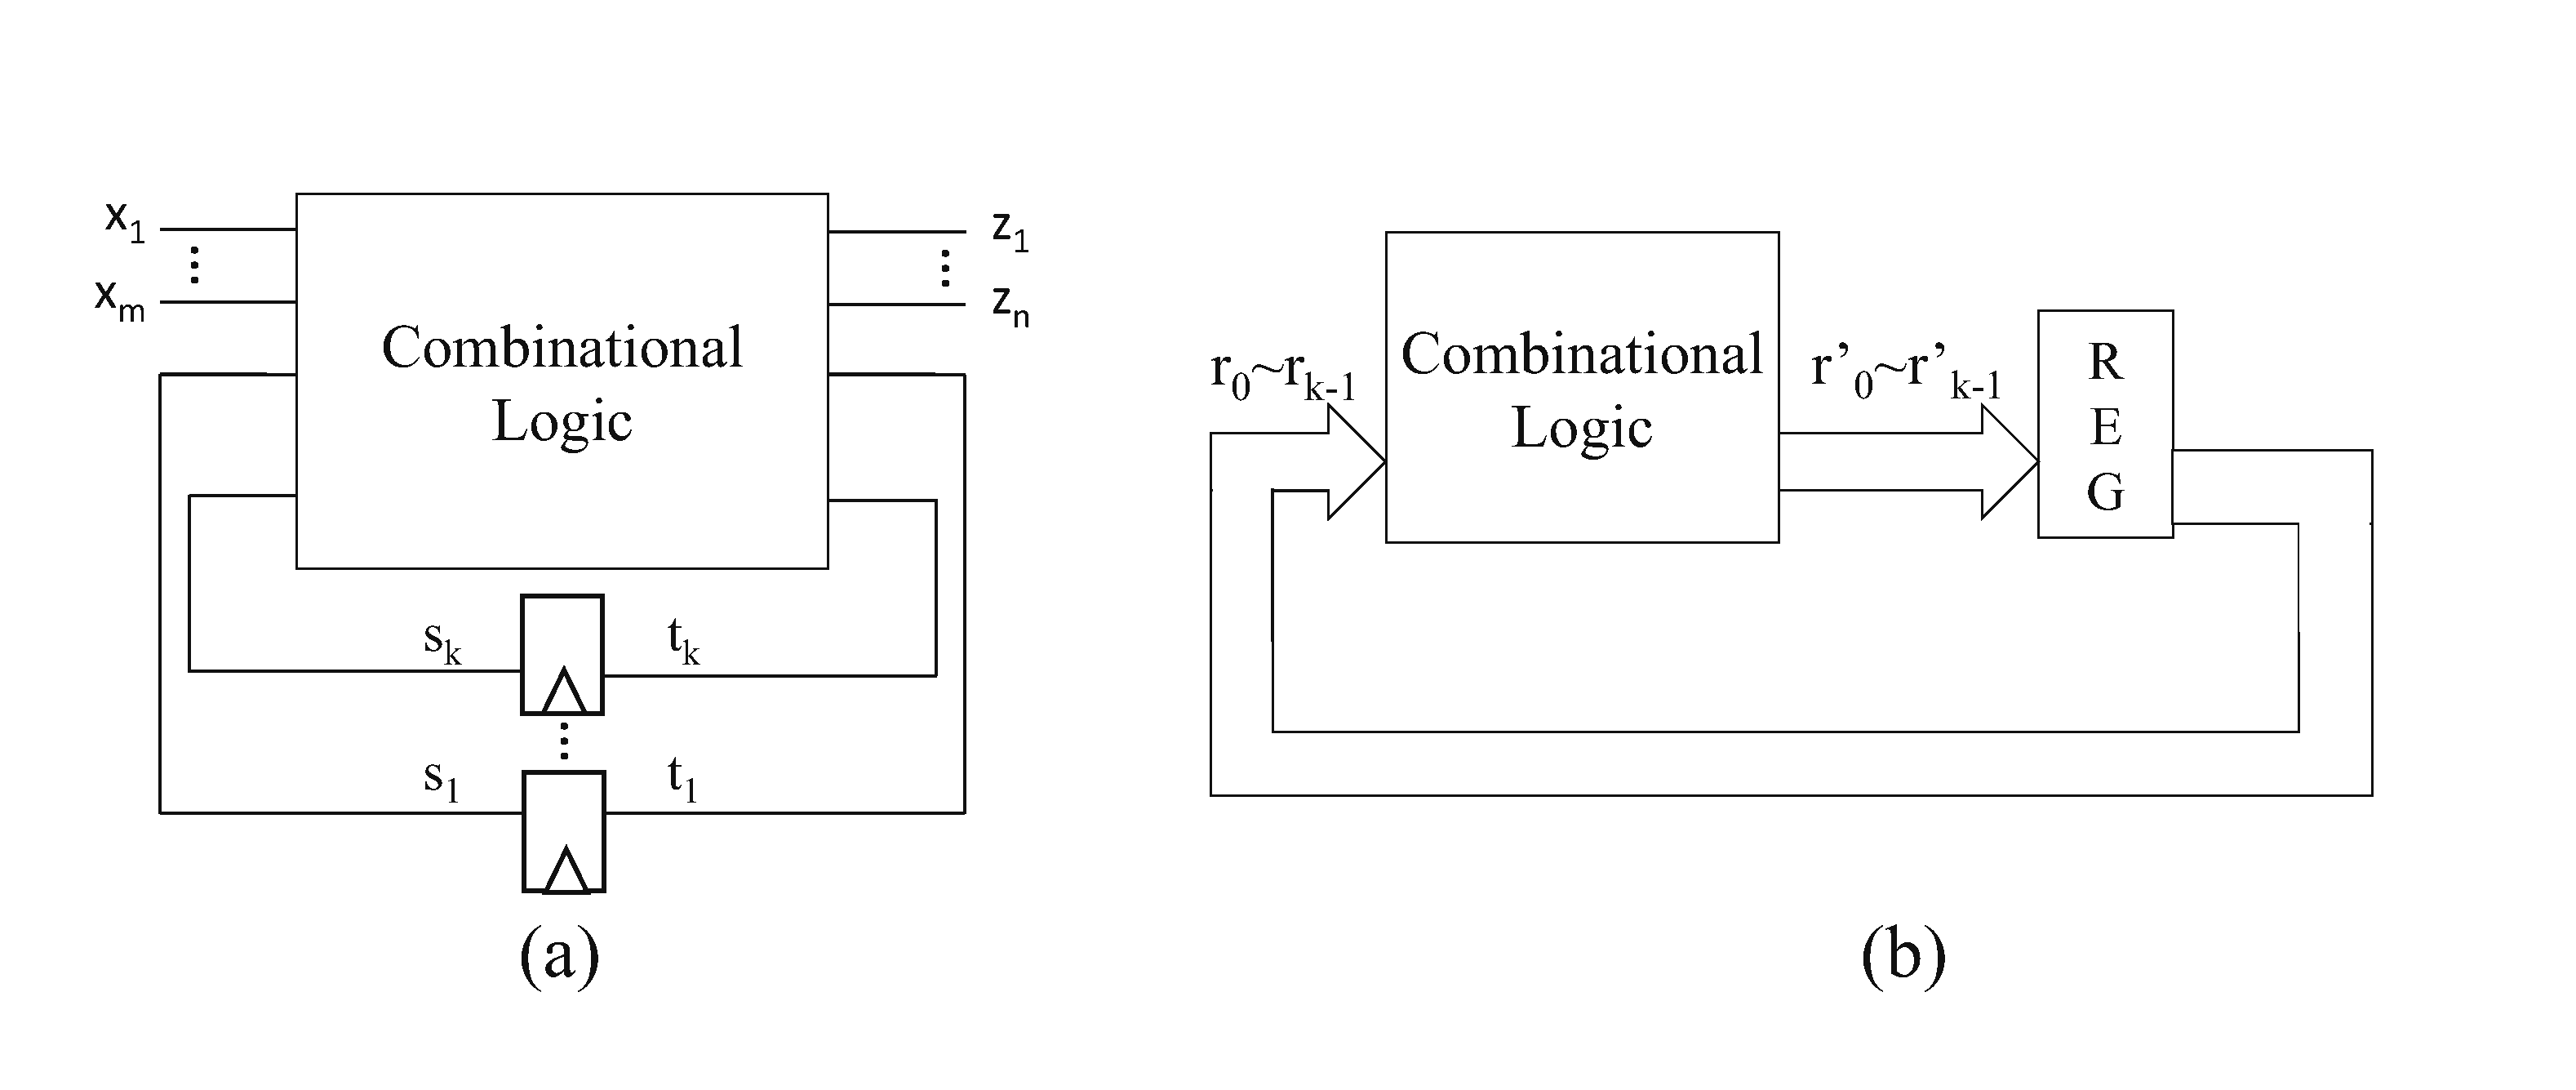
\includegraphics[width=3.5in]{./seqmodel.eps}
% \vspace{-0.2in}
\caption{FSM models of sequential circuits}
%\end{minipage}
\label{fig:seqmodel}}
\end{figure}
In some cases, arithmetic computations are implemented as Moore machines where input operands
are loaded into register files $R$ and the FSM is executed for $k$ clock cycles.
We can simplify them to the model in Fig.\ref{fig:seqmodel}(b).

\subsection{Commutative algebra and algebraic geometry preliminaries}
A {\bf field} $\mathbb{F}$ is a set of elements, including 0 and 1 (unity),
allowing for associative and commutative addition and multiplication;
and every non-zero element has a multiplicative inverse.  A {\bf
  finite field} or {\bf Galois filed} is a field with a finite number
($q$) of elements, and is denoted by $\Fq$, where $q=p^k$ is a power of
a prime integer $p$. In our work, $q = 2^k$ for
a given $k$, where $k$ represents the datapath (bit-vector)
word-lengths, or the number of memory elements (state registers) in
finite state machines. 

Let the field $\mathbb{F}_2 = \{0, 1\} ~(\equiv \B)$, and let
$\mathbb{F}_2[X]$ denote the set (ring) of all univariate polynomials
in variable $X$ with coefficients from $\mathbb{F}_2$. Then, the
Galois field $\Fkk$ is constructed as $\Fkk = \mathbb{F}_2[X] \pmod{
  P(X)}$, where $P(X)$ is an irreducible polynomial over
$\mathbb{F}_2$. Let $\alpha$ be a root of the irreducible polynomial
$P(X)$, i.e. $P(\alpha) = 0$. Any element $A \in \Fkk$ can be
represented as $A = \sum_{i=0}^{k-1} a_i \alpha^i$, where $a_i \in
\mathbb{F}_2$. The field $\Fkk$ is therefore, a $k$-dimensional {\it
  extension} of the base field $\mathbb{F}_2$: so,  $\mathbf{\Fkk \supset
\mathbb{F}_2}$. Consequently, all operations of addition and
multiplication in $\Fkk$ are performed modulo the irreducible
polynomial $P(\alpha)$ and coefficients are reduced modulo 2.  

Boolean variables in field $\mathbb B$ can be easily mapped to
elements in $\mathbb F_2$. Since $\mathbb F_2 \subset \Fkk$, these 
%Namely $k$-bit Boolean bit-vector defined
%over Boolean ring $\mathbb B^k$ can also be mapped uniquely  to $\Fkk
%= \mathbb F_2[x_1,\dots,x_k]$. 
Boolean operators are interpreted as functions over $\Fkk$ (where $+$
and $\cdot$ are addition and multiplication performed modulo 2): 
\begin{align*}
&a\land b \to a\cdot b\\
&a\oplus b \to a+b\\
&\neg a \to 1+a\\
&a \bar{\oplus} b \to 1+a+b\\
&a \lor b \to a+b+a\cdot b
\end{align*}

Using these mappings we can write Boolean functions in form of
polynomials over $\mathbb F_2\subset \Fkk$. 
These concepts provide a mechanism to represent and
manipulate both bit-level ($\mathbb{F}_2$) and $k$-bit word-level
constraints {\bf in one unified mathematical domain $\Fkk$ --- a
  concept we   exploit for abstraction. }
  Consider Ex.\ref{ex:motiv},
polynomials for transition functions (bit-level outputs) $f_1,f_2$
are over $\mathbb F_2$, i.e. $f_1,f_2\subseteq \mathbb F_2 \subset \Fkk$,
and polynomials containing word-level variables $f_3,f_4,f_5 \subseteq \Fkk$.
All polynomials belong to unified domain $f_1,f_2,\dots,f_5 \subseteq \Fkk$.

It is well-known that every Boolean mapping between $k$ dimensional
Boolean spaces $f: \B^k \rightarrow \B^k$ can be construed as a
function over Galois fields $f: \Fkk \rightarrow \Fkk$. Moreover,
every function $f: \Fkk \rightarrow \Fkk$ is a polynomial function: 
i.e. $f$ can be represented by way of a unique, minimal, canonical
polynomial $\F(X)$, and the work of \cite{timDAC} shows how to
efficiently derive such polynomial representations from circuits ---
another concept that makes our approach feasible. 


We represent Boolean circuits by way of polynomials over
$\Fkk$. If we take indeterminates $x_1,x_2,\dots,x_n$, an arbitrary
combination of their finite product  
$x_1^{d_1}\cdot x_2^{d_2}\cdots x_n^{d_n}, d_i\geq 0$ 
is a {\bf monomial}. A {\bf polynomial} $f = c_1 X_1 + c_2 X_2 + \dots
+ c_t X_t$ is a finite sum of terms, where $c_1, \dots, c_t$ are
coefficients and $X_1, \dots, X_t$ are monomials. The set of {\it all}
such polynomials with coefficients from $\Fkk$ forms a {\bf
  multivariate polynomial ring} denoted $\Fkk[x_1,\dots,x_n]$. 
A monomial ordering $X_1 > X_2 \dots > X_t$ is imposed on the
polynomials to process them systematically. Then, $LT(f) = c_1 X_1,
LM(f) = X_1$ denote the leading term and the leading monomial of $f$,
respectively. 


Multivariate polynomial division will play a key role in our
algorithmic techniques. Division is implemented as {\it cancellation
  of terms.} Given polynomials $f, g$, if $cX$ is a term in
$f$ that is divisible by $LT(g)$, then $f \xrightarrow{g} r$ denotes a
one-step reduction (division) of $f$ by $g$, resulting in remainder $r
= f - {{cX} \over {LT(g)}} \cdot g$. This has the effect of cancelling
the term $cX$ from $f$. 
\begin{Example}
\label{ex:multidiv}
If $f = e + cd$ and $g = c + ab$,
then the term $cd$ in $f$ can be canceled by $LT(g) = c$: $r = f - {cd
  \over c} g = e + abd$. 
\end{Example}
  Similarly, $f$ reduces to $r$ modulo the set
of polynomials $F = \{f_1, \dots, f_s\}$, denoted $f \stackrel{F}
{\textstyle   \longrightarrow}_+ r$, such that no term in $r$ is
divisible (cancellable) by the $LT(f_i)$ of any polynomial in $ f_i
\in F$.    


In verification, we have to analyze the {\it solutions to a
set of polynomials.} The set of all solutions to a system of
polynomial equations $f_1 = \dots = f_s = 0$ is defined as the affine variety:
\begin{Definition}
Given a set of polynomials $f_1,\dots,f_s$ over ring $\mathbb F_q[x_1,\dots,x_n]$, their 
{\bf affine variety} 
$$V(f_1,\dots,f_s) = \{(a_1,\dots,a_n)\in  (\mathbb F_q)^n |
f_1(a_1,\dots,a_n) = \cdots = f_s(a_1,\dots,a_n) = 0\}$$ 
\end{Definition}

Generally we can find many sets of polynomials with the same variety, which are linear combinations
of given set of polynomials. This set is defined as follows:
\begin{Definition}
{\bf Ideal of Polynomials:} Let $f_1,f_2,\dots,f_s\in \mathbb F[x_1,\dots,x_n]$.
Define an ideal
$$J = \langle f_1,f_2,\dots,f_s\rangle = \{f_1\cdot h_1 + f_2\cdot h_2 +\cdots + f_s\cdot h_s : h_1,\dots,h_s\in \mathbb F[x_1,\dots,x_n]\}$$
We call $J = \langle f_1,f_2,\dots,f_s\rangle$ an ideal generated by $f_1,\dots,f_s$ and these polynomials 
the {\bf generators} of ideal $J$.
\end{Definition}
% On the other hand, if given another polynomial $f$, we need to judge whether it belongs to $J$.
A practical problem is: given an ideal $J = \langle f_1,f_2,\dots,f_s\rangle$ and a polynomial $f$,
we need to check if the variety of $J$ can make the evaluation of $f$ equal to 0, i.e. $f$ vanishes on $V(J)$.
This problem is usually described as ideal membership checking problem.
\begin{Definition}
{\bf Ideal membership:} Let $f_1,f_2,\dots,f_s\in \mathbb F[x_1,\dots,x_n]$, and $J = \langle f_1,f_2,\dots,f_s\rangle$
be an ideal over ring $\mathbb F[x_1,\dots,x_n]$. If 
$$f = f_1h_1 + f_2h_2 + \cdots + f_sh_s$$
then $f\in J$.
\end{Definition}

An ideal may have many generating sets. For example, we may have different set of polynomial generators denoting
the same ideal, where they have the same variety: $\langle f_1,\dots,f_s\rangle = \langle h_1,\dots,h_r\rangle
= \langle g_1,\dots,g_t\rangle$ such that $V(f_1,\dots,f_s) = V(h_1,\dots,h_r) = V(g_1,\dots,g_t)$.
Therefore a canonical representation of an ideal is needed, which leads to the concept of Gr\"obner bases.

\begin{Definition}
The set $G = \{g_1, \dots,
g_t\}$ is called a \textbf{\Grobner basis} of $J$ if and only if the
leading term of all polynomials in $J$ is divisible be the leading
term of some polynomial $g_i$ in $G$: i.e. $\forall f \in J, \exists
g_i \in G \ s.t. \ LT(g_i) ~|~ LT(f)$. 
\end{Definition}
% The famous Buchberger's
% algorithm, given in textbook \cite{ideals:book}, is used to compute a
% \Grobner basis (GB). Operating on  input $F = \{f_1, \dots, f_s\}$,
% and subject to the imposed term order $>$, it derives $G = GB(J) = \{
% g_1, \dots, g_t \}$. Buchberger's algorithm repeatedly computes
% $S$-polynomials. For pairs $(f_i, f_j) \in F$, $Spoly(f_i, f_j) =
% \frac{L}{lt(f_i)}\cdot f_i - \frac{L}{lt(f_j)}\cdot f_j$, where $L =
% LCM(LM(f_i), LM(f_j))$. Reducing $Spoly(f_i, f_j) \xrightarrow{F}_+ r$
% cancels the leading terms of $f_i, f_j$ and gives a polynomial $r$
% with a new leading term. This remainder $r$ is added to the current
% basis and $Spoly(f_i, f_j)$ computations are repeated for all pairs of
% polynomials until all $S$-polynomials reduce to 0.  

An advantage of representing an ideal with GB is that it can serve as a decision procedure for ideal membership
test when dividing a polynomial $f$ by a GB, i.e.
$$G = GB(J) \Longleftrightarrow \forall f\in J, f\xrightarrow{g_1,g_2,\dots,g_t}_{+} 0$$
Gr\"obner basis can be reduced by eliminating redundant elements. \textbf{A reduced GB is a canonical representation of 
the ideal under a given monomial ordering}. Given an ideal $J = \langle f_1,\dots,f_s\rangle, ~G = 
\{g_1,\dots,g_t\}$ is the GB of $J$, it can be computed by Buchberger's algorithm (refer to textbook \cite{ideal:book}).

Another advantage of using GB representation is that GB computation can work as a {\it quantification procedure}.
In the following part we will introduce the concept of \textit{vanishing polynomials}, \textit{elimination ideal}, etc.
as the bases of this theory.

{\it Fermat's little theorem over $\Fq$:} For any $ \alpha \in \mathbb
F_{q}, \alpha^q = \alpha$. Therefore, the polynomial $x^q - x$
vanishes ($=0$) over $\Fq$, and is called a vanishing polynomial. We
denote by $J_0 = \langle x_1^q - x_1, \dots, x_d^q - x_d \rangle$ the
ideal of all vanishing polynomials in $\Fq[x_1, \dots, x_d]$. When $q
= 2^k, x^q - x = x^q + x$ as $-1 = +1$ over $\Fkk$.

Gr\"obner bases can be used to {\it eliminate} (i.e. quantify) variables from an
ideal. Given ideal $J = \langle f_1,\dots,f_s\rangle \subset \mathbb
F_{q}[x_1,\dots,x_d]$, the $l^{th}$ elimination ideal $J_l$ is the
ideal of $\Fq[x_{l+1}, \dots, x_d]$ defined by $J_l = J \cap
\Fq[x_{l+1}, \dots, x_d]$. Variable elimination can be achieved 
by computing a Gr\"obner basis of $J$ w.r.t. elimination orders: 
\begin{Theorem}
\label{thm:elim}
(Elimination theorem\cite{ideals:book}) Let $J\subset \mathbb
  F_{2^k}[x_1,\dots,x_d]$ be an ideal and let $G$ be a Gr\"obner basis
  of $J$ with respect to a lexicographic (LEX) ordering where
  $x_1>x_2>\cdots>x_d$. Then for every $0\leq l\leq d$, the set $G_l =
  G\cap\mathbb F_{2^k}[x_{l+1},\dots,x_d]$ is a Gr\"obner basis of
  the $l$-th elimination ideal $J_l$.
\end{Theorem}
We describe an application of elimination ideals using following example borrowed from \cite{ideals:book}:
\begin{Example}
Consider polynomials $f_1: x^2-y-z-1;\ f_2:x-y^2-z-1;\ f_3:x-y-z^2-1$ and ideal $J = \langle f_1,f_2,f_3\rangle
\subset \mathbb C[x,y,z]$. Gr\"obner basis $G = GB(J)$ w.r.t. LEX term order equals to 
$g_1:x-y-z^2-1;\ g_2:y^2-y-z^2-z;\ g_3: 2yz^2-z^4-z^2;\ g_4:z^6-4z^4-4z^3-z^2$. From observation,
we find that the polynomial $g_4$ only contains variable $z$ ($x,y$ eliminated), and polynomials $g_2,g_3,g_4$ only contain variables
$y,z$ ($x$ eliminated). According to theorem \ref{thm:elim}, $G_1 = G\cap\mathbb C[y,z] = \{g_2,g_3,g_4\}$
is the Gr\"obner basis of the $1^{st}$ elimination ideal of $J$ and $G_2 = G\cap\mathbb C[z] = \{g_4\}$ is the 
$2^{nd}$ elimination ideal of $J$, respectively.
\end{Example}

\subsection{Application of elimination theorem on circuit verification}
\label{sec:elim}
Assume that we are given a circuit (combinational component) with input $A = (a_0,\dots,a_{k-1})$ and output 
$R = (r_0,\dots,r_{k-1})$ (both can be represented
by word level variables in $\Fkk$). We can describe this circuit with an elimination ideal $J+J_0$, where
$J$ is the ideal generated by the polynomials corresponding to circuit gates and $J_0$ is the ideal of vanishing polynomials.
The authors of \cite{timDAC} showed that for any combinational
logic block, a canonical word-level polynomial representation can be
derived through \Grobner bases computed with elimination orders:
\begin{Lemma}
(From \cite{timDAC}) Given a combinational circuit $C$ with $k$-bit
  input $A = (a_0, \dots, a_{k-1})$ and $k$-bit output $R = (r_0, \dots,
  r_{k-1})$. Denote by $x_1, \dots, x_d$ all the bit-level
  variables of   $C$. Let $J = \langle f_1, \dots, f_s \rangle \subset
  \Fkk[x_1, \dots, x_d, R, A]$ denote all the polynomials corresponding to the
  logic gates of the circuit. Let $J_0 = \langle x_1^2 - x_1, \dots,
  x_d^2 - x_d, R^q - R, A^q - A \rangle$ be the vanishing ideal, so
  that $J + J_0 = \langle f_1, \dots, f_s, ~~ x_1^2 - x_1, \dots,
  x_d^2 - x_d, R^q - R, A^q - A \rangle$. Compute \Grobner basis $G =
  GB(J + J_0)$ w.r.t. lex term order with $x_1 > x_2 > \dots > x_d > R
  > A$. Then $G_d = G \cap \Fkk[R, A]$ eliminates the internal
  variables $x_1, \dots, x_d$ of the circuit. $G_d$ also contains the
  word-level polynomial $R = \F(A)$ which canonically represents the
  function of the circuit with only word level variables $R$ and $A$.
\end{Lemma}
This lemma shows an application of GB computations over an elimination ideal.
Since it abstracts the function of a combinational circuit, we call the term order
$primary~inputs~and~intermediate~variables~>~word~level~output~>~word~level~inputs$
as \textit{abstraction term order} (ATO).
If we further eliminate word-level input, the result will be a polynomial containing only 
the word-level output variable. In a sequential circuit
such as Ex.\ref{ex:motiv}, the output of combinational logic serves as the next state variable. Polynomial $g_T$ in
the example is the desired projection; i.e. using GB computation on elimination ideal and eliminating to NS
variables provides us the canonical representation of reachable states in next time frame.



% Machine traversal is key for many verification techniques, e.g. to check
% the equivalence of 2 FSMs, we can observe whether the output responses are the same at
% every step of traversal. An explicit traversal is usually infeasible, here we use 
% implicit state enumeration (BFS traversal) based on Boolean formulas to implement a machine traversal.
% The algorithm is as follows:
% \begin{algorithm}[hbt]
% \SetAlgoNoLine
%  \KwIn{Transition functions $\Delta$, initial state $S^0$}
% 
%   $from^0 = reached = S^0$\;
%   \Repeat{$new^i == 0$}
%   {
%   	$i \gets i + 1$\;
% 	$to^i \gets$Img$(\Delta, from^{i-1})$\;
% 	$new^i \gets to^i \cap \overline{reached}$\;
%   	$reached \gets reached \cup new^i$\;
% 	$from^i \gets new^i$\;
%   }
% \Return{$reached$}
% \caption {Breadth-first Traversal Algorithm for Reachability Analysis of FSMs}\label{alg:BFS}
% \end{algorithm}
% The main computation in this algorithm is the \textit{image function}. Img$(\Delta,from^{i-1})$
% denotes the forward image of the set $from^{i-1}$ under the transition function $\Delta$.
% Let  $\Delta_i$ denote the transition relation 
% for $i^{th}$ bit of output $T$ (denoted by $t_i$), and it is described by a Boolean function. We can obtain the transition relation 
% for bit-vector $T$: $Tran(s_0,s_1,x,t_0,t_1) = \bigwedge_{i=1}^{2}(t_i\ \bar{\oplus}\ \Delta_i)$. Assume present states
% are represent by Boolean formulas $PS(s_0,s_1)$, then the image function is written as
% $\text{Img}(Tran,\ PS) = \exists_{s_0,s_1}\exists_{x}[Tran(s_0,s_1,x,t_0,t_1)\land PS(s_0,s_1)]$, where
% $\exists_x f$ denotes the existential quantification of $f$ w.r.t. $x$.
% \begin{Example}
% We use implicit state enumeration based on Boolean formulas to traverse FSM in Fig.\ref{fig:fsm}.
% Initial state $\{00\}$ can be represented by Boolean formula $C(s) = \overline{s_0}\cdot \overline{s_1}$.
% Transition function for $NS$ variables are 
% $$t_0\overline{\oplus}\Delta_0 = t_0\overline{\oplus}(\overline{x}\overline{s_0}\overline{s_1}+s_0s_1)$$
% $$t_1\overline{\oplus}\Delta_1 = t_1\overline{\oplus}(x\overline{s_0}+s_0\overline{s_1})$$
% \end{Example}
\section{Reachability Analysis of Finite State Machines (FSMs) using Algebraic Geometry}
% \subsection{An example illustrating our proposed approach}
In our approach we use symbolic state reachability with algebraic
geometry concepts. It is an abstraction based on word operand
definition of datapaths in circuits, and it can be applied
to arbitrary FSMs by bundling a set of bit-level variables together as
one or several word-level variables.  The abstraction polynomial,
encoding the reachable state space of the FSM, is obtained through
computing a GB of an elimination ideal using elimination term order
based on Theorem \ref{thm:elim}.  

The motivation behind our approach can be described as follows:
\begin{itemize}
\item Any finite set of points is the variety (solutions) of a
  polynomial ideal. Since the state-space of a FSM is finite, it can
  be construed as the variety of an ideal corresponding to the
  function (circuit implementation, gates) of the   sequential circuit.
\item Using canonical representations of polynomial ideals (Gr\"obner
  bases), the transition functions and the sets of states can be used
  for FSM traversal and property checking. 
\item In our work, Gr\"obner bases are considered in lieu of BDDs or
  SAT-solvers. Furthermore, instead of working in the Boolean domain
  $\B$, we model the circuit and the properties over the Galois field
  $\Fkk$. This allows to perform reachability analysis at the level of
  $k$-bit words, as $\mathbb{F}_2 \subset \Fkk$.

\end{itemize}

Reachability analysis is a useful tool when checking sequential
equivalence as well as other invariants. 
%With word-level state
%variables, we can do implicit state enumeration to provide a picture
%of  reachable states. 
Conceptually, the state-space of a FSM is traversed in a breadth-first
manner, as shown in Algorithm \ref{alg:BFS}. % \cite{KallaPartialScan}: 
In general, the algorithm operates on the FSM 
$\mathcal{M} = (\sum, O, S, S^0, \Delta, \Lambda)$ underlying a
sequential circuit. In such cases, the transition function $\Delta$
and the initial states are represented and manipulated using Boolean
representations such as BDDs or SAT solvers. The variables $from,
reached, to, new$ represent characteristic functions of sets of
states. Starting from the initial state $from^i = S^0$, the algorithm
computes the states reachable in 1-step from $from^i$ in each iteration.
In line 4 of algorithm \ref{alg:BFS}, the {\bf image computation} is
used to compute the 1-step next reachable states. In
\cite{KallaPartialScan}, the author implicitly represents the states
and transition relations by Boolean functions and Boolean vectors,
respectively. 


Let us describe the application of the algorithm on the  FSM circuit
of Fig.\ref{fig:fsm}. {\it We will first describe its operation at the
Boolean level, and then describe how this algorithm can be implemented
using algebraic geometry at word level.} 


In Line 1 of the BFS algorithm, assume that the initial state
is $S_3$ in Fig.\ref{fig:fsm}(b), which is encoded as 
$S_3 = \{11\}$. Using Boolean variables $s_0, s_1$ for the present
states, $from^0 = s_0\cdot s_1$ is represented as a Boolean formula. 


The {\it transition function} $\Delta$ is given by Boolean equations
  of the flip-flops of the circuit: $t_i = \Delta_i(s, x)$, where
  $t_i$ is the next state variable, $s$ represents the present   state
  variables and $x$ represents the input variables. 
The {\it Transition relation of the FSM} is then represented as: 
\begin{equation} 
T(s, x, t) =   \prod_{i=1}^{n} (t_i \overline{\oplus } \Delta_i)
\end{equation}
where $n$ is the number of flip flops, and $\overline{\oplus}$ is XNOR
operation. Let $from$ denote the set of initial states, then the
image of the initial states, under the transition function $\Delta$ is
finally computed as:
\begin{align}
\label{img}
to = \text{Img}(\Delta, from) = \exists _s ~\exists _x ~[ T(s, x, t)
  \cdot from ] = \exists _s ~\exists _x ~\prod_{i=1}^{n} (t_i
\overline{\oplus } \Delta_i)\cdot from
\end{align}

Here, the notation $\exists x (f)$ represents the {\it existential
  quantification of $f$ w.r.t. variable $x$}. 

\begin{algorithm}[hbt]
\SetAlgoNoLine
 \KwIn{Transition functions $\Delta$, initial state $S^0$}

  $from^0 = reached = S^0$\;
  \Repeat{$new^i == 0$}
  {
  	$i \gets i + 1$\;
	$to^i \gets$Img$(\Delta, from^{i-1})$\;
	$new^i \gets to^i \cap \overline{reached}$\;
  	$reached \gets reached \cup new^i$\;
	$from^i \gets new^i$\;
  }
\Return{$reached$}
\caption {Breadth-first Traversal Algorithm for Reachability Analysis of FSMs}\label{alg:BFS}
\end{algorithm}


\begin{Example}
For the circuit in Fig. \ref{fig:fsm} (b), we have the transition
functions of the machine as:

\begin{align*}
\Delta_1: & ~t_0 \overline{\oplus} ((\overline{x + s_0 + s_1}) + s_0 s_1)\\
\Delta_2: & ~t_0 \overline{\oplus} (\overline{s_0}x + \overline{s_1}s_0)\\
from:     & ~from^0 = s_0\cdot s_1
\end{align*}



When the formula of Eqn. (\ref{img}) is applied to compute 1-step
reachability, $to = \exists _{s_0, s_1, x} (\Delta_1 \cdot \Delta_2
\cdot from^0)$, we obtain $to = \overline{t_0}\cdot t_1$, which denotes
the state $S_1 = \{01\}$ reached in 1-step from $S_3$.

In the next iteration, the algorithm uses state $S_1 = \{01\}$ as the
current (initial) state, and computes $S_2 = \{10\} = t_0\cdot
\overline{t_1}$ as the next reachable state, and so on. 
\end{Example}

%% Let  $\Delta_i$ denote the transition function for $i^{th}$ bit of the
%% output $T$
%% (denoted by $t_i$), and it is described by a Boolean function. We can
%% obtain the transition relation  for bit-vector $T$:
%% $Tran(s_0,s_1,x,t_0,t_1) =
%% \bigwedge_{i=1}^{2}(t_i\ \bar{\oplus}\ \Delta_i)$. Assume present
%% states are represent by Boolean formulas $PS(s_0,s_1)$, then the image
%% function is written as $\text{Img}(Tran,\ PS) =
%% \exists_{s_0,s_1}\exists_{x}[Tran(s_0,s_1,x,t_0,t_1)\land
%%   PS(s_0,s_1)]$, where $\exists_x f$ denotes the existential
%% quantification of $f$ w.r.t. $x$. 

Our objective is to model the transition functions $\Delta$ as a
polynomial ideal $J$, and to perform the image computations (Algorithm
\ref{alg:BFS}, line 4) using Gr\"obner bases over Galois fields. {\bf
This requires to perform quantifier elimination; which can be
accomplished using the Gr\"obner basis computation over Galois fields
by using elimination ideals} \cite{gao:qe-gf-gb}. Finally, the set
union,  intersection and complement operations are also to be
implemented in algebraic geometry.

{\bf FSM Traversal at word-level over $\Fkk$:} 
The state transition graph (STG) shown in Fig.\ref{fig:fsm}(a) uses a
2-bit Boolean vector to represent 4 states $\{S_0, S_1, S_2,
S_3\}$. We map these states to elements in $\mathbb{F}_{2^2}$, where
$S_0 = 0, S_1 = 1, S_2 = \alpha, S_3 = \alpha+1$ where $\alpha^2 +
\alpha + 1 = 0$. 

{\it Initial state:} In Line 1 of the algorithm, the initial state is
specified by means of a corresponding polynomial $f = \mathcal{F}(S) =
S - 1 - \alpha$. Notice that if we consider the ideal generated by the
initial state polynomial, $I = \langle f\rangle$, then its variety
$V(I) = 1+\alpha$, corresponds to the state encoding $S_3 = \{11\} =
1+\alpha$, where a polynomial in word-level variable $S$ encodes the
initial state. 
% with only one generator $f$, its variety
% $V(I) = \{\gamma\ |\ \gamma \in \mathbb{F}_{2^2}, \gamma = 1+\alpha\}$, which equals to $\{1+\alpha\}$, the only
% valid value $S_3$ can take.


%Using theorems from Section \ref{sec:elim}, we implement the image
%function by a GB computation on elimination ideal. Ex.\ref{ex:motiv}
%is an example for our implementation of image function, i.e. one-step
%reachability. 

{\bf Set operations:} When executing Line 5 and Line 6, we use
\textbf{union}, \textbf{intersection} and \textbf{complement} of
varieties over $\mathbb{F}_{2^k}$: 

\begin{Definition}
\label{def:sum}
({\bf Sum/Product of Ideals}) If $I = \langle f_1, \dots, f_r\rangle$ and $J = \langle g_1, \dots, g_s\rangle$ are 
ideals in $\mathbb F[x_1, \dots, x_n]$, then the {\bf sum} of $I$ and $J$ is defined as
$$I + J = \langle f_1, \dots, f_r, g_1, \dots, g_s\rangle$$ And the {\bf product} of $I$ and $J$ is defined
as
\begin{equation}
  I \cdot J = \langle f_ig_j\ |\ 1 \leq i \leq r, 1 \leq j \leq s\rangle \nonumber
  \end{equation}
\end{Definition}

With concepts of ideal sums and products, we can obtain the
intersection and union of affine varieties as:
\begin{Theorem}
\label{thm:unionintersect}
If $I$ and $J$ are ideals in $\mathbb F[x_1, \dots, x_n]$, then ${\bf
  V}(I + J) = {\bf V}(I) \bigcap {\bf V}(J)$ and ${\bf V}(I \cdot J) =
{\bf V}(I) \bigcup {\bf V}(J)$. 
\end{Theorem}


In Line 5 of Alg.\ref{alg:BFS}, we need to compute the complement of a
set of states. Assume that $J$ denotes a polynomial ideal whose
variety $V(J)$ denotes a set of states. We require the computation of
another polynomial ideal $J'$, such that $V(J') =
\overline{V(J)}$. We have recently proved (the proofs are omitted)
that this computation can be performed using the concept of {\bf ideal
  quotient:} 

\begin{Definition}
({\bf Quotient of Ideals}) If $I$ and $J$ are ideals in $\mathbb
  F[x_1, \dots, x_n]$, then $I:J$ is the set
  \begin{equation}
  \{f \in \mathbb F[x_1, \dots, x_n]\ |\ f\cdot g \in I, \forall g \in J\}\nonumber
  \end{equation}
and is called the {\bf ideal quotient} of $I$ by $J$.
\end{Definition}


% However, complement of variety cannot be easily dealt by simple arithmetic on polynomial generators.
% For non-trivial cases we can only prove that 
% \begin{Theorem}
% Let $I, J$ be ideals in $\mathbb F[x_1,\dots,x_n]$, then 
% $${\bf V}(I:J) \supset {\bf V}({\bf I}({\bf V}(I) - {\bf V}(J)))$$
% \end{Theorem}
% Fortunately for most hardware verification cases, the form of polynomial generators are restricted.
% A proposition has been proved by \cite{jinpeng} that after adding {\bf vanishing polynomials ideal}
% the new composed ideal implies following corollary:

For elimination ideals in circuit verification problems, we can obtain
the complement of a variety through the following result:

\begin{Theorem}
\label{thm:quotient}
Let $I, J$ be ideals with vanishing polynomials over $\Fkk[x_1,\dots,x_n]$, then 
$${\bf V}(I:J) = {\bf V}(I) - {\bf V}(J)$$
\end{Theorem}


Let $J_0 = \langle x_1^{2^k} - x_1, \dots, x_n^{2^k} - x_n \rangle$
denote the ideal of all vanishing polynomials in $\Fkk$. Then, we have
$V(J_0) = (\Fkk)^{n}$; i.e. the variety of vanishing ideal contains
all possible valuations of variables, so it constitutes the {\bf
  universal set}. Subsequently, the {\bf absolute complement} can be
computed as:

\begin{Corollary}
$$V(J') = \overline{{\bf V}(J)} = {\bf V}(J_0:J)$$

\end{Corollary}

In other words, the ideal $J'$, computed as $J' = J_0:J$ is such that
$V(J') =\overline{V(J)}$. 

Since we can add vanishing polynomials for state sets
$from^i, to^i, reached$, it is feasible to use above corollary. We
will demonstrate the application of this important concept through an
example. 
% 
% {\bf Now, STEP BY STEP, SHOW THE FULL Blown traversal COMPUTATION
%   HERE.... Make sure to also show how elimination order with GB
%   computation is also used...} \vspace{0.5in}


Assume $I = \langle f\rangle  = \langle T^2 +
(1+\alpha)\cdot T+\alpha\rangle $,  we can add vanishing polynomial
$T^4 - T$ to this ideal such that its variety  $V(I) = \{a\ |\ a \in
\mathbb{F}_{2^2}\ and\ f(a) = 0\} = \{1, \alpha\}$. For complement set
of variety $\{1, \alpha\}$, the universal set is the variety of ideal
of vanishing polynomial $V(\langle T^4-T\rangle ) =
\{0,1,\alpha,1+\alpha\}$, 
so $\overline{V(\langle T^2 + (1+\alpha)\cdot T+\alpha\rangle )} = V(\langle T^4-T\rangle ) - V(\langle T^2 + (1+\alpha)\cdot T+\alpha\rangle )$,
which equals to $V(\langle T^4-T\rangle :\langle T^2 + (1+\alpha)\cdot T+\alpha\rangle ) = V(\langle T^2+(1+\alpha)\cdot T\rangle )$,
the result is $\{0,1+\alpha\}$.

According to the discussion above, the BFS traversal can be completely implemented using algebraic geometry.
as in Algorithm \ref{alg:univa}.

\begin{algorithm}[hbt]
\SetAlgoNoLine
 \KwIn{Input-output circuit characteristic polynomial ideal $J_{ckt}$, initial state polynomial $\F(S)$}

  $from^0 = reached = \F(S)$\;
  \Repeat{$new^i == 1$}
  {
  	$i \gets i + 1$\;
	$to^i \gets$GB w/ elimination term order$\langle J_{ckt},J_0, from^{i-1}\rangle$\;
	$new^i \gets $generator of $\langle to^i\rangle + (\langle T^4-T\rangle:\langle reached\rangle)$\;
  	$reached \gets $generator of $\langle reached\rangle \cdot \langle new^i\rangle$\;
	$from^i \gets new^i(S\setminus T)$\;
  }
\Return{$reached$}
\caption {Algebraic Geometry based Traversal Algorithm}\label{alg:univa}
\end{algorithm}

Here $from^i, to^i, new^i$ are all univariate polynomials in variables $S$ or $T$, due to GB computation
with elimination term order.

\begin{Example}
We apply Algorithm \ref{alg:univa} to Ex.\ref{ex:motiv} to execute the FSM traversal. Let the initial state
$from^0 = S$ (i.e. state $\{00\}$), in the first iteration we compose an elimination ideal $J$ with

\begin{minipage}[h]{0.4\textwidth}
\begin{align*}
&f_1: t_0- (xs_0s_1+xs_0+xs_1+x+s_0+s_1+1)\\
&f_2: t_1 - (xs_0+x+s_0s_1+s_0)\\
&f_3: S - s_0 - s_1\\
&f_4: T - t_0 - t_1
\end{align*}
$J_{ckt} = \langle f_1,f_2,f_3,f_4\rangle$
\end{minipage}
\begin{minipage}[h]{0.6\textwidth}
\begin{align*}
&f_5: x^2-x\\
&f_6: s_0^2-s_0, ~~f_7: s_1^2-s_1\\
&f_8: t_0^2-t_0, ~~~f_9: t_1^2-t_1\\
&f_{10}: S^4-S, ~f_{11}:T^4-T
\end{align*}
$\ \ \ \ \ \ \ \ \ \ \  \ J_0 = \langle f_5,f_6,\dots,f_{11}\rangle$
\end{minipage}

and $from^0$. Compute the reduced GB for $J = J_{ckt}+J_0+\langle from^0\rangle$,
with elimination term order
$$\{x,s_0,s_1,t_0,t_1\}~(all~PI~and~bit~level~variables)~>~S~(PS~word)~ >~ T~(NS~word)$$
the result contains
a polynomial generator with only $T$, we assign it to next state $$to^1 = T^2+(\alpha+1)T+\alpha$$ denoting
$\{01,10\}$. Since formerly reached state $reach = T$, its complement is $$\langle T^4-T\rangle:\langle T\rangle
= T^3+1$$ (i.e. states $\{01,10,11\}$). Then the newly reached state in this iteration is
$$\langle T^3+1, T^2+(\alpha+1)T+\alpha \rangle = \langle T^2+(\alpha+1)T+\alpha \rangle$$ We add these states
to formerly reached states $$reach = \langle T\cdot T^2+(\alpha+1)T+\alpha \rangle = \langle T^3+(\alpha+1)T^2+\alpha T\rangle$$
(i.e. states $\{00,01,10\}$). We update the present states for next iteration $$from^1 = S^2+(\alpha+1)S+\alpha$$

In the second iteration, we compute the reduced GB with the same term order for ideal $J = J_{ckt}+J_0+\langle from^1\rangle$.
It includes a polynomial generator $$to^2 = T^2+\alpha T$$ denotes states
$\{00,10\}$. The complement of $reached$ is $$\langle T^4-T\rangle:\langle T^3+(\alpha+1)T^2+\alpha T\rangle
= T + 1+\alpha$$ (i.e. states $\{11\}$). We compute the newly reached state 
$$\langle T^2+\alpha T, T+1+\alpha \rangle = \langle 1\rangle$$ 
It means the newly reached state is empty, thus a fixpoint has been detected. The algorithm terminates and returns
$$reached = \langle T^3+(\alpha+1)T^2+\alpha T\rangle$$ as final reachable states.

% 
% $J = \langle t_0- (xs_0s_1+xs_0+xs_1+x+s_0+s_1+1), t_1 - (xs_0+x+s_0s_1+s_0), S - s_0 - s_1, T - t_0 - t_1, S \rangle$
% and a vanishing polynomial ideal $J_0 = \langle x^2-x, s_0^2-s_0, s_1^2-s_1, t_0^2-t_0, t_1^2-t_1, S^4-S, T^4-T\rangle$
% The elimination term order is $\{x,s_0,s_1,t_0,t_1\} > S > T$. Compute a reduced GB for $J+J_0$, the result has 
% a polynomial generator with only $T$, we assign it to next state $to^1 = T^2+(\alpha+1)T+\alpha$ denoting
% $\{01,10\}$. Since formerly reached state $reach = T$, its complement is $\langle T^4-T\rangle:\langle T\rangle
% = T^3+1$ (i.e. states $\{01,10,11\}$). Then the newly reached state in this iteration is
% $\langle T^3+1, T^2+(\alpha+1)T+\alpha \rangle = \langle T^2+(\alpha+1)T+\alpha \rangle$. We add these states
% to formerly reached states $reach = \langle T\cdot T^2+(\alpha+1)T+\alpha \rangle = \langle T^3+(\alpha+1)T^2+\alpha T\rangle$
% (i.e. states $\{00,01,10\}$). We update the present states for next iteration $from^1 = S^2+(\alpha+1)S+\alpha$.
% In the second iteration, we just replace 1 generator in $J+J_0$: $S$ with $S^2+(\alpha+1)S+\alpha$, and elimination
% term order keeps the same. The reduced GB includes a polynomial generator $to^2 = T^2+\alpha T$ denotes states
% $\{00,10\}$. The complement of $reached$ is $\langle T^4-T\rangle:\langle T^3+(\alpha+1)T^2+\alpha T\rangle
% = T + 1+\alpha$ (i.e. states $\{11\}$). We compute the newly reached state 
% $\langle T^2+\alpha T, T+1+\alpha \rangle = \langle 1\rangle$, then the algorithm terminates and returns
% $reached = \langle T^3+(\alpha+1)T^2+\alpha T\rangle$ as final reachable states.
\end{Example}

{\bf Significance for using GB:} Reduced GB is a unique, minimal and
{\bf canonical} representation of the circuit's function. Starting
from a certain initial state and using a reduced GB to represent the
transition function, reachable states can be computed and represented
canonically. Then it becomes possible to identify  when a fixpoint
is reached (termination of the algorithm) by performing an equality
check of polynomial ideals. 

\subsection{Research objective: To make the approach scalable}

At the time of writing this proposal, the theoretical concepts behind
the word-level FSM traversal have been studied and validated. A
completed algorithm has been devised and preliminary experiments were
conducted for reachability analysis using the {\sc Singular} computer
algebra tool \cite{DGPS}. While the approach is shown to work
correctly and completely, it is practically infeasible. The complexity
lies in the Gr\"obner basis computation. 

Over Galois fields of the type $\Fkk$, computing the reduced Gr\"obner
basis of the ideal $(J + J_0)$ requires both memory and space
${2^{k}}^{O(n)}$; where $J$ is an arbitrary polynomial ideal, $J_0$ is
the vanishing ideal, and $n$ is the number of variables in the system
(circuit). In this research, I wish to draw inspirations from the work
of \cite{jinpeng} and \cite{timDAC} to overcome the
complexity of GB computations. 


In \cite{jinpeng}, the authors analyze the given circuit topology,
and derive a term order to represent the polynomials. They show that
this term order renders the set of polynomials itself a Gr\"obner
basis of the ideal. In \cite{timDAC}, the authors use a similar
concept to derive a {\it refinement of the abstraction term order}
(RATO) to simplify the Gr\"obner basis computation. However, the above
concepts are applied to combinational circuit verification. I will
investigate how similar techniques can be explored for the
computations that are needed in Algorithm \ref{alg:univa} for
reachability analysis to make the approach scalable. I believe that it
is possible to make the approach scalable, as I have recently
demonstrated in a paper \cite{myDATE} %{\bf refer to the DATE paper here?}
which has been accepted for publication at the {\it Design Automation
  and Test in Europe Conference}, 2015. 



\subsection{Research objective : Application to Unrolling Sequential Circuits for Sequential Arithmetic Verification}
In above discussions, we propose an implicit state enumeration algorithm implemented by GB computations over
an elimination ideal, which is usually applied on FSMs working as control units. For many arithmetic
datapath components, state enumeration is not the best way to verify the function of circuit. On the one hand, the signals preloaded
to the state variables in FSM are usually not specified such that we can hardly encode the initial states; on the other
hand, instead of the set of globally reachable states, arithmetic verification focuses on exact reached states
after $k$ clock cycles which reflects desired arithmetic function. Considering these reasons, we modify
our algebraic geometry based approach and apply it to implicit FSM unrolling. 

% In above discussions, we propose an implicit state enumeration algorithm implemented by GB computation over
% an elimination ideal, which is usually applied on Mealy FSMs working as control unit. For many arithmetic
% datapath components, they should be modeled as Moore FSMs according to their structures. On the one hand, the signals preloaded
% to a Moore FSM are usually not specified such that we can hardly encode the initial states; on the other
% hand, instead of the set of globally reachable states, arithmetic verification focuses on exact reached states
% after $k$ clock cycles which reflects desired arithmetic function. Considering these reasons, we modify
% our algebraic geometry based approach and apply it to Moore FSM unrolling. 

% % Figure Moore.eps
% \begin{figure}[hbt]
% \centering{
% %\begin{minipage}{12cm}
% 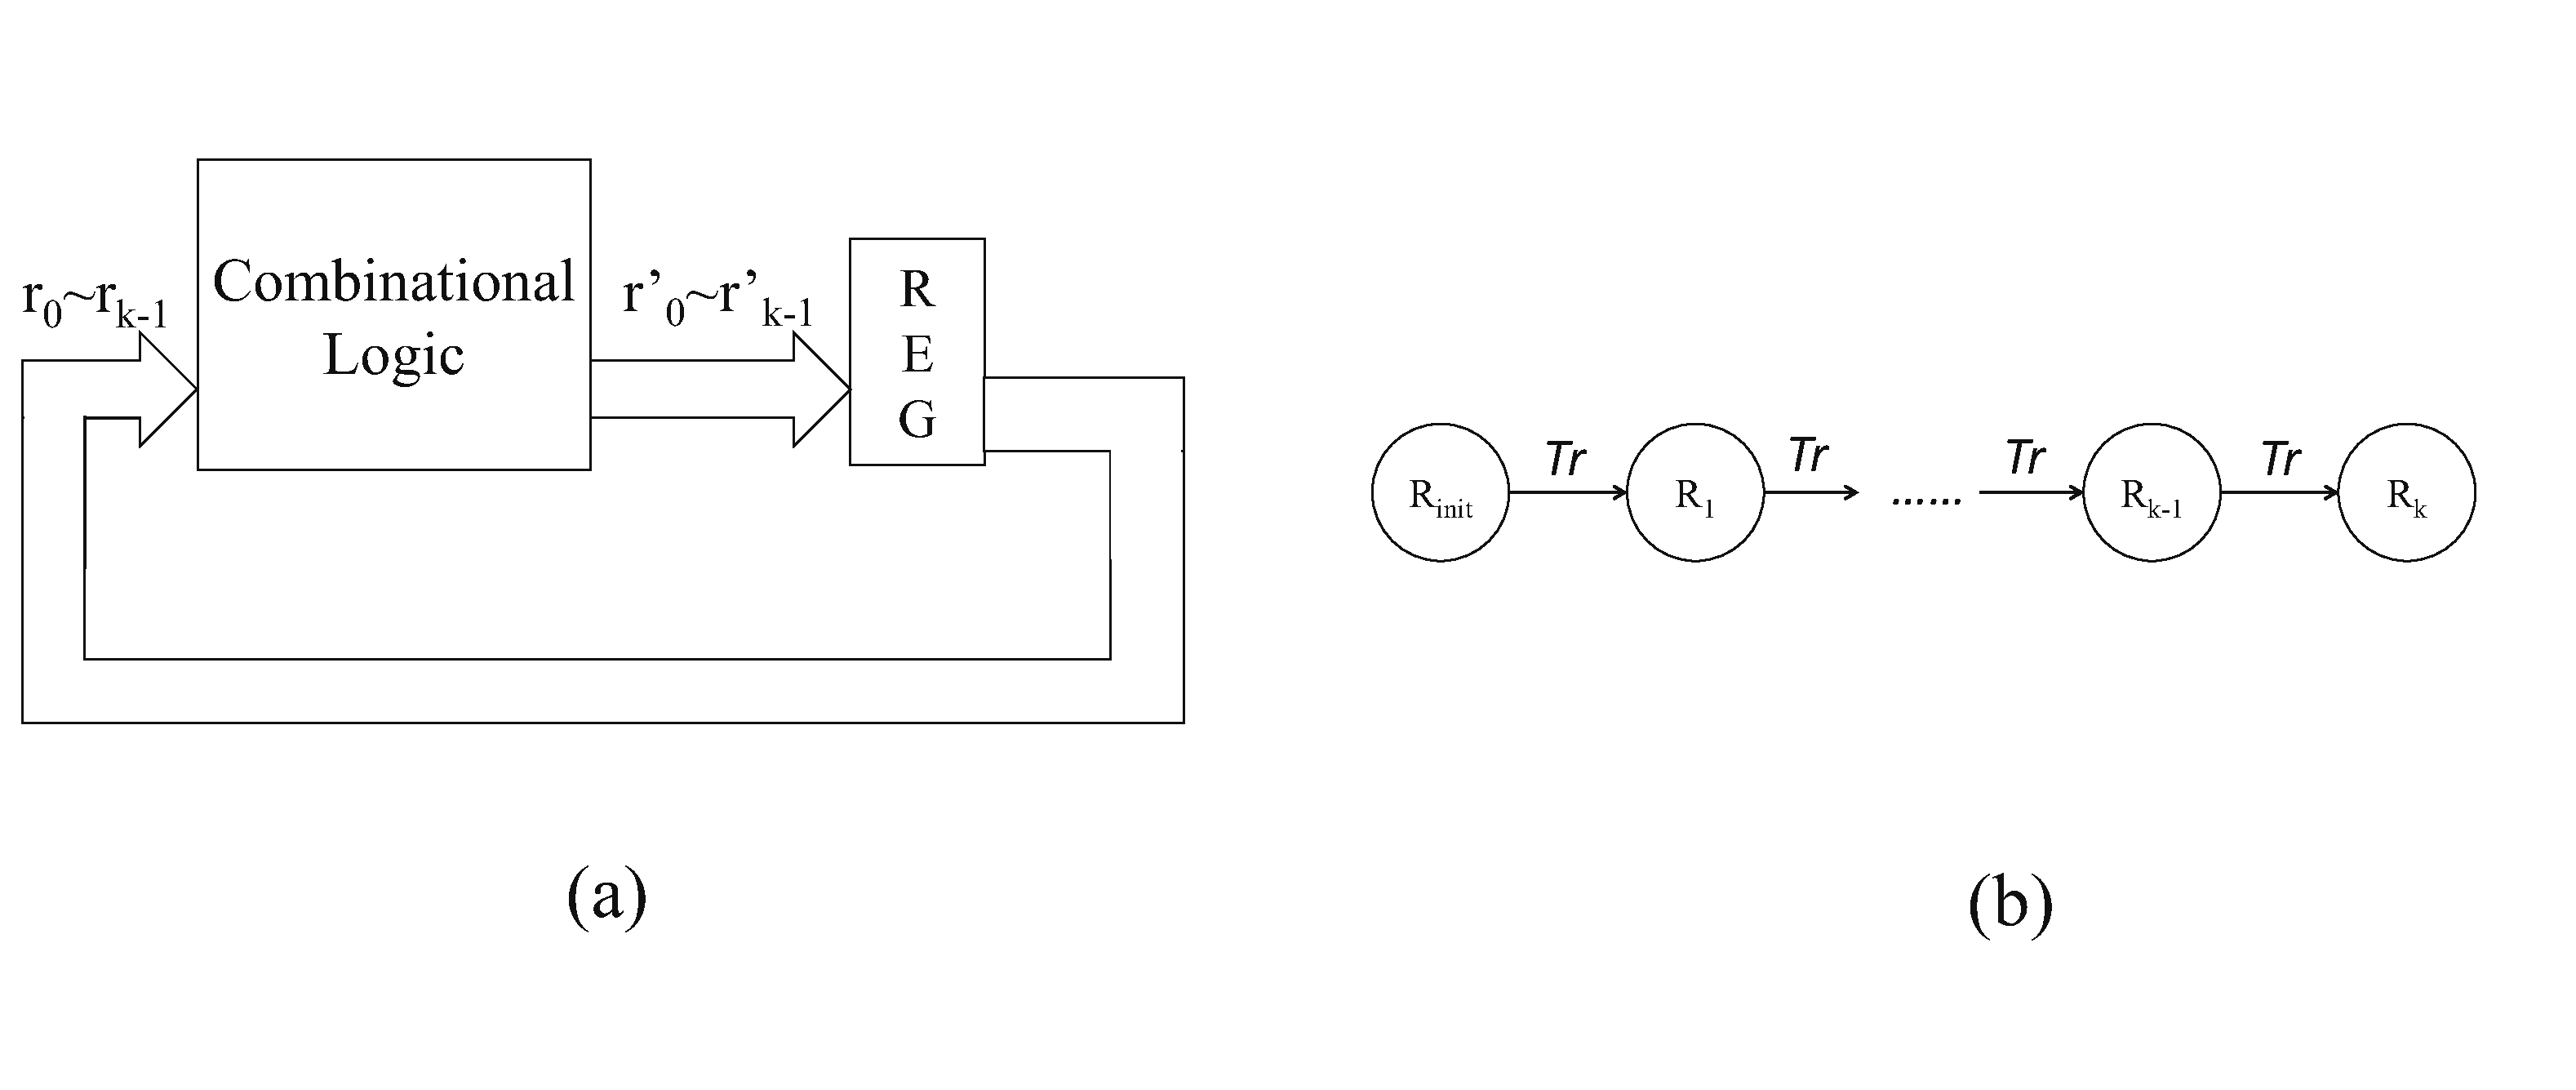
\includegraphics[width=7.5in]{./Moore.eps}
% % \vspace{-0.2in}
% \caption{A simple Moore FSM and its state transition graph}
% %\end{minipage}
% \label{fig:Moore}}
% \end{figure}

Fig.\ref{fig:seqmodel}(b) shows a typical Moore FSM without primary inputs, $R$ is the word-level state variable. Let word-level indeterminate 
$R_{init}$ denote the initial preloaded value of $R$, and $R_{i}$ denote the evaluation of $R$ after $i$ clock cycles
(transitions). Transition relation $Tr:R_{i-1}\to R_i$ can be modeled similar to
the image function in Algorithm \ref{alg:BFS}. Assume that after $k$ clock cycles, the machine should give a state output
$R_{k} = \mathcal F(R_{init})$. To verify this result, we can implicitly unroll this FSM and execute transition
function at word level for $k$ times, which is $R_{k} = Tr(R_{k-1}) = Tr(Tr(\cdots Tr(R_{init})\cdots)) = Tr^k(R_{init})$.

Sequential Galois field (GF) multiplier is a typical sequential arithmetic component widely used in cryptographic systems.
Since there is no primary input in the design, it can be regarded as Moore FSM (Fig.\ref{fig:RHmulti}(a))
where $R = \sum_{i=0}^{k-1} r_i \beta^{2^{i}}, ~A = \sum_{i=0}^{k-1} a_i
 \beta^{2^{i}}, ~B = \sum_{i=0}^{k-1} b_i \beta^{2^{i}}$. Notice that $\beta$ is the {\it normal element}
 which can be represented by a power of primitive element $\alpha:~\beta = \alpha^t$.
The states are encoded by evaluations of state variables, which can be implicitly verified 
by checking output-input function ($R = A\cdot B \pmod{P(\alpha)}$). 

% Additionally
% the inner structure of GF multiplier is XOR-rich such that we can test our approach on very large
% (>100 bits datapath) circuits.
% 
% Let us briefly describe the fundamentals behind the design of normal
% basis sequential GF multipliers, so as to put in perspective the type
% of designs that have been verified in this paper. Let $R =
% \sum_{i=0}^{k-1} r_i \beta^{2^{i}}, ~A = \sum_{i=0}^{k-1} a_i
% \beta^{2^{i}}, ~B = \sum_{i=0}^{k-1} b_i \beta^{2^{i}}$, then 
% \[
% R = A\cdot B = (\sum_{i=0}^{k-1} a_i \beta^{2^{i}}) (\sum_{j=0}^{k-1}
% b_j \beta^{2^{j}})  =
% \sum_{i=0}^{k-1}\sum_{j=0}^{k-1}a_ib_j\beta^{2^i}\beta^{2^j}\nonumber 
% \]
% 
% The expressions $\beta^{2^i}\beta^{2^j}$ are called cross-product
% terms and they can also be represented in normal basis: 
% \begin{displaymath}
% \beta^{2^i}\beta^{2^j} =
% \sum_{n=0}^{k-1}\lambda_{ij}^{(n)}\beta^{2^n}, \ \ \lambda_{ij}^{(n)}
% \in \Ftwo. 
% \end{displaymath}
% 
% From the above two equations, one can see that the expression for the
% $n^{th}$ digit of product $R = (r_0, \dots, r_n, \dots r_{k-1})$ is:
% \[
% r_n = \sum_{i=0}^{k-1}\sum_{j=0}^{k-1}\lambda_{ij}^{(n)}a_ib_j = A
% \cdot M_n \cdot B^T, ~~0 \leq n \leq k-1
% \]
% 
% where $M_n = (\lambda_{ij}^{(n)})$ is a binary $k \times k$ matrix over
% $\Ftwo$, and it is called the $\lambda$-matrix. 
%The collection of all
%$\{M_n\}$  $\lambda$-matrices is called the multiplication
%table. 
% Moreover, let $r_n = A \cdot M_n \cdot B^T$.
% Then $r_{n-1} = A \cdot M_{n-1} \cdot B^T = rotate(A) \cdot M_n
% \cdot rotate(B)^T$. This implies that $M_n$ is generated by right
% and down cyclic shifting $M_{n-1}$. Therefore, the hardware design
% of sequential GF multipliers is based on mappings of $A\cdot M_n
% \cdot B^T$ into AND-XOR gates and cyclic shift operations. 

% This paper verifies the implementation of two distinct 
% architectures of {\it sequential multipliers with parallel output
%   (SMPO)}, namely: i) the Agnew-SMPO  \cite{agnew1991implementation}
% by G. B. Agnew, which is a straight-forward implementation of the
% $\lambda$-matrix; and ii) the more recent, more complicated, yet very
% efficient RH-SMPO \cite{RHmulti}, by Reyhani-Masoleh and Hasan,
% depicted in Fig. \ref{fig:RHmulti}.  

In this proposal we use the verification of a sequential GF multiplier -- 
a 3-bit RH-SMPO invented by Reyhani-Masoleh and Hasan\cite{RHmulti} -- to illustrate our approach.
The normal element is given as $\beta = \alpha^3$, and primitive polynomial $P(\alpha) = \alpha^3+\alpha+1$.
The gate-level circuit is depicted in Fig.\ref{fig:RHmulti}(b).

\begin{figure}[hbt]
\centering{
%\begin{minipage}{12cm}
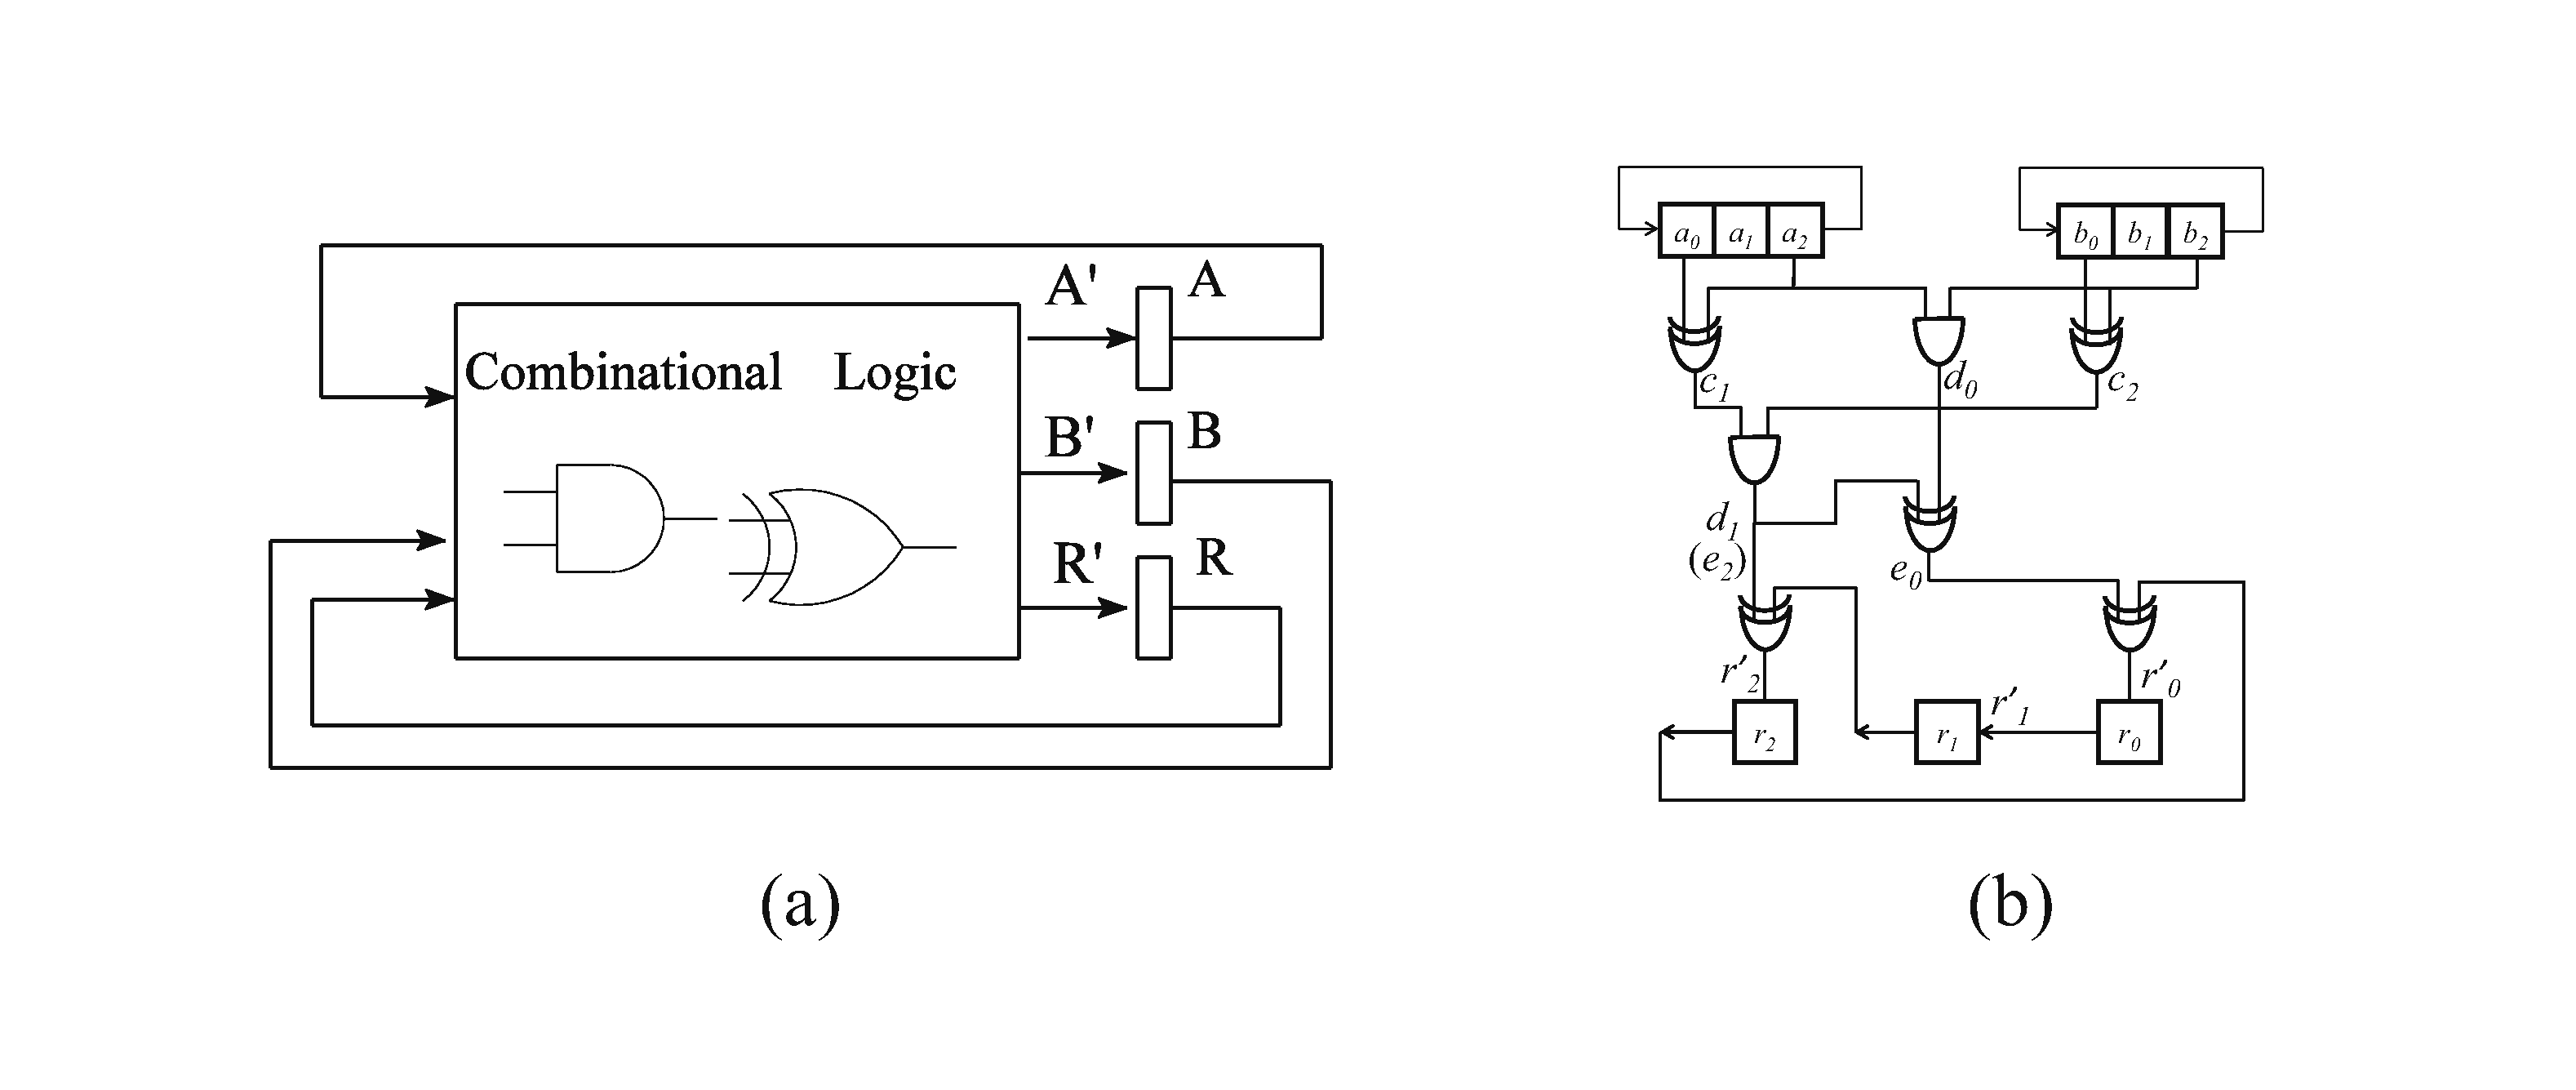
\includegraphics[width=7.5in]{./new_multi.eps}
% \vspace{-0.2in}
\caption{A 3-bit RH-SMPO and its Moore FSM model}
%\end{minipage}
\label{fig:RHmulti}}
\end{figure}

We follow  the typical sequential GF circuit model with word-level variables $A, B, R$
denoting {\it present states (PS)} and $A', B', R'$ denoting {\it next
  states (NS)} of the machine; where $A = \sum_{i=0}^{k-1} a_i \beta^{2^i}$
for the PS variables and $A' = \sum_{i=0}^{k-1} a_i'
\beta^{2^i}$ for NS variables, and so on.  Variables $R\ (R')$ correspond to those that 
store the result, and $A, B\ (A', B')$ store input operands. {\it E.g.,}
for a GF multiplier, $A_{init}, B_{init}$ (and $R_{init} =
0$) are the initial values (operands) loaded into the registers,  and
$R = \F(A_{init}, B_{init}) = A_{init} \times B_{init}$ is the final
result after $k$-cycles. Our approach aims to find this polynomial
representation for $R$.  

Each gate in the combinational logic is represented by a Boolean
polynomial. To 
this set of Boolean polynomials, we append the polynomials that define
the word-level to bit-level relations for PS and NS variables ($A =
\sum_{i=0}^{k-1} a_i \beta^{2^i}$). We denote this set of polynomials
as ideal $J = \langle 
f_1, \dots, f_s \rangle \subset \Fkk[x_1, \dots, x_d, R, R', A, A', B,
  B']$, where $x_1, \dots, x_d$ denote the bit-level (Boolean) variables
  of the circuit. The ideal of vanishing polynomials $J_0$ is also included, and
then the implicit FSM unrolling problem is setup for abstraction. 

The configurations of the flip-flops are the states of the
machine. {\it Since the set of states is a finite set of points, we
can consider it as the variety of an ideal related to the circuit
}. Moreover, since we are interested in
the {\it function encoded} by the state variables (over $k$-time
frames), we can {\it project this variety} on the word-level state
variables, starting from the initial state $A_{init}, B_{init}$.
Projection of varieties (geometry) corresponds to elimination ideals
(algebra), and can be analyzed via \Grobner bases. Therefore, we
employ a \Grobner basis computation with abstraction term order (ATO)\cite{timDAC}: we use a {\it lex term
  order} with {\it bit-level variables} 
$>$ {\it word-level NS outputs} $>$ {\it word-level PS inputs}. This
allows to eliminate all the bit-level variables 
%(corresponding to the combinational logic and the state variables),
%so as to 
and derives a representation only in terms of words. 
Consequently, $k$-successive \Grobner basis computations implicitly
unroll the machine, and provide word-level algebraic $k$-cycle
abstraction for $R'$ as $R' = \F(A_{init}, B_{init})$. 

Algorithm
\ref{alg:modified} describes our approach.  In the algorithm, $from_i$
and $to_i$ are polynomial ideals whose varieties are the valuations of
word-level variables $R, A, B$ and $R',A',B'$ in the $i$-th iteration;
and the notation ``$\setminus$'' signifies that the $NS$ in iteration
$(i)$ becomes the $PS$ in iteration $(i+1)$. Line 5 computes the Gr\"obner 
basis with the abstraction term order.  Line 6 computes the elimination 
ideal, eliminating the bit-level variables and representing the set of 
reachable states up to iteration $i$ in terms of the elimination ideal. 
These computations are analogous to those of image computations performed in FSM reachability. 
%The forward image
%$to^{i}$ is computed using \Grobner bases with ATO.

\vspace{-0.1in}
\IncMargin{1em}
\begin{algorithm}[hbt]
\SetAlgoNoLine
\LinesNumbered
 \KwIn{Circuit polynomial ideal $J$, vanishing ideal $J_0$, initial
   state ideal $R (=0), \mathcal{G}(A_{init}), \mathcal{H}(B_{init})$} 

  $from_0(R,A,B) = \langle R, \mathcal{G}(A_{init}), \mathcal{H}(B_{init})\rangle$\;
  $i = 0$\;
  \Repeat{$i == k$}
  {
  	$i \gets i + 1$\;
%	$to^i(R',A',B') \gets$  $GB( \langle J_{ckt}, J_0,
%    from^{i-1}(R,A,B)\rangle )$ with abstraction term order\;
	$G \gets$GB$( \langle J + J_0+ from_{i-1}(R,A,B) \rangle
    )$ with ATO\;
	$to_i(R',A',B')\gets G\cap \mathbb F_{2^k}[R',A',B',R,A,B]$\;
	$from_i \gets to_i(\{R,A,B\}\setminus \{R',A',B'\})$\;
  }
\Return{$from_k(R_{final})$}
\caption {Abstraction via implicit unrolling for Sequential GF circuit
  verification}
\label{alg:modified}
\end{algorithm}
\DecMargin{1em}
\vspace{-0.1in}
\begin{Example}
\label{ex:RHSMPO}

We demonstrate our approach to verify the 3-bit RH-SMPO circuit of
Fig.\ref{fig:RHmulti}. The normal element $\beta$ in
$\mathbb{F}_{2^3}$ is known to be $\beta = \alpha^3$, where $\alpha$
is the primitive element. The circuit can be described with an ideal by translating
AND and XOR gates accordingly. For the first iteration:
\begin{align*}
J = &d_0+b_2\cdot a_2,
c_1+a_0+a_2,
c_2+b_0+b_2,
d_1+c_1\cdot c_2,\\
&e_0+d_0+d_1,
e_2+d_1,
r_0'+r_2+e_0,
r_1'+r_0,
r_2'+r_1+e_2,\\
&A+a_0\alpha^3+a_1\alpha^6+a_2\alpha^{12},
B+b_0\alpha^3+b_1\alpha^6+b_2\alpha^{12},\\
&R+r_0\alpha^3+r_1\alpha^6+r_2\alpha^{12},
R'+r_0'\alpha^3+r_1'\alpha^6+r_2'\alpha^{12};
\end{align*}
The last 4 polynomials are translated from the definition of word-level variables.
This represents ideal ``$J$" from line 5 in Algorithm
\ref{alg:modified}. ``$J_0$" is the ideal of vanishing polynomials in all bit-level
variables (e.g. $a_0^2-a_0$) and word-level variables (e.g. $A^8-A$). ``$from_{i-1}$"
represents the set of current states for iteration $i$.
In the first iteration, $from_0 = \{R, A_{init}+a_0\alpha^3+a_1\alpha^6+a_2\alpha^{12},
B_{init}+b_0\alpha^3+b_1\alpha^6+b_2\alpha^{12}\}$.

After the GB computation is performed with ATO, as line 6 in Algorithm \ref{alg:modified},
we find a polynomial in variables $R', A_{init}, B_{init}$ in $to_1 : 
R'+(\alpha^2) A_{init}^4 B_{init}^4+(\alpha^2+\alpha) A_{init}^4 B_{init}^2+(\alpha^2+\alpha) A_{init}^4 B_{init}+(\alpha^2+\alpha) A_{init}^2 B_{init}^4+(\alpha^2+\alpha+1) A_{init}^2 B_{init}^2+(\alpha^2) A_{init}^2 B_{init}+(\alpha^2+\alpha) A_{init} B_{init}^4+(\alpha^2) A_{init} B_{init}^2
$.

Line 7 in Algorithm \ref{alg:modified} simply replaces NS output $R'$ with PS output
$R$ in this example; so in second iteration $from_1 = \{
R'+(\alpha^2) A_{init}^4 B_{init}^4+(\alpha^2+\alpha) A_{init}^4 B_{init}^2+(\alpha^2+\alpha) A_{init}^4 B_{init}+(\alpha^2+\alpha) A_{init}^2 B_{init}^4+(\alpha^2+\alpha+1) A_{init}^2 B_{init}^2+(\alpha^2) A_{init}^2 B_{init}+(\alpha^2+\alpha) A_{init} B_{init}^4+(\alpha^2) A_{init} B_{init}^2
, A_{init}+a_2\alpha^3+a_0\alpha^6+a_1\alpha^{12},
B_{init}+b_2\alpha^3+b_0\alpha^6+b_1\alpha^{12}\}$. 

% By continue executing the loop,
Finally, after 3 iterations we obtain: $to_3 = \{ \mathbf{R'+A_{init}B_{init},}
~A_{init}+a_0'\alpha^3+a_1'\alpha^6+a_2'\alpha^{12},
~B_{init}+b_0'\alpha^3+b_1'\alpha^6+b_2'\alpha^{12}\}$
as the image. The final result is $from_3(R_{final}) = R_{final}+A_{init}\cdot
B_{init}$, which verifies the multiplier. 
\end{Example}
Using our approach we successfully verified the function of an 100-bit RH-multiplier,
which implies its capability to handle the verification of large designs. The results
are published in \cite{myDATE}.
%\section{Overcoming the Limitations}
\subsection{Obviate GB computation}
Elimination ideal with ATO technique requires a GB computation, which is usually infeasible on large designs.
To obviate GB computation, we introduce a refinement on ATO as well as bit-word substitution method.

To overcome high computational complexity of GB calculation, \cite{pruss:dac14} proposed a
\underline{r}efinement of ATO (called RATO), and simplified the
\Grobner basis computation. They exploited Buchberger's product
criteria \cite{productc:1979}, which states that: {\it If the leading  
monomials of $f_i, f_j$ are relatively prime, then $Spoly(f_i, f_j)$
reduces to zero modulo the generating set, i.e. $Spoly(f_i, f_j)
\xrightarrow{F} _+ 0$.} This concept was exploited in RATO as follows: 

Perform a reverse topological sorting of the nodes in the
combinational logic, and define a {\it lex} term order by the
following relation $>_{r}$: {\it bit-level circuit variables ordered
  reverse topologically} $>$  {\it word-level output variables} $>$
{\it word-level input   variables}. Representing the polynomial ideal
$J$ in RATO has the effect that there exists {\it one and only one
  pair of polynomials} in $J$ that do not have relatively prime
leading terms (see  Section 5 in \cite{pruss:dac14} for details). All
other polynomial pairs will have leading terms that are 
relatively prime, so these polynomial pairs are not considered in
Buchberger's algorithm.  The authors of \cite{pruss:dac14} exploited
this concept and showed how the \Grobner basis of $(J + J_0)$ can be
computed by a {\it subset} of polynomials, which  improves the
scalability of their approach. Their approach, however, cannot
circumvent the \Grobner basis computation altogether. Consequently, 
their approach fails to derive a canonical polynomial abstraction when
the representation is dense, and contains monomials of high-degrees
(e.g. in case of buggy designs). 

Additionally, further improvements can be made to RATO:
With only RATO, the final remainder $h$ contains both bit-level variables and
word-level {\it state variables}. We desire
a polynomial in only word 
level variables without computing a
\Grobner basis. This can be achieved if we  represent the
bit-level state variables in terms of their word-level
variables. The basic idea of this improvement is: exploit the property of
polynomial squaring in $\Fkk$ to list $k$ polynomial equations,
use a Gaussian-elimination style technique to solve the system of equations.
Then we can substitute all bit-level variables in the remainder polynomial from RATO.
Details are described in our accepted DATE 2015 conference paper 
``{\it Formal Verification of Sequential Galois Field Arithmetic Circuits using Algebraic Geometry}".

\subsection{Complexity of multivariate division}
Using RATO and bit-word substitution, we can turn GB computation problem to a single multivariate division.
Although we gain success on verifying sequential GF multipliers, there are still problems when
doing implicit state enumerating on generic FSM. For example, when we tried to apply our approach
on ISCAS'89 benchmark s953 with 29 DFFs and 311 gates, RATO spent too much time on reducing
Spoly with ideal generators. By analyzing the process of polynomial reduction, we conjecture that
\begin{Conjecture}
Long chains of AND/OR gates will make polynomial reduction infeasible.
\end{Conjecture}

\begin{figure}[hbt]
\centering{
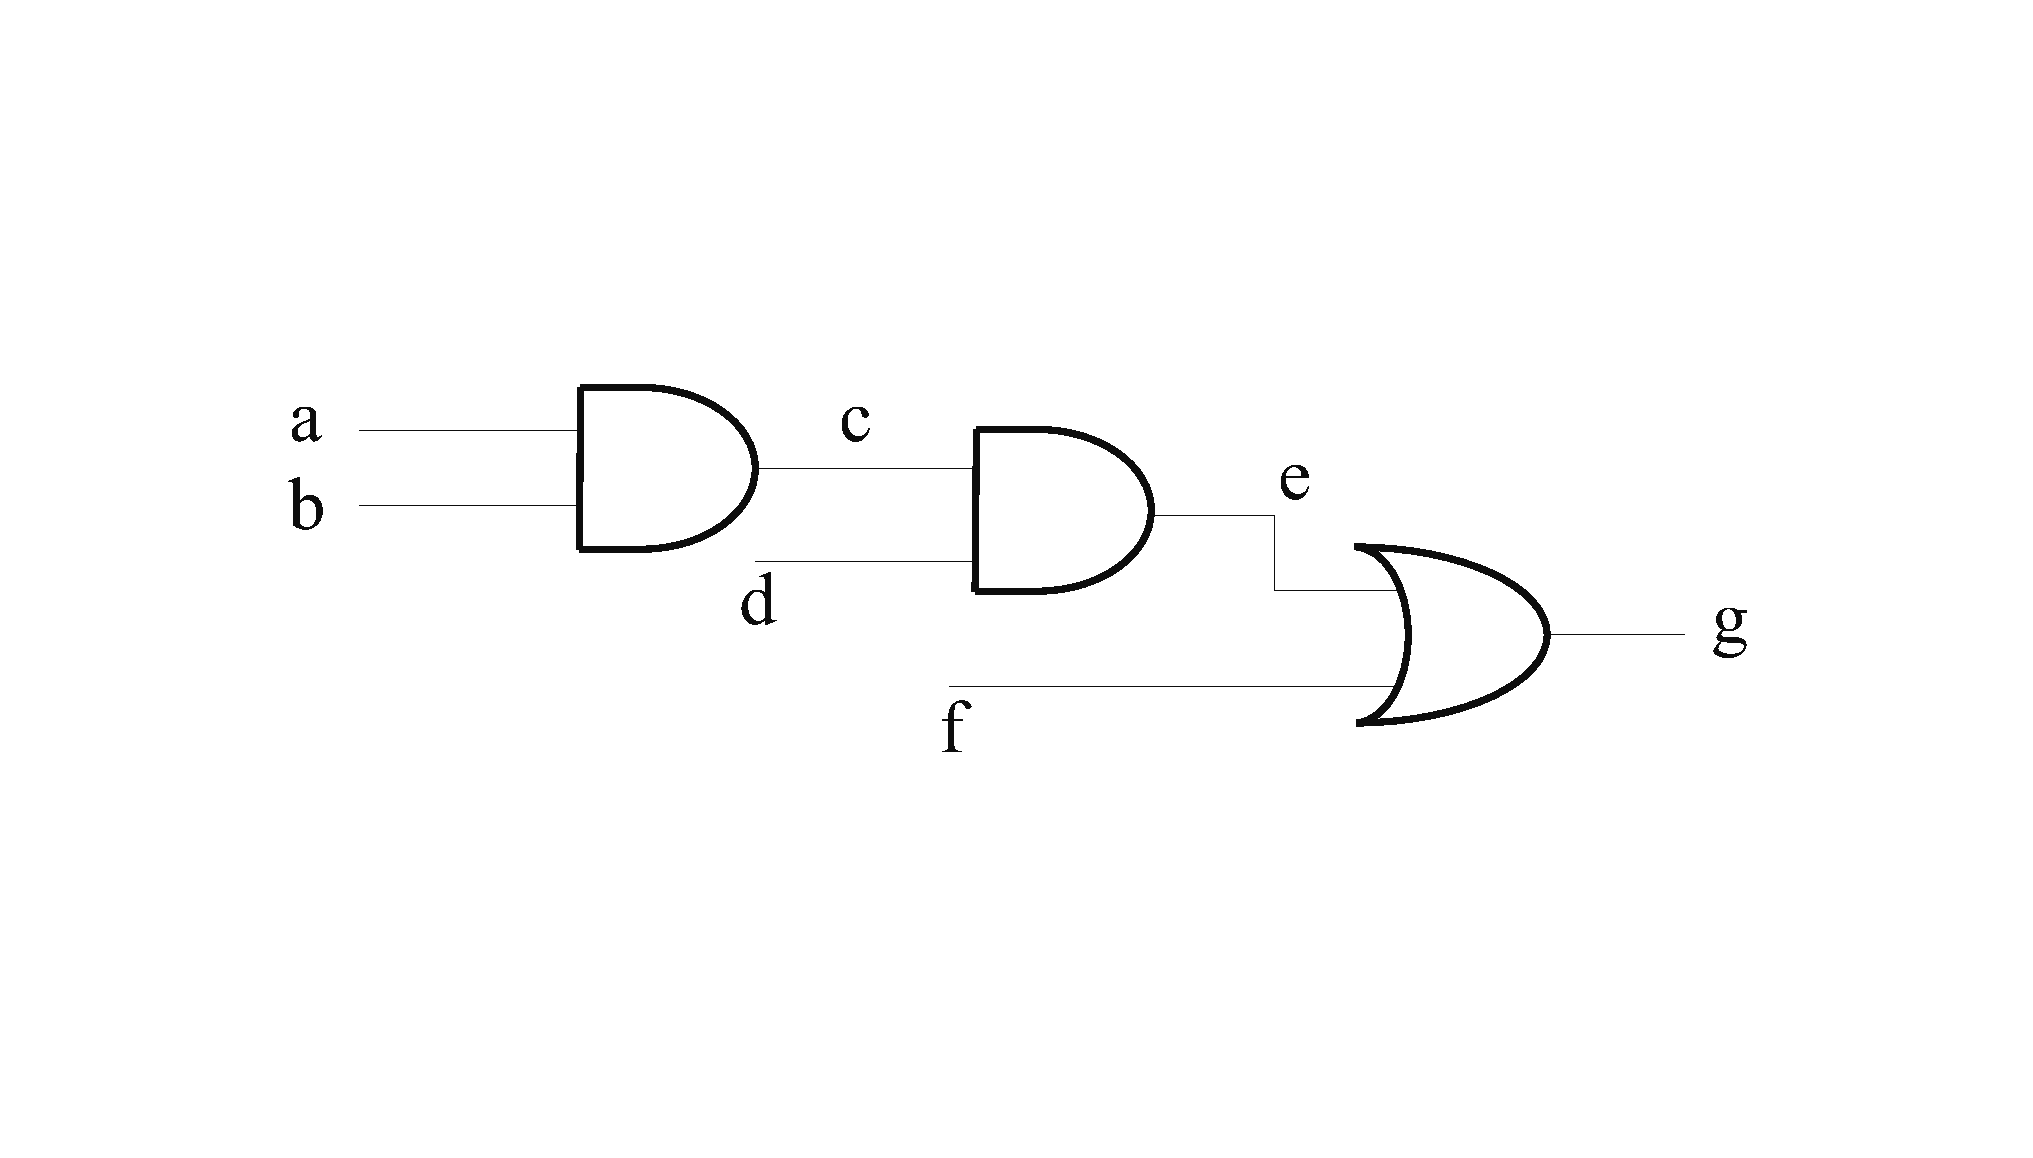
\includegraphics[scale=0.3]{./fig_chain.eps}
\caption{An example of AND-OR-gate chain}
\label{fig:chain}}
\end{figure}

\begin{Example}
Consider a chain (Fig.\ref{fig:chain}) of 3 gates: 2 AND gates and 1 OR gate. Write them in polynomials:
\begin{align*}
&h_1:g+ef+e+f\\
&h_2:e+cd\\
&h_3:c+ab
\end{align*}
Impose RATO: $g>e>c>\{a,b,d,f\}$. Reduce a simple polynomial $g$ with this set of polynomials:
$$g\xrightarrow{h_1}_{+} ef+e+f$$
$$g\xrightarrow{h_2}_{+} cdf+cd+f$$
$$g\xrightarrow{h_3}_{+} abdf+abd+f$$
We can conclude that:
\begin{itemize}
\item[-] When divided by polynomial from XOR gate, the length of remainder will increase by 1 term;
\item[-] When divided by polynomial from AND gate, the degree of remainder will increase by 1;
\item[-] When divided by polynomial from OR gate, the length and degree of remainder will increase by 1.
\end{itemize}
Since all gate polynomials have leading term with degree 1, a higher degree of remainder polynomial means
 more iterations of division (while a longer remainder does not always imply more divisions because
 there is still possibility to cancel multiple terms at one time). 
 Consider the querying time, a chain with AND/OR gates will blow up computational complexity of
reduction.

Sequential GF multiplier has only limited levels of gate chains (4 for RH-multiplier example). Although the size of 
datapath is large, actual complexity for reduction is relatively low.
\end{Example}

To lower down the complexity of reduction, we can introduce a matrix-based technique named as "F-4 style reduction" \cite{F4reduce}. 
It can speed up the procedure dividing a low-degree polynomial with term-sparse polynomial ideal. 

Another option is to cut back the cost of each univariate division. Horner's expansion diagram (HED)\cite{alizadeh2010modular}
is a graphical method to turn operations such as uniting like terms to lower complexity DAG manipulations.


\section{Using Algebraic Geometry to Assist in Abstraction refinement}
\subsection{Previous work}
Traditional methods to analyze sequential circuits require state variable encoding
as well as a complete/exact state enumeration with the initial state and transition function.
With the size of modern sequential circuits increasing, it is infeasible to apply conventional methods
any longer. Abstraction is a technique to minimize the state space representation by combining states with certain 
similarities. Sometimes it can effectively lower the number of states that require analysis by orders of magnitude,
without affecting the properties we need to verify.

At first, abstraction was done manually by designers. In 2000, E. Clarke \cite{clarke2000counterexample}
proposed an automated abstraction: first,
initial abstraction is set up by dividing variables to different clusters based on transition conditions;
then, an ordinary model checking is applied on this abstraction. If a counterexample is detected, 
it is further checked to be concrete or not. For a false abstract state or a spurious path 
, the initial abstraction is refined by further splitting the false abstract state. 
A heuristic algorithm keeps refining the abstraction until a real counterexample is found or the 
property is verified. This technique is based on binary decision diagrams (BDDs), which implies a
potential risk of memory explosion; meanwhile it still requires an initial abstraction to start with.

In 2004 L. Zhang and M. Hsiao \cite{zhang2005design} proposed another abstraction method based on CNF-SAT.
This paper uses simplest latch abstraction -- by removing "irrelevant" latches from the analysis. 
The key idea is to pick those ``irrelevant" latches (variables in $k$-bounded model checking, $k$-BMC) 
according to SAT/UNSAT analysis from the $k$-BMC. It improves the $k$-BMC procedure\cite{biere1999symbolic}: 
linear temporal logic (LTL) properties to check for can be translated to a (big) CNF formula and fed to a SAT solver. 
If SAT, a concrete counterexample is found. 
If UNSAT, the original method increases the bound $k$. In Zhang's paper, the clauses for UNSAT 
(UNSAT cores\footnote{UNSAT core is a subset of the original CNF clauses which are also unsatisfiable.})
are checked for variables that do not appear.
Thus an abstracted model is obtained and checked with the original property. If the abstracted model checking fails, 
then bound $k$ is increased. This method still has disadvantages: it is counterexample-independent,
which means it cannot utilize information from invariants.

In 2005, H. Jain et al.\cite{HimanshuDAC2005} improved the abstraction refinement technique of \cite{clarke2000counterexample},
where they use CNF-SAT to perform the refinement instead of using BDDs. The new approach is applied to verify RTL Verilog
and was known to be successful.

Abstraction usually means over-approximation, i.e. properties that are true on the abstracted machine
are also valid for the original states. Craig's interpolation is a sort of abstraction which may be either
over-approximation or under-approximation. In 2003, K. McMillan used Craig's interpolation to improve 
$k$-BMC \cite{mcmillan2003interpolation}. Initially a $k$-length path to failure state $F$ is picked and transformed to 
a CNF formula, then split at first transition into a prefix and a suffix. An interpolation $P$ is computed
between the prefix and suffix. $P$ over-approximates 1-step reachable states, and under-approximates states 
that cannot reach $F$ in $k$ steps. If no counterexample is exposed, the path is split again at the second
transition; in this way a precise abstraction can be found for all reachable states.

$k$-BMC with interpolation is a purely incremental model checking approach, and the interpolation procedure relies
on UNSAT core analysis. To overcome these weaknesses, a hybrid model checker named as IC3 is developed 
\cite{bradley2011sat} \cite{bradley2011incremental}. IC3 works incrementally to find out inductive subclauses
of negations of reached states, meanwhile it is monolithic when computing over-approximations to sets of reachable
states within $1,2,\dots,k$ steps. It is proved to be more efficient than interpolation based model checking
although using similar mechanisms.

\subsection{Exploiting UNSAT cores for abstraction refinement}
By exploring previous work, we learn that most state-of-art abstraction refinement techniques require 
information mining from UNSAT proofs of intermediate abstractions. 
Here we use an abstraction refinement algorithm from \cite{zhang2005design} to explain that how an UNSAT proof is
utilized in such techniques.

\begin{algorithm}[hbt]
\SetAlgoNoLine
	\KwIn{$M$ is the original machine, $p$ is the property to check, $k$ is the number of steps in $k$-BMC}
  $k = $ InitValue\;
  \eIf{$k$-BMC$(M,p,k)$ is \textbf{SAT}}
  {
	\Return{``Found error trace"}
  }
  {
	Extract UNSAT proof $\mathcal P$ of $k$-BMC\;
	$M' = $ \textit{ABSTRACT}$(M,\mathcal P)$\;
  }
  \eIf{MODEL-CHECK$(M',p)$ returns \textbf{PASS}}
  {
	\Return{``Passing property"}
  }
  {
	Increase bound $k$\;
	goto Line 2\;
  }
\caption {Abstraction refinement using $k$-BMC}\label{alg:absrefine}
\end{algorithm}
\begin{figure}[hbt]
\centering{
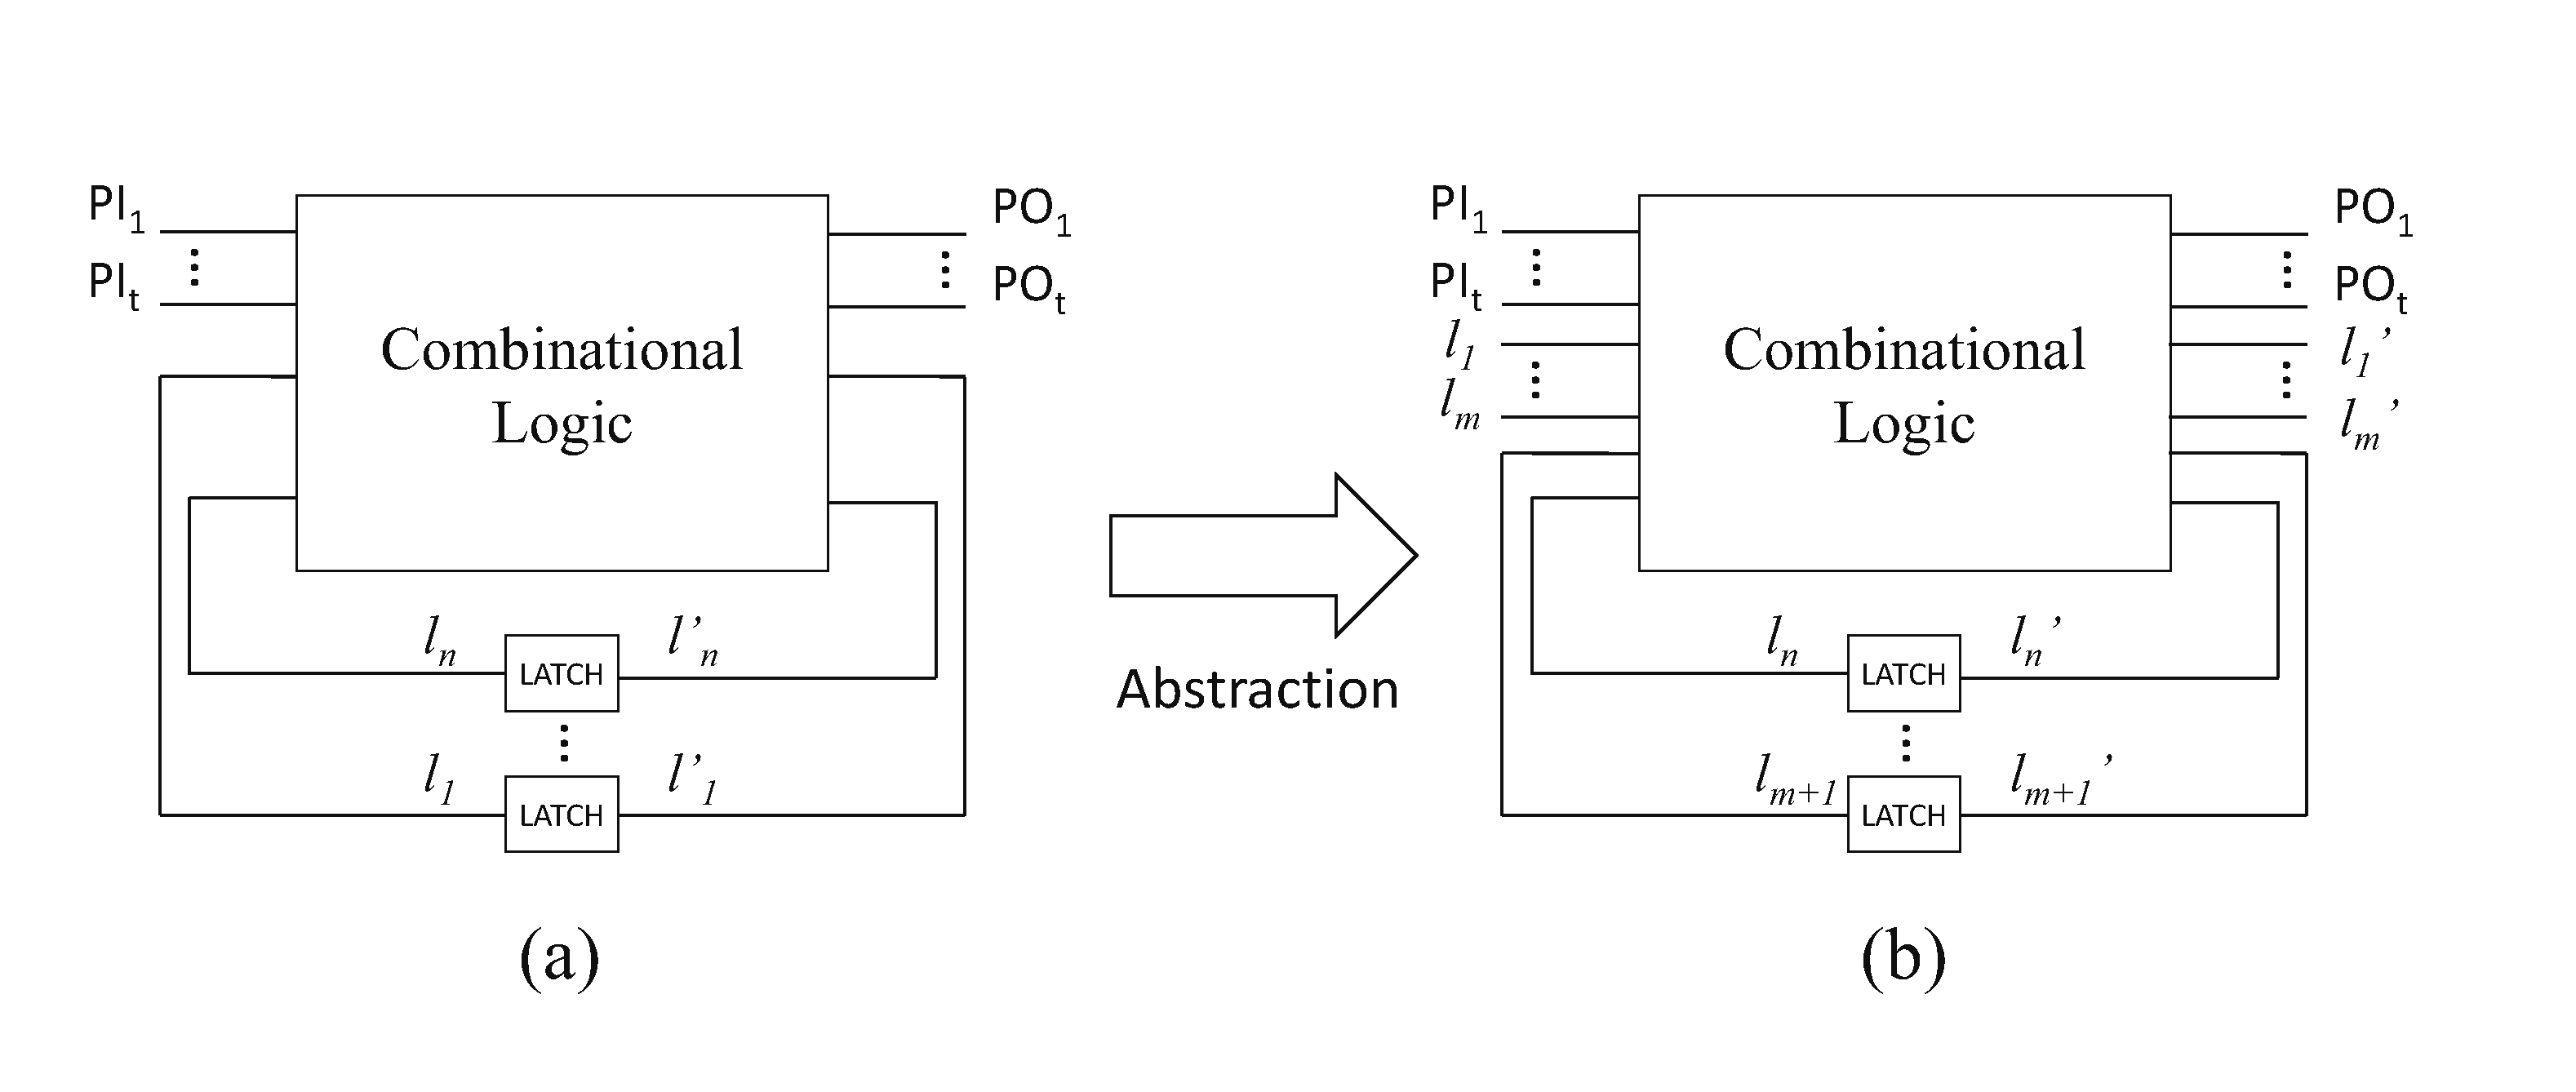
\includegraphics[width=5.5in]{./refine.eps}
\caption{Abstraction by reducing latches}
\label{fig:refine}}
\end{figure}
Assume that we are given a sequential circuit with $n$ latches as shown in Fig.\ref{fig:refine}(a). 
This circuit can be modeled as a Mealy machine $M$ and the states $s$ can be explicitly encoded by bit-level latch variables 
$l_1,\dots,l_n$. Algorithm \ref{alg:absrefine} describes an approach to check if machine $M$ violates property $p$.
This algorithm relies on $k$-BMC technique, which works on the basis of CNF-SAT solving.
The $k$-BMC represents the initial states $I$, the transition relation $T$ and property $p$ as CNF formulas.

The first ``if-else" branch in Algorithm \ref{alg:absrefine} can be
explained as: we check if the conjunction of formulas 
$$I(s_0)\land \bigwedge_{i=0}^{k-1}T(s_i,s_{i+1}) \land \neg p$$
is $SAT$ or not, where $s_i$ denotes the set of reached states in $i$-th time-frame. If the result is
$SAT$, then a counterexample is found that violates property $p$. If the result is $UNSAT$, we cannot
assert that $p$ is satisfied for the original machine $M$ because we only unrolled $M$ for a given specific number of time-frames
without any fixpoint detected.
In this algorithm, we analyze the UNSAT core composed by a set of clauses whose conjunction is $UNSAT$.
If there are some latch variables not included in this UNSAT core (denoted by $L_{abs}$), then we can assert that the evaluations of 
these variables will not affect the unsatisfiability of original formula. Therefore, we can ignore them in the abstracted model.
In practice, we turn these latches into primary inputs/outputs as shown in Fig.\ref{fig:refine}(b) ($L_{abs} = \{l_1,\dots,l_m\}$).


The second ``if-else" branch means: if we do an ordinary model checking on the abstracted machine $M'$ and find no
error trace, we can assert that property $p$ also holds on the original machine $M$. The reason of this assertion is that
the abstracted states represented using abstracted latches cover the original states, which means $M'$ is an over-approximation
of $M$, such that $(M'\implies p) \implies (M\implies p)$. If we find a violation on abstracted machine, then this
abstracted model is not a suitable model to check $p$, so we have to increase the bound $k$ to find a finer abstraction.

It is clear that UNSAT cores play an important role in abstraction refinement approaches. In \cite{zhang2005design}
the UNSAT core is extracted using a conventional CNF-SAT solver, which will encounter the ``bit-blasting" problem
when the size of datapath (number of latches in Fig.\ref{fig:refine}) is very large. \textbf{Here we propose a totally new 
method based on Gr\"obner basis computation to extract UNSAT cores, and we believe it may become an efficient 
method according to the following observation based on our experience:}

% {\it Gr\"obner basis is more suitable for UNSAT problems because of following theorem:}
{\it While computing GB over finite fields is exponential in the number of variables, GB  computation 
is observed to be more efficient for UNSAT problems.} 
The reason is discussed as follows:
\begin{Theorem}
{\bf Weak Nullstellensatz:} Given ideal $J\subset \mathbb F[x_1,\dots,x_n]$, its variety over algebraic closure
of field $\mathbb F$ is empty if and only if its reduced Gr\"obner basis contains only one generator ``1".
$${\bf V}_{\overline{\mathbb F}}(J) = \emptyset \Longleftrightarrow reducedGB(J) = \{1\}$$
\end{Theorem}
It is well known that using Buchberger's algorithm and its variations to compute a GB has a very high
time complexity and is usually not practicable. One reason is that the size of GB may explode even if the term
ordering is carefully chosen. However if the reduced GB is 1, which means every term in the original polynomials
will be canceled, the degree of remainders when computing GB with Buchberger's algorithm will be limited. 
Thus the number of polynomials in non-reduced GB is much smaller than usual.
Instead of applying polynomial calculus to SAT solving, it may be more efficient to try it for UNSAT
problems.

\subsection{A demonstration of our conjecture}
One  important research topic about UNSAT problems is to identify UNSAT cores efficiently.
An UNSAT core in a CNF formula denotes a subset of clauses which is still unsatisfiable. Here
we re-define this concept in algebraic geometry:
\begin{Definition}
Assume a set of polynomials $F$ and its subset $F_s\subset F$. If ${\bf V}(\langle F\rangle) = {\bf V}
(\langle F_s\rangle) = \emptyset$, we call $F_s$ an {\bf UNSAT core} of $F$. Additionally, if
$F_s$ contains no other UNSAT core, we call it a {\bf minimal} UNSAT core.
\end{Definition}

We  conjecture that based on observation of Buchberger's algorithm's execution, an UNSAT core can be identified.
\begin{Conjecture}
Buchberger's algorithm picks pairs of polynomials from a given set, computes their S-poly, then reduces this S-poly
with the given set of polynomials. If the remainder is non-zero,
it is added to the set of polynomials.
By tracking S-poly computations and multivariate divisions that lead to remainder 
1, we can obtain an UNSAT core. Moreover, we can identify a minimal UNSAT core with one-time
 execution of Buchberger's algorithm.
\end{Conjecture}
\begin{Example}
A SAT problem is described with 8 CNF clauses:

\begin{minipage}[h]{0.3\textwidth}
\begin{align*}
&c_1: \bar{a}\lor\bar{b}\\
&c_2: a\lor\bar{b}\\
&c_3: \bar{a}\lor b\\
&c_4: a\lor b
\end{align*}
\end{minipage}
\begin{minipage}[h]{0.7\textwidth}
\begin{align*}
&c_5: x\lor y\\
&c_6: y\lor z\\
&c_7: b\lor \neg y\\
&c_8: a\lor x\lor \neg z
\end{align*}
\end{minipage}

% \begin{align*}
% &\bar{a}\lor\bar{b}\\
% &a\lor\bar{b}\\
% &\bar{a}\lor b\\
% &a\lor b\\
% &x\lor y\\
% &y\lor z\\
% &b\lor \neg y\\
% &a\lor x\lor \neg z
% \end{align*}
Using Boolean to polynomial mappings given in Table \ref{tab:booltof4}, we can transform them to a set of
polynomials $F$ over ring $\mathbb F_2[a,b,x,y,z]$:

\begin{minipage}[h]{0.4\textwidth}
\begin{align*}
&f_1:ab\\
&f_2:ab+a\\
&f_3:ab+b\\
&f_4:ab+a+b+1
\end{align*}
\end{minipage}
\begin{minipage}[h]{0.6\textwidth}
\begin{align*}
&f_5:xy+y+x+1\\
&f_6:yz+y+z+1\\
&f_7:by+y\\
&f_8:axz+az+xz+z
\end{align*}
\end{minipage}
% \begin{align*}
% &f_1:ab\\
% &f_2:ab+a\\
% &f_3:ab+b\\
% &f_4:ab+a+b+1\\
% &f_5:xy+y+x+1\\
% &f_6:yz+y+z+1\\
% &f_7:by+y\\
% &f_8:axz+az+xz+z
% \end{align*}
We compute its GB using Buchberger's algorithm with lexicographic term ordering $a>b>x>y>z$.
Since this problem is UNSAT, we will stop when ``1" is added to GB.
\begin{enumerate}
\item First we compute $Spoly(f_1,f_2)\xrightarrow{F}_{+} r_1$, remainder $r_1$ equals to $a$;
\item Update $F=F\cup r_1$;
\item Next we compute $Spoly(f_1,f_3)\xrightarrow{F}_{+} r_2$, remainder $r_2$ equals to $b$;
\item Update $F=F\cup r_2$;
\item We can use a directed acyclic graph (DAG) to represent the process to get $r_1,r_2$, as Fig.\ref{fig:UNSAT}(a) shows;
\item Then we compute $Spoly(f_1,f_4) = s_3= a+b+1$, obviously $a+b+1$ can be reduced (multivariate divided) by
$r_1$ , the intermediate remainder $r_3 = b+1$. It can be immediately divided by $r_2$, and the remainder is ``1", we
terminate the Buchberger's algorithm;
\item We draw a DAG depicting the process through which we obtain remainder ``1" as shown in Fig.\ref{fig:UNSAT}(b). 
From leaf ``1" we backtrace the graph to roots $f_1,f_2,f_3,f_4$. They constitute an UNSAT core for this problem
as these polynomials are the ``causes" of unsatisfiability of original set of clauses.
\end{enumerate}
\end{Example}
\begin{figure}[hbt]
\centering{
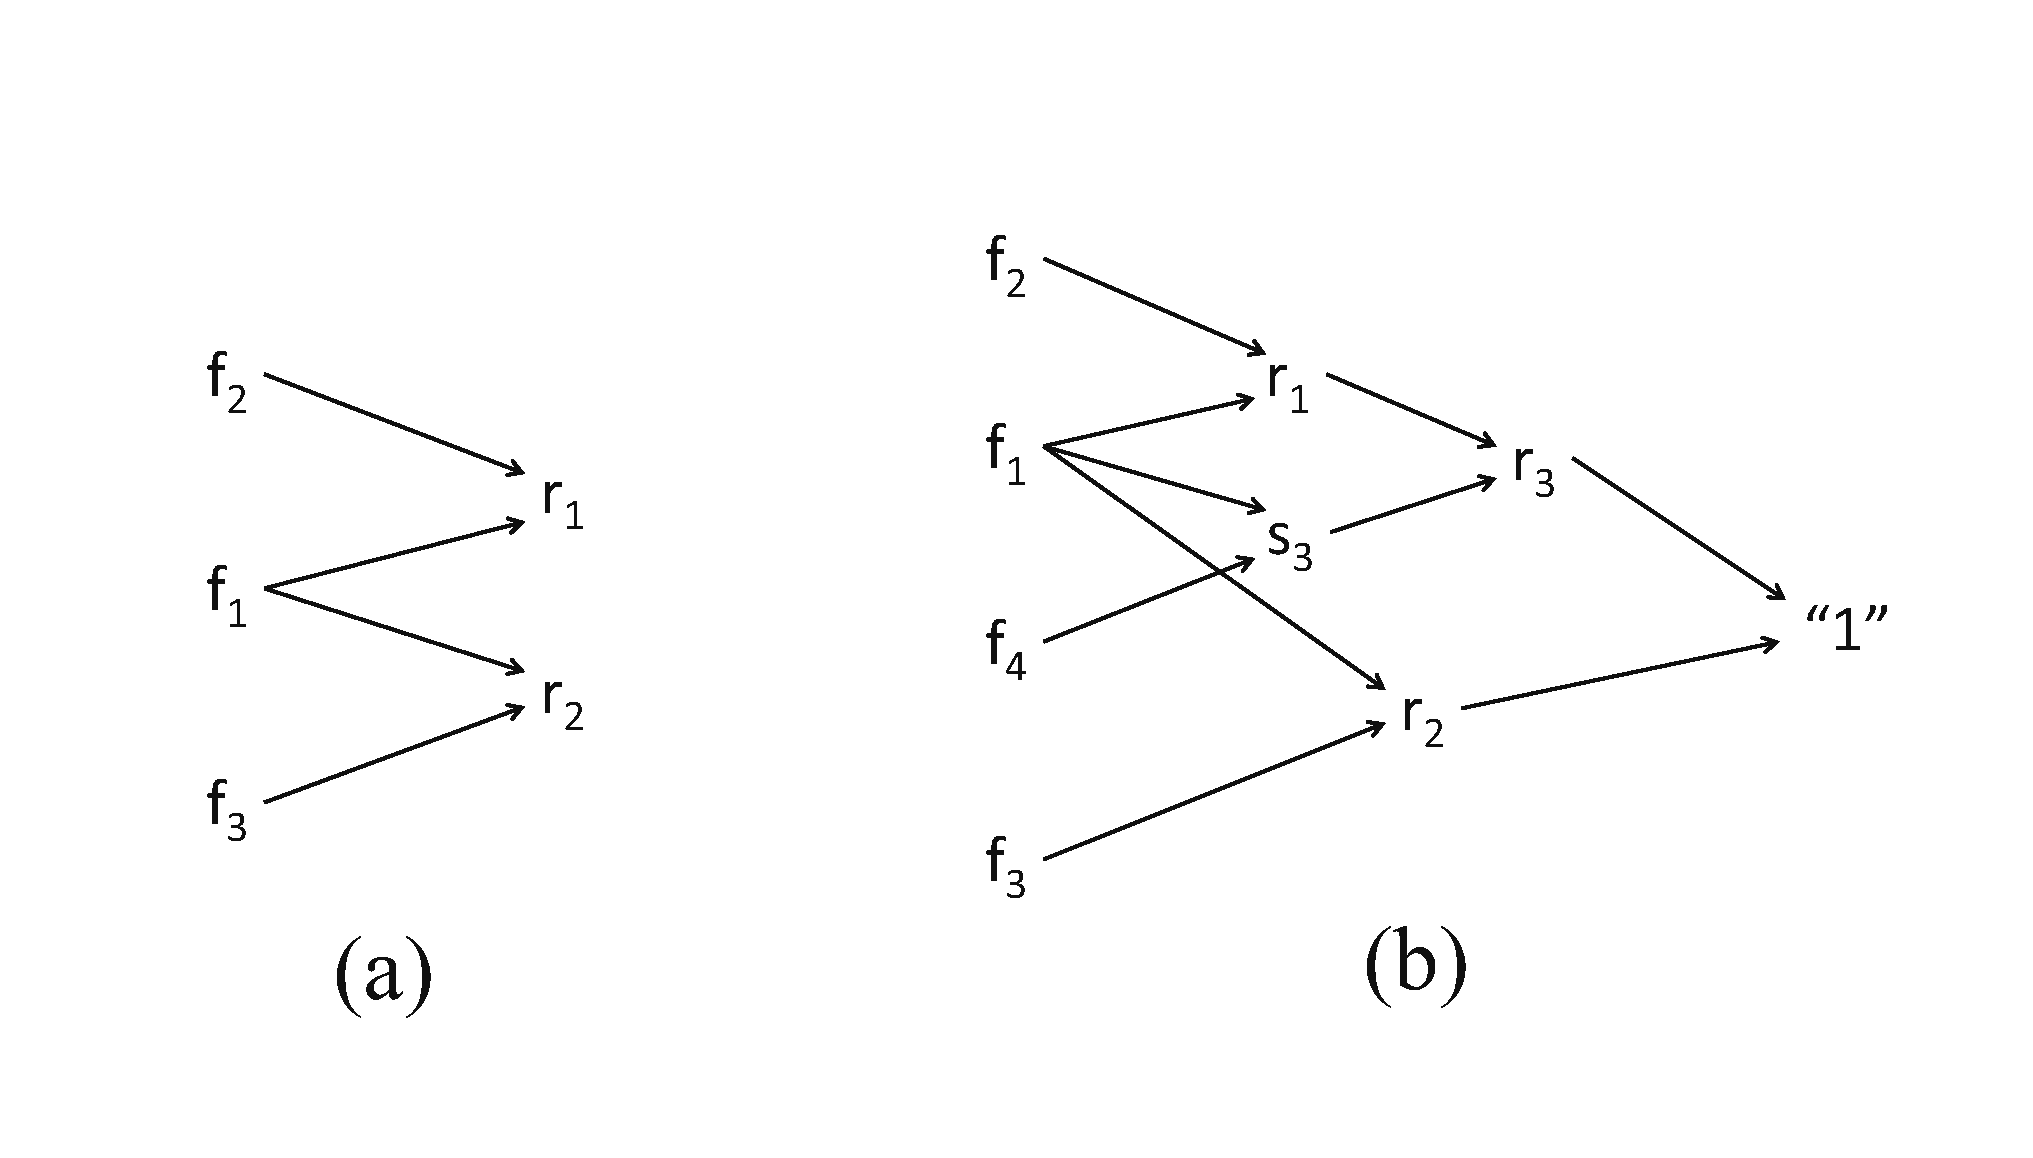
\includegraphics[width=4.5in]{./UNSAT.eps}
\caption{DAG representing Spoly computations and multivariate divisions}
\label{fig:UNSAT}}
\end{figure}
% We conclude our approach as follows: i) Keep track of all $Spoly(f_i,
% f_j)\xrightarrow{f_1, \dots, f_s}_+ r$; ii) mark $f_i, f_j$ if $r\neq
% 0$; iii) Mark those $f_l$'s that have leading terms that cancel
% monomial terms in $Spoly(f_i, f_j)$; iv) Build a DAG recording all reductions including Spoly computations
% and multivariate divisions; v) Once $1\in J$ is
% detected, traverse the graph to identify all the marked polynomials that were
% used in obtaining this unit element. These polynomials constitute the
% core.

We conclude our approach as a conjecture algorithm (Algorithm \ref{alg:UNSAT}). 

\begin{algorithm}[hbt]
\SetAlgoNoLine
	\KwIn{A set of polynomials $F = \{f_1,f_2,\dots,f_s\}$}
	\KwOut{An UNSAT core $\{f_{m_1},f_{m_2},\dots,f_{m_t}\}$}
\Repeat{$r_l == 1$}
{
	Pick a pair $f_i,f_j\in F$ that has never been computed S-poly\;
	\If{$Spoly(f_i,f_j)\xrightarrow{F}_+ r_l \neq 0$}
	{
		$F = F\cup r_l$\;
		Create a DAG $G_l$ with $f_i,f_j$ as roots, $r_l$ as leaf, recording the S-poly, all intermediate remainders and $f_k\in F$ that cancel monomial terms in the S-poly\;
	}
}
Backward traverse the DAG for remainder ``1", replace $r_l$ with corresponding DAG $G_l$\;
\Return{All roots}
\caption {Extract UNSAT core using a variation of Buchberger's algorithm}\label{alg:UNSAT}
\end{algorithm}

\subsection{Research objective}
i) To prove that the algorithm is concrete and complete: it can always abstract an UNSAT core;

ii) To design an algorithm to find a minimal UNSAT core;

iii) Run the algorithm at word level, to find UNSAT proofs for word-level variables in $\Fkk$, which 
can help word-level abstraction refinement procedure.

% If we start with other term orderings, we may get a larger UNSAT core. By dynamically adjusting
% term ordering and re-calculate GB, we can get new UNSAT core with smaller size, until
% we find minimal UNSAT core or expire runtime limit.
\section{Proposed Objectives}
\begin{itemize}
\item[-] Explore an implementation of algebraic geometry based reachability analysis for sequential circuits verification;
\item[-] Currently our approach is implemented within the {\sc Singular} tool, which is not efficient enough to execute our
proposed algorithms, because its data-structures are not efficient for circuit verification problems. We plan to design a standalone CAD tool implemented in C++, which specifically aims to solve word-level sequential
verification problems. We will borrow techniques from \cite{timDAC}, \cite{jinpeng} and \cite{f4reduce}, and tailor them to sequential circuit analysis, to lower the computational
complexity;
\item[-] Fine-tune the tool for sequential Galois field arithmetic circuits verification, because arithmetic circuit
verification greatly benefits from the abstraction of word-level operands in the datapath;
\item[-] Explore a new abstraction-refinement paradigm, based on information from UNSAT cores, which is also 
attained using a Gr\"obner basis approach.
\end{itemize}

\section{Proposed Timetable}
\begin{itemize}
\item[-] Current status: Experiments have been performed to run implicit state enumeration on sequential circuits benchmarks
such as ISCAS'89 circuits. Current problem is the algorithm spends too much time on multivariate division procedure;
\item[-] Spring 2015: Implement the tool which can efficiently do multivariate division and test the performance of 
our tool based on T. Pruss et al's \cite{timDAC} approach;
\item[-] Summer 2015: Integrate the refined multivariate division routine into our verification tool, test its
performance on circuits with various sizes;
\item[-] Fall 2015: Evaluate data and write the dissertation.
\end{itemize}
%%%%%%%%%%%%%%%%%%%% The bibliography %%%%%%%%%%%%%%%%%%%%%%%%%%%%
\bibliographystyle{ieee}
\bibliography{xiaojun,logic,oldlogic,normalbasis}

\end{document}

%%%%%%%%%%%%%%%%%%%%%%%%%%%  End of IEEEsample.tex  %%%%%%%%%%%%%%%%%%%%%%%%%%%
